% !TeX program = pdflatex
\documentclass[11pt]{amsart}

\usepackage[dvipsnames]{xcolor}
\usepackage{enumitem}
\usepackage{amssymb,graphicx,mathtools,microtype}
\usepackage{nicefrac}
\usepackage{tikz}
\usetikzlibrary{arrows.meta}
\usepackage[margin=1in]{geometry}
\geometry{letterpaper}
\usepackage{etoolbox}
\usepackage[square,longnamesfirst]{natbib}
\renewcommand{\bibfont}{\small}
\AtBeginEnvironment{thebibliography}{\raggedbottom}

\theoremstyle{plain}
\newtheorem{theorem}{Theorem}[section]
\newtheorem{proposition}[theorem]{Proposition}
\newtheorem{lemma}[theorem]{Lemma}
\theoremstyle{definition}
\newtheorem{problem}{Problem}[section]
\newtheorem{remark}[theorem]{Remark}

\newcommand{\Z}{\mathbb Z}
\newcommand{\R}{\mathbb R}
\renewcommand{\P}{\mathbb P}
\newcommand{\E}{\mathbb E}
\newcommand{\Var}{\operatorname{Var}}
\newcommand{\drift}{\varepsilon}
\newcommand{\gauge}{\Psi}
\newcommand{\ind}{\mathbf 1}
\newcommand{\dd}{\,\mathrm d}
\newcommand{\defn}[1]{\textbf{#1}}
\newcommand{\nf}{\nicefrac}
\newcommand{\Rin}{R_{\mathrm{in}}}
\newcommand{\Rout}{R_{\mathrm{out}}}
\newcommand{\Rmom}{R_{\mathrm{mom}}}
\setcounter{secnumdepth}{2}
\numberwithin{equation}{section}

\makeatletter
\patchcmd{\@settitle}{\uppercasenonmath\@title}{\Large}{}{}
\patchcmd{\@setauthors}{\MakeUppercase}{\large}{}{}
\makeatother

\usepackage[citecolor=PineGreen,colorlinks=true,
linkcolor=RoyalBlue,urlcolor=BrickRed]{hyperref}
\hypersetup{pdftitle={Limit shapes of centrally excited random walks},
pdfauthor={Ahmed Bou-Rabee and Yuval Peres}}

\title[Limit shapes of centrally excited walks]{Limit shapes of centrally
excited random walks}
\author{Ahmed Bou-Rabee}
\address{Department of Mathematics, University of Pennsylvania,
Philadelphia, PA 19104, USA}
\email{ahmedmb@sas.upenn.edu}
\author{Yuval Peres}
\address{Beijing Institute of Mathematical Sciences and Applications,
Beijing 101408, China}
\email{yperes@bimsa.cn}
\subjclass[2020]{Primary 60K35; Secondary 60G50, 60G42, 31C20}
\keywords{Excited random walk, self-interacting walks, limit shapes,
norms, local times, martingale central limit theorem, law of the iterated
logarithm}
\date{}

\begin{document}

\begin{abstract}
A centrally excited random walk on $\Z^d$ moves like simple random walk, except that its first step from each site has a drift of fixed size toward the origin. Kozma (2007) conjectured that after $n$~steps the visited set approximates a ball of radius of order~$n^{\nf{1}{(d+1)}}$. We prove this in every dimension $d\geq2$ and show that the rescaled numbers of visits converge uniformly to a cone, which is the potential generated by the drift on a ball. The same argument shows that a drift opposite to a subgradient of a norm produces the ball of that norm. In the plane, the outer and inner radii of the visited set differ by at most $ n^{1/6}$ times a power of~$\log n$, and the exponent~$1/6$ cannot be lowered.
\end{abstract}

\maketitle

\begin{figure}[!b]
\centering
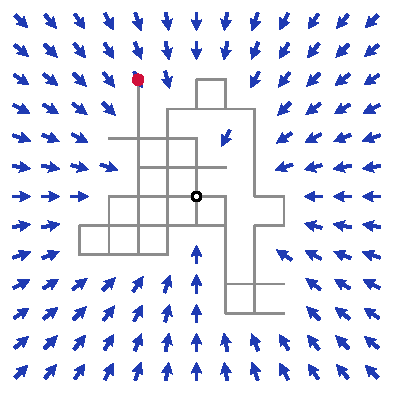
\includegraphics[width=0.5\textwidth]{Figures/first_departure_norms.pdf}
\caption{The walk after $120$~steps, for $d=2$ and $\drift=0.4$: its path (gray), the origin (open circle) and its position (red dot). At each site~$x\neq0$ that it has not yet left, an arrow shows the mean $-\drift x/|x|$ of its first step from~$x$.}
\label{fig:mechanism}
\end{figure}

\section{Introduction}\label{sec:introduction}

Let $d\geq2$ and $0<\drift<1/d$. A \defn{centrally excited random walk} $X_0=0,X_1,X_2,\ldots$ on~$\Z^d$ moves like simple random walk, except that on its first departure from each site~$x\neq0$ it moves to $x\pm e_i$ with probability~$1/(2d)\mp\drift x_i/(2|x|)$ for $1\leq i\leq d$, where $e_1,\ldots,e_d$ is the standard basis of~$\R^d$. Given the path up to that departure, this step has mean~$-\drift x/|x|$, a drift of size~$\drift$ toward the origin (Figure~\ref{fig:mechanism}).

At an Oberwolfach problem session, \citet{Oberwolfach2007} conjectured that the visited set approximates a ball of radius of order~$n^{\nf{1}{(d+1)}}$. We prove this for every $d\geq2$, identify the radius and the uniform limit of the local times, and bound their fluctuations. In the plane the radii fluctuate on the scale~$n^{\nf16}$ up to logarithmic factors; in higher dimensions they are bounded by powers of~$\log n$. More generally, a first-departure drift opposite to a subgradient of a norm produces the ball of that norm.

\subsection{The limit shape}\label{sec:shape}

For an integer~$n\geq0$ let
\begin{equation*}
\ell_n(x)\coloneqq\sum_{j=0}^{n-1}\ind_{\{X_j=x\}}
\qquad\text{and}\qquad
A_n\coloneqq\{x:\ell_n(x)>0\}\, .
\end{equation*}
The \defn{local time}~$\ell_n(x)$ is the number of departures from~$x$ before time~$n$, and $A_n$ is the \defn{range}; the set of sites visited by time~$n$ is~$A_{n+1}$. Write $B(y,\rho)$ for the open Euclidean ball of radius~$\rho$ about~$y$ and $\omega_d$ for the volume of~$B(0,1)$, and let
\begin{equation}\label{eq:radius}
r_n\coloneqq\left(\frac{(d+1)n}{2d\drift\omega_d}\right)^{\frac{1}{d+1}}\, ,
\end{equation}
so that the cone $2d\drift(r_n-|v|)_+$ has integral~$n$. The theorem below says that the range approximates~$B(0,r_n)$ and the local times approximate this cone. Its slope~$2d\drift$ comes from the potential of a ball, computed in~\eqref{eq:ballpotential-euclid}; its integral determines~$r_n$.

\begin{theorem}[Limit shape]\label{thm:shape}
Let $d\geq2$ and $0<\drift< \frac1d$. Then, almost surely, the centrally excited random walk has the following properties.
\begin{enumerate}[label=\textup{(\roman*)}]
\item \underline{\emph{Shape}}: for every $0<\eta<1$ and all sufficiently large~$n$,
\begin{equation*}
\{x\in\Z^d:|x|<(1-\eta)r_n\}\subset A_n\subset\{x\in\Z^d:|x|<(1+\eta)r_n\}\, .
\end{equation*}
\item \underline{\emph{Local times}}: as $n\to\infty$,
\begin{equation*}
\frac1{r_n}\max_{x\in\Z^d}\bigl|\ell_n(x)-2d\drift(r_n-|x|)_+\bigr|\longrightarrow0\, .
\end{equation*}
\item \underline{\emph{Recurrence}}: the walk visits every site of~$\Z^d$ infinitely often.
\end{enumerate}
\end{theorem}

Part~(ii) implies recurrence and supplies the bracket limits used in Section~\ref{sec:sharp}. Part~(i) gives $|A_n|/r_n^d\to\omega_d$, and Theorem~\ref{thm:fluctuations} gives rates.

\subsection{Fluctuations}\label{sec:fluct-intro}

Replace each site~$x\in A_n$ by the unit cell~$C_x\coloneqq x+[- \frac12, \frac12)^d$, and let $D_n\coloneqq\bigcup_{x\in A_n}C_x$. The \defn{inner radius} and the \defn{outer radius} are
\begin{equation}\label{eq:radii}
\Rin(n)\coloneqq\inf_{y\notin D_n}|y|
\qquad\text{and}\qquad
\Rout(n)\coloneqq\max_{0\leq j\leq n}|X_j|\, .
\end{equation}
With high probability the radii differ from~$r_n$ by at most a power of~$\log n$ in $d\geq3$, and by at most $n^{\nf16}$ times a power of~$\log n$ in the plane.

\begin{theorem}[Fluctuation bounds]\label{thm:fluctuations}
Let $d\geq2$ and $0<\drift<1/d$, and consider the centrally excited random walk. For every $p>0$ there exists $C(d,\drift,p)<\infty$ such that, for every integer~$n\geq2$, the following bounds hold simultaneously with probability at least $1-Cn^{-p}$.
\begin{enumerate}[label=\textup{(\roman*)}]
\item \underline{\emph{Radii}}:
\begin{equation*}
\begin{aligned}
|\Rin(n)-r_n|&\leq C\sqrt{r_n\log n}&&\text{and}\quad&\Rout(n)-r_n&\leq C\sqrt{r_n}(\log n)^{\nf52}&&\text{if } d=2\, ,\\
|\Rin(n)-r_n|&\leq C\log n&&\text{and}\quad&\Rout(n)-r_n&\leq C(\log n)^{d+1}&&\text{if } d\geq3\, .
\end{aligned}
\end{equation*}
\item \underline{\emph{Volume}}:
\begin{equation*}
\bigl|r_n^{-1}D_n\mathbin{\triangle}B(0,1)\bigr|
\leq C\begin{dcases}\sqrt{\frac{\log n}{r_n}},&d=2,\\\frac{\log n}{r_n},&d\geq3\end{dcases}\, .
\end{equation*}
\item \underline{\emph{Local times}}:
\begin{equation*}
\max_{x\in\Z^d}\bigl|\ell_n(x)-2d\drift(r_n-|x|)_+\bigr|
\leq C\begin{cases}\sqrt{r_n}(\log n)^{\nf32},&d=2,\\\sqrt{r_n\log n},&d\geq3\end{cases}\, .
\end{equation*}
\end{enumerate}
Moreover, almost surely these bounds hold for all sufficiently large~$n$.
\end{theorem}

Since $|D_n|=|A_n|$, the volume bound also controls $\bigl||A_n|/r_n^d-\omega_d\bigr|$. The next theorem shows that the planar exponent~$\nf16$ cannot be lowered and that the local-time bound has the correct order in $d\geq3$.

\begin{theorem}[Sharpness]\label{thm:sharp}
Let $d\geq2$ and $0<\drift<\nf{1}{d}$, and consider the centrally excited random walk.
\begin{enumerate}[label=\textup{(\roman*)}]
\item \underline{\emph{Radii in the plane}}: let $d=2$. For every $p>0$ there exists $c(\drift,p)>0$ such that, for all sufficiently large~$n$,
\begin{equation}\label{eq:planar-polynomial-lower}
\P\bigl(r_n-\Rin(n)\geq c\sqrt{r_n\log n}\bigr)\geq n^{-p}
\qquad\text{and}\qquad
\P\bigl(\Rout(n)-r_n\geq c\sqrt{r_n\log n}\bigr)\geq n^{-p}\, .
\end{equation}
\item \underline{\emph{Iterated logarithm for the radii in the plane}}: let $d=2$. Almost surely,
\begin{equation}\label{eq:planar-lil-lower}
\limsup_{n\to\infty}\frac{r_n-\Rin(n)}{\sqrt{r_n\log\log n}}\geq\frac1{\sqrt{10\pi\drift}}
\qquad\text{and}\qquad
\limsup_{n\to\infty}\frac{\Rout(n)-r_n}{\sqrt{r_n\log\log n}}\geq\frac1{\sqrt{10\pi\drift}}\, .
\end{equation}
\item \underline{\emph{Local times near the origin}}: there exists $c(d,\drift)>0$ such that, for all sufficiently large~$n$, with probability at least $1-n^{-c}$,
\begin{equation}\label{eq:sharp-bulk}
\max_{\substack{x\in\Z^d\\|x|\leq r_n^{\nf12}}}\bigl|\ell_n(x)-2d\drift(r_n-|x|)\bigr|
\geq c\begin{cases}\sqrt{r_n}\log n,&d=2,\\\sqrt{r_n\log n},&d\geq3\end{cases}\, .
\end{equation}
\item \underline{\emph{Difference of the radii in the plane}}: let $d=2$.
\begin{enumerate}[label=\textup{(\alph*)}]
\item For every $p>0$ there exists $c(\drift,p)>0$ such that, for all sufficiently large~$n$,
\begin{equation}\label{eq:planar-width-polynomial}
\P\bigl(\Rout(n)-\Rin(n)\geq c\sqrt{r_n\log n}\bigr)\geq n^{-p}\, .
\end{equation}
\item Almost surely,
\begin{equation}\label{eq:planar-width-lil}
\limsup_{n\to\infty}\frac{\Rout(n)-\Rin(n)}{\sqrt{r_n\log\log n}}\geq\sqrt{\frac{\pi}{3\drift}}\, .
\end{equation}
\item For every $a\geq0$,
\begin{equation}\label{eq:planar-width-small}
\limsup_{n\to\infty}\P\bigl(\Rout(n)-\Rin(n)\leq a\sqrt{r_n}\bigr)\leq1-\exp\Bigl(-\frac{3\drift a^2}{\pi}\Bigr)\, .
\end{equation}
\end{enumerate}
\end{enumerate}
\end{theorem}

Parts~(i) and~(iv)(a) rule out bounds of order $o(\sqrt{r_n\log n})$ on $|\Rin(n)-r_n|$ and on $\Rout(n)-\Rin(n)$ with failure probability $O(n^{-p})$ for a fixed $p>0$. Part~(iv)(c), together with Theorem~\ref{thm:fluctuations}, gives the scale of the width in probability: for every $\eta>0$,
\begin{equation*}
\lim_{n\to\infty}\P\bigl(n^{1/6-\eta}\leq\Rout(n)-\Rin(n)\leq n^{1/6+\eta}\bigr)=1\, .
\end{equation*}
The upper bound in the last display also holds almost surely for all large~$n$; the corresponding almost-sure lower bound is open. Parts~(i) and~(ii) do not control the width, since both radii could move together. Part~(iv) instead uses the sum of the vectors~$x/|x|$ over the range: the terms inside the inner disk cancel, leaving only sites between the two radii. Near the origin, Proposition~\ref{prop:bulk-profile} matches the local-time lower bound in part~(iii), and almost surely this lower bound holds at times~$n=2^k$ for all large~$k$. Proposition~\ref{prop:log-lower} also gives $\max\{r_n-\Rin(n),\Rout(n)-r_n\}>c\log n$ eventually, and $\Rout(n)-r_n>c\log n$ in $d\geq3$. The optimal logarithmic powers in the outer-radius bound remain open.

At a fixed site, the local-time deviation satisfies a central limit theorem and a law of the iterated logarithm, with normalization $\sqrt{r_n\log r_n}$ in the plane and $\sqrt{r_n}$ in $d\geq3$ (Theorem~\ref{thm:site-fluctuations}).

\subsection{Limit shapes for other norms}\label{sec:norms-intro}

Let $\gauge$ be a norm with unit ball~$B_\gauge$. Replace $x/|x|$ in the first-departure probabilities by a fixed subgradient~$\xi(x)$ of~$\gauge$ at~$x$, and assume $\drift\max_i\gauge(e_i)<1/d$. The step then has mean~$-\drift\xi(x)$. Almost surely the range approximates~$\{\gauge<r_n\}$ and the local times approximate~$2d\drift(r_n-\gauge)_+$, with $|B_\gauge|$ replacing~$\omega_d$ in~\eqref{eq:radius} (Theorem~\ref{thm:norm-shape}). Here a subgradient satisfies $\gauge(y)\geq\gauge(x)+\xi(x)\cdot(y-x)$ for every~$y$; at a differentiability point it is the gradient.

The theorem includes norms with corners, such as $\|\cdot\|_1$ and~$\|\cdot\|_\infty$, with rates uniform in the choice of subgradients. It also extends to the Minkowski functional of every compact convex set containing the origin in its interior (end of Section~\ref{sec:norms}). Figures~\ref{fig:ranges} and~\ref{fig:profiles} show the range and the local times. In all eight range simulations, $(|A_n|/|B_\gauge|)^{\nf1d}$ differs from~$r_n$ by less than one percent. The elliptical balls have semi-axes $\nf32,1$ or $\nf32,1,1$, with major axis parallel to $(1,\sqrt3)$ or $(1,\sqrt3,0)$; $t_x$ is the first-departure time from~$x$.

\begin{figure}[t]
\centering
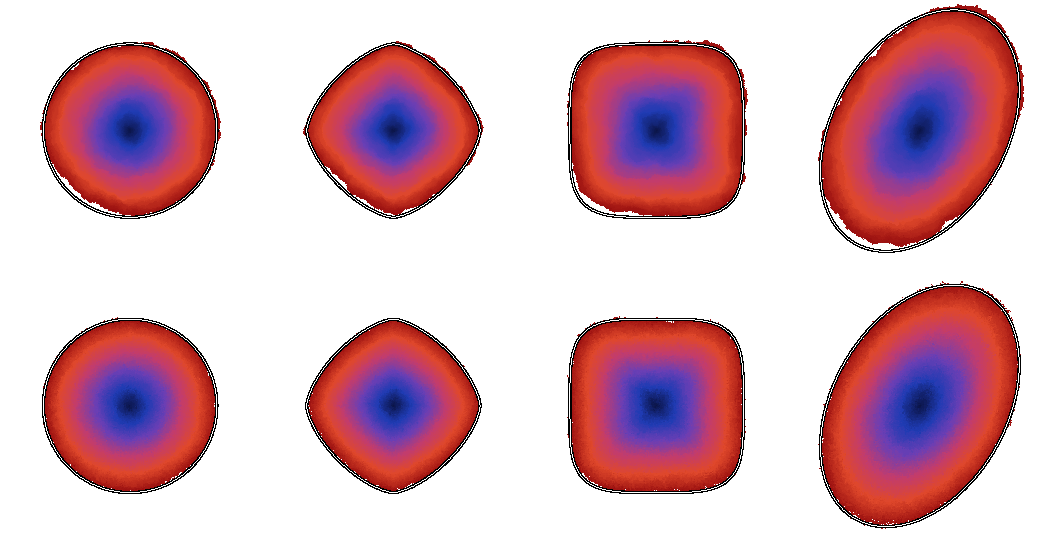
\includegraphics[width=\textwidth]{Figures/shapes_ranges.pdf}
\caption{Ranges $r_n^{-1}A_n$ for the Euclidean, $\ell^{3/2}$, $\ell^4$ and elliptical norms (left to right), at $n=10^9$. Top: $d=2$, $\drift=0.4$; bottom: $x_3=0$ sections for $d=3$, $\drift=0.25$. Curves mark unit balls; blue-to-red colors show $(t_x/n)^{\nf{1}{(d+1)}}$, with $t_x$ the first-departure time.}
\label{fig:ranges}
\end{figure}

\begin{figure}[t]
\centering
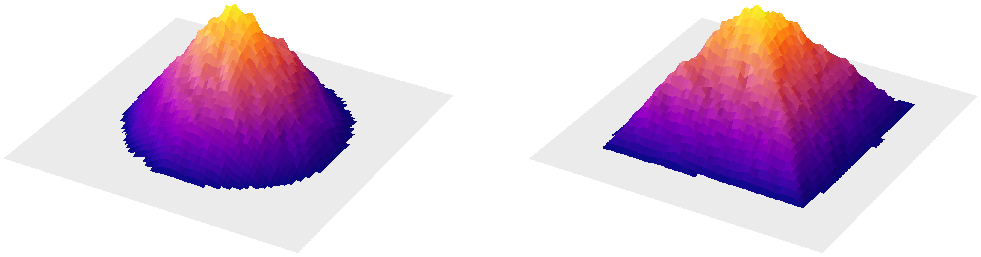
\includegraphics[width=\textwidth]{Figures/shapes_localtimes.pdf}
\caption{Local times $\ell_n(x)/(2d\drift r_n)$ over $x/r_n$ for the Euclidean norm (left) and $\ell^\infty$ (right): $d=2$, $n=10^{10}$, $\drift=0.4$. Heights average $75\times75$ and $69\times69$ blocks, respectively; gray marks unvisited blocks.}
\label{fig:profiles}
\end{figure}

\subsection{Strategy and key ideas}\label{sec:strategy}

The proof rests on an explicit potential. For a bounded measurable set~$D\subset\R^d$ and $y\in\R^d$, let
\begin{equation}\label{eq:potential-intro}
U_D(y)\coloneqq\frac{2\drift}{\omega_d}\int_D\frac{v}{|v|}\cdot\frac{v-y}{|v-y|^d}\dd v
\end{equation}
be the potential generated by the vector field~$-\drift v/|v|$ on~$D$. Integration along the rays from~$y$ shows that the potential of a ball is a cone: for every $\rho>0$ and every $y\in\R^d$,
\begin{equation}\label{eq:ballpotential-euclid}
U_{B(0,\rho)}(y)=2d\drift(\rho-|y|)_+\, .
\end{equation}
Replacing $v/|v|$ by~$\nabla\gauge(v)$ gives the cone $2d\drift(\rho-\gauge(y))_+$ for a ball of the norm (Lemma~\ref{lem:ballpotential}).

Dynkin's formula compares the local times with~$U_{D_n}$, up to a martingale and a smaller error. The obstacle is a thin extension of the range: its potential can be smaller than the martingale error. We combine two facts to exclude it. Local times vanish outside the range, and a walk can reach a distant site only by crossing the intervening region against its first-departure drift. The decisive comparison is at a contact point of the largest ball about the origin contained in~$D_n$: the potential is small there, and the excess outside the ball contributes nonnegatively.
\begin{enumerate}[label=\arabic*.,leftmargin=*]
\item \emph{Local times and the potential} (Section~\ref{sec:local}). Freedman's inequality controls the Dynkin martingales uniformly over sites and time intervals. Replacing the discrete drift sum by~$U_{D_n}$ costs $O(\log n)$, including for norms with corners; convexity controls the variation of subgradients across a cell (Lemma~\ref{lem:cell}).
\item \emph{Crossing and coarse bounds} (Section~\ref{sec:coarse}). The inward drift prevents the walk from crossing a region with few departures. This bounds its radius by the largest local time outside a ball. A first application gives a crude radius bound; the contact comparison then bounds those exterior local times, and a second application gives $\Rout(n)\asymp\max_x\ell_n(x)\asymp r_n$ and $|A_n|\asymp r_n^d$ (Proposition~\ref{prop:coarse}).
\item \emph{The limit shape} (Section~\ref{sec:norms}). At a contact point~$y_0$, Dynkin's formula at a neighboring site outside~$A_n$ bounds~$U_{D_n}(y_0)$ (Lemma~\ref{lem:contact}). Convexity makes the contribution of every excess point~$v$ at least $c(\gauge(v)-b)r_n^{-d}$, where $b$ is the radius of the largest norm ball in~$D_n$. The excess therefore has small potential, giving the conical local times; the quadratic martingale gives $b\approx r_n$. To exclude thin extensions for a norm with corners, we cross in the direction of the Euclidean projection onto the norm ball, whose normal has positive inner product with every subgradient at sites near the maximum in that direction.
\item \emph{The inner radius} (Section~\ref{sec:contact}). For the Euclidean norm, an excess point~$v$ contributes at least $c|v-y_0|^{2-d}/r_n$ at the contact point. This bounds the excess volume by~$Cr_n^{d-1}U_{D_n}(y_0)$ and sharpens the inner-radius estimate (Proposition~\ref{prop:inner}).
\item \emph{The outer radius} (Section~\ref{sec:outer}). We evaluate the potential beyond the outer radius, where the local time vanishes. The excess near the enclosing sphere contributes negatively; curvature bounds the positive contribution. These volume bounds control the local times outside the inner ball, and the crossing estimate gives the outer-radius bound (Proposition~\ref{prop:stronger-outer}). The same estimates give the uniform local-time bound.
\end{enumerate}
The conical profile determines the bracket limits, so the martingale central limit theorem and the law of the iterated logarithm give the limit laws of Section~\ref{sec:sharp}. Exponential martingales give the larger deviations needed for the lower bounds: one martingale controls the planar radii, and many weakly correlated martingales control the largest local time. The width uses the vector martingale $X_n+\drift\sum_{x\in A_n}x/|x|$. Cancellation inside the inner disk turns its order~$\sqrt n$ fluctuations into width fluctuations of order~$\sqrt{r_n}$; its two-dimensional Gaussian limit gives the small-ball bound. Figure~\ref{fig:dependence} records the dependencies.

\begin{figure}[t]
\centering
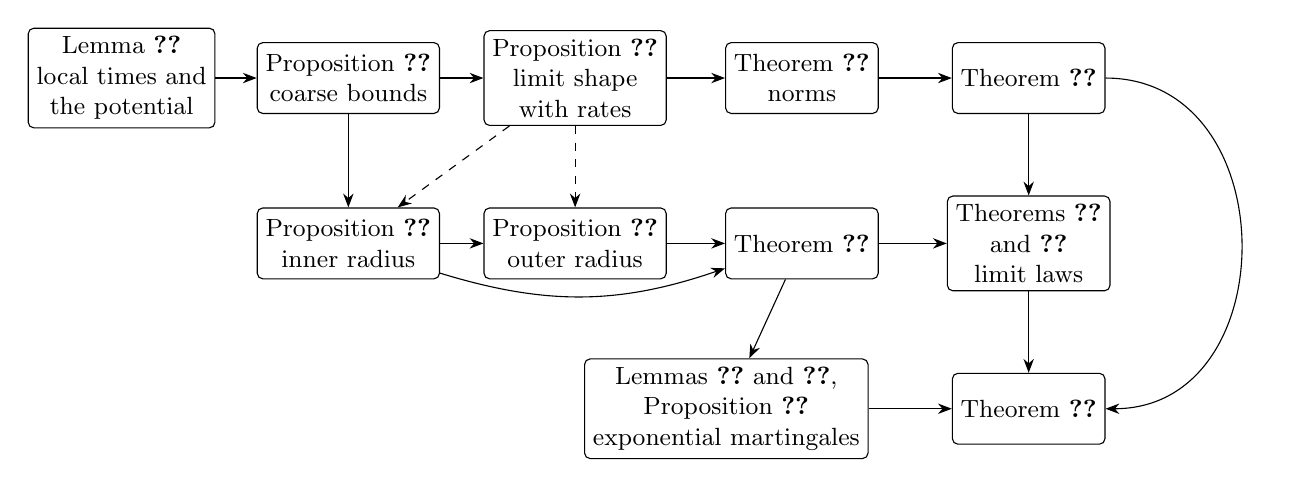
\begin{tikzpicture}[x=0.96cm,y=1cm,
  box/.style={draw,rounded corners=2pt,align=center,font=\small,
    inner sep=3pt,minimum height=0.9cm},
  arr/.style={-{Stealth[length=5pt]},thin}]
\node[box] (L) at (0,0) {Lemma~\ref{lem:local}\\ local times and\\ the potential};
\node[box] (P3) at (3,0) {Proposition~\ref{prop:coarse}\\ coarse bounds};
\node[box] (P4) at (6,0) {Proposition~\ref{prop:norm-shape}\\ limit shape\\ with rates};
\node[box] (TN) at (9,0) {Theorem~\ref{thm:norm-shape}\\ norms};
\node[box] (TA) at (12,0) {Theorem~\ref{thm:shape}};
\node[box] (P5) at (3,-2.1) {Proposition~\ref{prop:inner}\\ inner radius};
\node[box] (P6) at (6,-2.1) {Proposition~\ref{prop:stronger-outer}\\ outer radius};
\node[box] (TB) at (9,-2.1) {Theorem~\ref{thm:fluctuations}};
\node[box] (S8) at (12,-2.1) {Theorems~\ref{thm:moment-fluctuations}\\ and~\ref{thm:site-fluctuations}\\ limit laws};
\node[box] (S9) at (8,-4.2) {Lemmas~\ref{lem:exp-deviation} and~\ref{lem:separated-brackets},\\ Proposition~\ref{prop:bulk-profile}\\ exponential martingales};
\node[box] (TC) at (12,-4.2) {Theorem~\ref{thm:sharp}};
\draw[arr] (L) -- (P3);
\draw[arr] (P3) -- (P4);
\draw[arr] (P4) -- (TN);
\draw[arr] (TN) -- (TA);
\draw[arr] (P3) -- (P5);
\draw[arr] (P5) -- (P6);
\draw[arr] (P6) -- (TB);
\draw[arr] (P5) to[bend right=18] (TB);
\draw[arr,dashed] (P4) -- (P5);
\draw[arr,dashed] (P4) -- (P6);
\draw[arr] (TA) -- (S8);
\draw[arr] (TB) -- (S8);
\draw[arr] (TB) -- (S9);
\draw[arr] (S8) -- (TC);
\draw[arr] (S9) -- (TC);
\draw[arr] (TA.east) to[out=0,in=0,looseness=1.4] (TC.east);
\end{tikzpicture}
\caption{How the main results depend on each other; every result also uses Lemma~\ref{lem:local}. Propositions~\ref{prop:inner} and~\ref{prop:stronger-outer} concern the Euclidean norm, and the dashed arrows mean that Proposition~\ref{prop:inner} uses Lemma~\ref{lem:contact} and Proposition~\ref{prop:stronger-outer} uses Lemmas~\ref{lem:layer} and~\ref{lem:outer-crossing}, with other estimates of Sections~\ref{sec:coarse} and~\ref{sec:norms}, but neither uses the conclusion of Proposition~\ref{prop:norm-shape}. Theorem~\ref{thm:sharp}\,(i) uses Theorems~\ref{thm:fluctuations} and~\ref{thm:moment-fluctuations} and Lemma~\ref{lem:exp-deviation}, part~(ii) uses Theorem~\ref{thm:moment-fluctuations}, part~(iii) uses Proposition~\ref{prop:bulk-profile} and Lemmas~\ref{lem:exp-deviation} and~\ref{lem:separated-brackets}, and part~(iv) uses Lemma~\ref{lem:exp-deviation}, Proposition~\ref{prop:coarse} and Theorem~\ref{thm:shape}\,(i).}
\label{fig:dependence}
\end{figure}

The local times play the role of the divisible-sandpile odometer, compared with an explicit potential in~\citet{LevinePeres2009}. Martingales with a pole at an unvisited site and separate estimates against thin extensions also appear in the internal diffusion-limited aggregation bounds of~\citet*{JerisonLevineSheffield2012,JerisonLevineSheffield2013}. Our logarithmic lower bounds use the inner/outer deviation dichotomy of~\citet[Proposition~1.2]{AsselahGaudilliere2014}.

\subsection{Related work}\label{sec:related}

\citet{Kozma2013} reported recurrence of the walk excited to the center, citing unpublished work from 2006. \citet*{DemboHuangSidoravicius2014} described the manuscript of~\citet{Kozma2006CentrallyExcited} for a related walk in $d\geq3$, with drift~$-\drift x/\|x\|_1$ at the first visit to a site having an unvisited neighbor; \citet*{DemboHuangSidoravicius2014Growing} cited it for recurrence in every dimension. We take the name centrally excited random walk from its title. Its direction-dependent drift magnitude differs from our constant Euclidean drift. \citet*{BenjaminiDuminilCopinKozmaLucas2020} also recorded the predicted radius~$t^{\nf{1}{(d+1)}}$.

For the excited random walk with first-visit drift in a fixed direction, \citet*{BenjaminiWilson2003} proved transience in $d\geq2$ and positive lower speed in $d\geq4$. \citet{Kozma2003Speed,Kozma2005Speed} obtained positive lower speed in $d=3$ and $d=2$, and \citet{BerardRamirez2007} proved laws of large numbers and central limit theorems. \citet*{MenshikovPopovRamirezVachkovskaia2012} extended positive-speed results to uniformly elliptic walks with bounded jumps and uniformly positive first-visit drift in a fixed direction and zero drift at later visits. \citet{Zerner2005,Zerner2006} gave recurrence/transience criteria on~$\Z$ and strips for walks with multiple cookies. \citet*{AmirBenjaminiKozma2008} proved recurrence for a walk in the upper half of~$\Z^3$ that steps down at new sites. See~\citet{KosyginaZerner2013} for a survey.

The radius~$n^{\nf{1}{(d+1)}}$ and range size~$n^{\nf{d}{(d+1)}}$ are also predicted for once-reinforced walks with strong reinforcement~\citep{Beffara2011,ElboimKozma2026}, and supported by simulations~\citep{FosterGrassbergerPaczuski2009}; related predictions for self-attracting walks appear in~\citet{OrdemannBerkolaikoHavlinBunde2000,OrdemannEtAl2001}. For once-reinforced random walk on~$\Z^d$, $d\geq2$, \citet{BouRabeePeres2026ORRW} proved the lower bound~$cn^{\nf{d}{(d+1)}}$ on the expected range for every reinforcement parameter. The matching upper bound and limit shape remain conjectural. See~\citet{Pemantle2007} for reinforced processes.

\citet{DemboGroismanHuangSidoravicius2021} proved an averaging principle and shape theorem for growth models motivated by origin-excited and once-reinforced walks. Their simulations with inward first steps along a coordinate of largest absolute value or along all coordinates produced squares and diamonds. Our norm theorem proves these shapes for first-departure drifts opposite to subgradients of~$\|\cdot\|_\infty$ and~$\|\cdot\|_1$. For related continuum growth models, \citet*{DemboYang2025Flow,DemboYang2025KPZ} obtained limits described by geometric flow and regularized Kardar--Parisi--Zhang equations.

Internal diffusion-limited aggregation~\citep{LawlerBramsonGriffeath1992} and rotor-router aggregation~\citep{LevinePeres2009} have Euclidean ball limit shapes. The former has radius fluctuations of order at most $\log r$ in the plane and $(\log r)^{\nf12}$ in higher dimensions~\citep{JerisonLevineSheffield2012,JerisonLevineSheffield2013,AsselahGaudilliere2013,AsselahGaudilliere2013Polynomial}, and its rescaled fluctuations approach a variant of the Gaussian free field~\citep{JerisonLevineSheffield2014}. For the centrally excited walk, Theorem~\ref{thm:sharp} gives much larger planar radius and width fluctuations; the fixed-site covariance in Theorem~\ref{thm:site-fluctuations} is again expressed through the Green function. See~\citet*{LevinePeres2017} for aggregation models.

For Eulerian walkers~\citep{PriezzhevDharDharKrishnamurthy1996}, simulations suggested a circular planar range of radius of order~$t^{\nf13}$~\citep{KapriDhar2009}. \citet*{FlorescuLevinePeres2016} proved that every simple rotor walk on~$\Z^d$ visits at least $cn^{\nf{d}{(d+1)}}$ sites in $n$~steps. For clockwise planar rotors with independent uniform initial states, \citet*{BouRabeePeres2026} proved convergence of the rescaled range to a deterministic compact convex set; whether it is a disk remains open.

\subsection{Notation and conventions}\label{sec:notation}

\begin{itemize}
\item The Euclidean norm is $|x|$, and $\|x\|_p$ is the $\ell^p$~norm for $1\leq p\leq\infty$. The cardinality of a set~$A\subset\Z^d$ is~$|A|$, and the Lebesgue measure of a set~$D\subset\R^d$ is~$|D|$. The symmetric difference is~$\triangle$, and $t_+\coloneqq\max\{t,0\}$ and $s\vee t\coloneqq\max\{s,t\}$.
\item Let $u_x\coloneqq x/|x|$ for $x\in\R^d\setminus\{0\}$ and $u_0\coloneqq0$, and let $\xi(0)\coloneqq0$.
\item The letters $c>0$ and $C>0$ denote constants depending only on $d$, $\drift$ and the exponent~$p$ of the failure probability under discussion, and in Sections~\ref{sec:norm-setup}--\ref{sec:norms} also on the norm~$\gauge$, but not on the choice of the subgradients~$\xi(x)$; they may change from line to line. Every further dependence is stated, and a subscript on~$O$, as in~$O_y$, means that the implied constant also depends on~$y$. We write $a_n\asymp b_n$ if $c\leq a_n/b_n\leq C$, and $O_{\P}(a_n)$ for random variables~$Y_n$ such that $Y_n/a_n$ is tight.
\item The $\sigma$-field generated by $X_0,\ldots,X_j$ is~$\mathcal F_j$. For martingales $Z_1$ and~$Z_2$, the brackets $\langle Z_1\rangle_n$ and~$\langle Z_1,Z_2\rangle_n$ are the predictable quadratic variation and covariation through time~$n$.
\item The indicator that the step at time~$j$ is a first departure is $I_j\coloneqq\ind_{\{X_j\notin A_j\}}$, so that $\E(X_{j+1}-X_j\mid\mathcal F_j)=-\drift I_j\xi(X_j)$, where $\xi(x)=u_x$ for the Euclidean norm.
\item The function~$\widetilde\ell_n$ on~$\R^d$ equals $\ell_n(x)$ on~$C_x$ for every $x\in\Z^d$; it vanishes off~$D_n$.
\item All estimates concern integers~$n\geq2$, so that $\log n>0$. In a statement that holds with probability at least $1-Cn^{-p}$ for all sufficiently large~$n$, enlarging~$C$ makes it hold for every $n\geq2$.
\end{itemize}

\subsection*{Use of artificial intelligence}
The authors developed the main ideas of this work and directed its mathematical development. Throughout the project, the authors used large language models as research assistants: to explore specific questions arising in the proofs, to check the arguments and the cited results, and to audit drafts of the paper. The exposition, the simulations and the figures were produced with AI agents, primarily Claude (Anthropic), under the close supervision of the authors. The results of this paper have been formalized in Lean~4. The development covers every theorem, proposition and lemma of the paper, including the limit-shape theorem for walks with a norm, and assumes no cited result as a hypothesis: it also proves the martingale central limit theorem and Stout's law of the iterated logarithm, in the forms the paper uses. It states its exact coverage and every difference from this paper at \url{https://github.com/nitromannitol/Centrally-Excited-Random-Walk}. The authors take responsibility for the mathematical content and presentation of the paper.

\subsection*{Concurrent work}
A version of this manuscript containing our limit-shape and fluctuation results was recorded in our then-private \href{https://github.com/nitromannitol/Centrally-Excited-Random-Walk/commit/4a542809e64452751b0395544b9fe274122884d0}{GitHub repository} on 30 September 2026, before the independent preprint of \citet{Nguyen2026} appeared on 6 October 2026 (\url{https://arxiv.org/abs/2610.07724}). Nguyen proves convergence in probability, in Hausdorff distance, to an explicit $\ell^1$ ball in every dimension $d\geq2$. For his bias parameter $0<\theta<1$, the first-departure probabilities agree with ours for the $\ell^1$ norm, with $\drift=\theta/d$, away from the coordinate hyperplanes; the probabilities differ on these hyperplanes, and the limiting balls coincide. For our walk, we prove almost-sure shape and uniform local-time convergence for every norm, together with quantitative fluctuation bounds.

\subsection*{Acknowledgments}
The research of Y. Peres was supported by the National Natural Science Foundation of China grant RFIS-W2531011.

\section{Drifts given by a norm}\label{sec:norm-setup}

In this section we give the precise setting for a drift opposite to a subgradient of a norm and state the limit shape theorem in this setting, Theorem~\ref{thm:norm-shape}, of which Theorem~\ref{thm:shape} is the Euclidean case. We also prove the identity for the potential of a ball of the norm on which its proof rests (Lemma~\ref{lem:ballpotential}). Sections~\ref{sec:local}--\ref{sec:norms} work in this setting and prove Theorem~\ref{thm:norm-shape} at the end of Section~\ref{sec:norms}.

Let $\gauge$ be a norm on~$\R^d$, let $B_\gauge$ be its unit ball, and let $\partial\gauge(x)$ be the set of subgradients of~$\gauge$ at~$x$, as in Section~\ref{sec:norms-intro}; if $\gauge$ is differentiable at~$x$, then $\partial\gauge(x)=\{\nabla\gauge(x)\}$. At each site~$x\neq0$ fix $\xi(x)\in\partial\gauge(x)$, with coordinates~$\xi_i(x)$. The \defn{centrally excited random walk with norm~$\gauge$} moves like simple random walk, except that on its first departure from each site~$x\neq0$ it moves to $x\pm e_i$ with probability
\begin{equation}\label{eq:kernel}
\frac1{2d}\mp\frac\drift2\xi_i(x)
\qquad\text{for } 1\leq i\leq d\, .
\end{equation}
We assume that
\begin{equation}\label{eq:ellipticity}
\drift\max_{1\leq i\leq d}\gauge(e_i)<\frac1d\, .
\end{equation}
Every $\xi\in\partial\gauge(x)$ satisfies $\xi\cdot y\leq\gauge(y)$ for every~$y$, with equality at $y=x$ (Euler's relation); so $|\xi_i(x)|\leq\gauge(e_i)$, and~\eqref{eq:ellipticity} makes the probabilities~\eqref{eq:kernel} positive. The step at the first departure from~$x$ has conditional mean~$-\drift\xi(x)$, whose inner product with~$x$ is $-\drift\gauge(x)<0$. The Euclidean norm, with $\xi(x)=x/|x|$, gives the walk of Section~\ref{sec:introduction}, and then~\eqref{eq:ellipticity} reads $\drift<\nf1d$. Let
\begin{equation}\label{eq:radius-norm}
r_n\coloneqq\left(\frac{(d+1)n}{2d\drift|B_\gauge|}\right)^{\nf{1}{(d+1)}}\, ,
\end{equation}
which is~\eqref{eq:radius} when $\gauge$ is the Euclidean norm; the cone $2d\drift(r_n-\gauge(v))_+$ has integral~$n$ over~$\R^d$.

In Sections~\ref{sec:norm-setup}--\ref{sec:norms}, $\gauge$ is a norm, $\drift>0$ satisfies~\eqref{eq:ellipticity}, $r_n$ is given by~\eqref{eq:radius-norm}, and $U_D$ is the potential~\eqref{eq:potential-norm} defined below; at a point~$v\in\R^d$, $\nabla\gauge(v)$ is the gradient, which exists for almost every~$v$. Let $\Lambda_\gauge\coloneqq\max_{|u|=1}\gauge(u)$ and $c_\gauge\coloneqq\min_{|u|=1}\gauge(u)$; every $\xi\in\partial\gauge(x)$ satisfies $\xi\cdot x=\gauge(x)$ and $|\xi|\leq\Lambda_\gauge$. In Sections~\ref{sec:contact}--\ref{sec:lower}, $\gauge$ is the Euclidean norm, so that $\xi(x)=u_x$, $r_n$ is given by~\eqref{eq:radius}, and $U_D$ is the potential~\eqref{eq:potential-intro}.

\begin{theorem}[Limit shape for a norm]\label{thm:norm-shape}
Let $d\geq2$, let $\gauge$ be a norm on~$\R^d$, let $\xi(x)\in\partial \gauge(x)$ be chosen at the sites $x\in\Z^d\setminus\{0\}$, let $\drift>0$ satisfy~\eqref{eq:ellipticity}, and let $r_n$ be as in~\eqref{eq:radius-norm}. Then, almost surely, the centrally excited random walk with norm~$\gauge$ has the following properties.
\begin{enumerate}[label=\textup{(\roman*)}]
\item \underline{\emph{Shape}}: for every $0<\eta<1$ and all sufficiently large~$n$,
\begin{equation*}
\{x\in\Z^d:\gauge(x)<(1-\eta)r_n\}\subset A_n\subset\{x\in\Z^d:\gauge(x)<(1+\eta)r_n\}\, .
\end{equation*}
\item \underline{\emph{Local times}}: as $n\to\infty$,
\begin{equation*}
\frac1{r_n}\max_{x\in\Z^d}\bigl|\ell_n(x)-2d\drift(r_n-\gauge(x))_+\bigr|\longrightarrow0\, .
\end{equation*}
\item \underline{\emph{Recurrence}}: the walk visits every site of~$\Z^d$ infinitely often.
\end{enumerate}
\end{theorem}

Proposition~\ref{prop:norm-shape} gives rates: for every $p>0$ there is a constant $C(d,\drift,\gauge,p)$, not depending on the choice of~$\xi$, such that with probability at least $1-Cn^{-p}$ the maximum in part~(ii) is at most $Cr_n^{\nf56}(\log n)^{\nf16}$ if $d=2$ and $Cr_n^{\nf{d}{(d+1)}}(\log n)^{\nf{1}{(d+1)}}$ if $d\geq3$, and the inclusions of part~(i) hold with $\eta r_n$ replaced by $\log n$ times this bound on the maximum. Part~(i) gives $|A_n|/r_n^d\to|B_\gauge|$, and for the Euclidean norm Theorem~\ref{thm:fluctuations} gives smaller error bounds.

\subsection{The potential of a norm ball}\label{sec:ballpotential}

For a norm~$\gauge$, the potential~\eqref{eq:potential-intro} is defined with the gradient of~$\gauge$ in place of~$v/|v|$: for a bounded measurable set~$D\subset\R^d$ and $y\in\R^d$, let
\begin{equation}\label{eq:potential-norm}
U_D(y)\coloneqq\frac{2\drift}{\omega_d}\int_D\nabla\gauge(v)\cdot\frac{v-y}{|v-y|^d}\dd v
\end{equation}
be the potential generated by the vector field~$-\drift\nabla\gauge$ on~$D$; for the Euclidean norm it is~\eqref{eq:potential-intro}.

For every Lipschitz function~$f$ with compact support and every $y\in\R^d$,
\begin{equation}\label{eq:gradient-identity}
\int_{\R^d}\nabla f(v)\cdot\frac{v-y}{|v-y|^d}\dd v=-d\omega_df(y)\, .
\end{equation}
To prove it, write $v=y+tu$ with $t>0$ and $|u|=1$, so that $(v-y)|v-y|^{-d}\dd v=u\dd t\dd S(u)$. By Rademacher's and Fubini's theorems, for almost every~$u$ the Lipschitz function $t\mapsto f(y+tu)$ has derivative $\nabla f(y+tu)\cdot u$ for almost every $t>0$; this function vanishes for large~$t$, so its derivative integrates to $-f(y)$ over $t>0$, and the unit sphere has area $d\omega_d$.

\begin{lemma}[The potential of a norm ball]\label{lem:ballpotential}
Let $\gauge$ be a norm, let $\rho>0$, and let $y\in\R^d$. Then
\begin{equation}\label{eq:ballpotential}
U_{\{\gauge<\rho\}}(y)=2d\drift(\rho-\gauge(y))_+\, .
\end{equation}
\end{lemma}

\begin{proof}
The set $\{\gauge<\rho\}$ is bounded, and $\{\gauge=\rho\}$ has measure zero because $\gauge$ is homogeneous, so $\nabla(\rho-\gauge)_+=-\ind_{\{\gauge<\rho\}}\nabla \gauge$ almost everywhere. Applying~\eqref{eq:gradient-identity} to the Lipschitz function $f=(\rho-\gauge)_+$, which has compact support, proves the lemma.
\end{proof}

For the Euclidean norm, Lemma~\ref{lem:ballpotential} is the identity~\eqref{eq:ballpotential-euclid}.

\section{Local times and the potential}\label{sec:local}

In this section we prove Lemma~\ref{lem:local}, which bounds the local times on every time interval by the number of first departures in it and compares the local times with the potential~$U_{D_n}$. Dynkin's formula expresses each local time as~$U_{D_n}$ minus a martingale, up to an error term. We bound the bracket of this martingale by a weighted sum of the local times, and use convexity to bound the error from replacing the subgradients~$\xi(x)$ chosen at the sites by the gradient~$\nabla\gauge$ on the cells (Lemma~\ref{lem:cell}).

For integers~$0\leq s<t\leq n$, let
\begin{equation*}
M_{s,t}\coloneqq\max_{x\in\Z^d}\sum_{s\leq j<t}\ind_{\{X_j=x\}}
\qquad\text{and}\qquad
k_{s,t}\coloneqq\sum_{s\leq j<t}I_j\, .
\end{equation*}

\begin{lemma}\label{lem:local}
Let $p>0$. There exists $C(d,\drift,\gauge,p)<\infty$ such that, for every integer~$n\geq2$, the following estimates hold simultaneously with probability at least $1-Cn^{-p}$.
\begin{enumerate}[label=\textup{(\roman*)}]
\item \underline{\emph{Largest local time}}:
\begin{equation}\label{eq:M}
\max_{x\in\Z^d}\ell_n(x)\leq C|A_n|^{\nf{1}{d}}+C(\log n)^2\, .
\end{equation}
\item \underline{\emph{Local times on time intervals}}: for all integers~$0\leq s<t\leq n$,
\begin{equation}\label{eq:interval}
M_{s,t}\leq Ck_{s,t}^{\nf{1}{d}}+C(\log n)^2\, .
\end{equation}
\item \underline{\emph{Approximation by the potential}}: for every $y\in\R^d$ with $|y|\leq2n$,
\begin{equation}\label{eq:approx}
|\widetilde\ell_n(y)-U_{D_n}(y)|\leq C\log n+C\begin{cases}\bigl(\max_x\ell_n(x)\bigr)^{\nf12}\log n,&d=2,\\\bigl(\max_x\ell_n(x)\log n\bigr)^{\nf12},&d\geq3\end{cases}\, .
\end{equation}
\end{enumerate}
\end{lemma}

Once $\max_x\ell_n(x)\leq Cr_n$, as on the event of Proposition~\ref{prop:coarse}, the right side of~\eqref{eq:approx} is at most $C\sqrt{r_n}\log n=o(r_n)$.

\subsection{Dynkin's formula for the local times}\label{sec:dynkin}

Let $\Delta f(x)\coloneqq(2d)^{-1}\sum_{|e|=1}(f(x+e)-f(x))$, summed over the unit vectors $e\in\Z^d$, be the discrete Laplacian. For $d=2$, let $g$ be the potential kernel of simple random walk, normalized by $g(0)=0$. For $d\geq3$, let $g\coloneqq-G$, where the Green function~$G(x)$ is the expected number of visits to~$x$ by simple random walk from the origin. In both cases $\Delta g=\ind_{\{0\}}$; for $d=2$ see \citet*[Proposition~4.4.2]{LawlerLimic2010}. By \citet[Theorems~4.3.1 and~4.4.4]{LawlerLimic2010}, as $|x|\to\infty$,
\begin{equation}\label{eq:kernel-asymptotics}
g(x)=\begin{dcases}
\frac2\pi\log|x|+c_g+O(|x|^{-2}),&d=2,\\
-\frac{2}{(d-2)\omega_d}|x|^{2-d}+O(|x|^{-d}),&d\geq3
\end{dcases}\, ,
\end{equation}
where $c_g$ is a constant. Let $\bar\nabla g(x)$ be the vector with coordinates $(g(x+e_i)-g(x-e_i))/2$ for $1\leq i\leq d$. Then
\begin{equation}\label{eq:gradient}
\bar\nabla g(x)=\frac2{\omega_d}\frac{x}{|x|^d}+O(|x|^{-d})
\quad\text{and}\quad
|g(x+e)-g(x)|\leq C(1+|x|)^{1-d}\, ,
\end{equation}
the first for $x\neq0$, the second for every $x\in\Z^d$ and every unit vector $e\in\Z^d$; see \citet[Corollaries~4.3.3 and~4.4.5]{LawlerLimic2010}.

For $f\colon\Z^d\to\R$ with bounded nearest-neighbor increments, let
\begin{equation*}
\mathcal M^f_t\coloneqq f(X_t)-f(X_0)-\sum_{j<t}\E\bigl(f(X_{j+1})-f(X_j)\bigm|\mathcal F_j\bigr)
\end{equation*}
be the martingale in Dynkin's formula for~$f$. By~\eqref{eq:kernel}, the conditional expectation in the sum is $\Delta f(X_j)-\drift I_j\xi(X_j)\cdot\bar\nabla f(X_j)$, with $\bar\nabla f$ defined like~$\bar\nabla g$. For $y\in\Z^d$ write $g_y\coloneqq g(\cdot-y)$ and $\mathcal M^y\coloneqq\mathcal M^{g_y}$. Since $\Delta g_y=\ind_{\{y\}}$ and each site of~$A_n$ has its first departure before time~$n$,
\begin{equation}\label{eq:dynkin}
\ell_n(y)=g(X_n-y)-g(-y)
+\drift\sum_{x\in A_n}\xi(x)\cdot\bar\nabla g(x-y)-\mathcal M_n^y\, .
\end{equation}
The difference $g(X_n-y)-g(-y)$ is $O(\log n)$ for $d=2$ and $O(1)$ for $d\geq3$, uniformly over $y\in\Z^d$ with $|y|\leq3n$. By~\eqref{eq:gradient}, the increments of~$\mathcal M^y$ are bounded, and
\begin{equation}\label{eq:bracket}
\langle\mathcal M^y\rangle_n\leq CW_y,\qquad\text{where}\quad
W_y\coloneqq\sum_{x\in\Z^d}\ell_n(x)(1+|x-y|)^{2-2d}\, .
\end{equation}

\begin{lemma}\label{lem:freedman}
Let $p>0$. There exists $C(p)<\infty$ such that the following holds for every integer~$n\geq2$ and every real martingale~$Z$ whose increments have absolute value at most~$1$: with probability at least $1-Cn^{-p}$,
\begin{equation}\label{eq:freedman}
|Z_n-Z_0|\leq C\bigl(\sqrt{\langle Z\rangle_n\log n}+\log n\bigr)\, .
\end{equation}
\end{lemma}

\begin{proof}
Apply \citet*[Theorem~1.6]{Freedman1975} on the dyadic intervals for~$\langle Z\rangle_n$, with thresholds $C(p)(\sqrt{2^i\log n}+\log n)$. Each interval has failure probability at most $2n^{-p-1}$. Since $\langle Z\rangle_n\leq n$, a union bound over $O(\log n)$ intervals proves~\eqref{eq:freedman}.
\end{proof}

We apply Lemma~\ref{lem:freedman} to constant multiples of possibly stopped martingales, with union bounds over polynomially many deterministic sites and time intervals; the resulting estimates then hold also at sites and intervals that depend on the path.

Let $\mu$ be the distributional Laplacian of~$\gauge$ on~$\R^d$, so that $\int\phi\dd\mu=\int \gauge(v)\sum_{i=1}^d\partial_i^2\phi(v)\dd v$ for every smooth compactly supported function~$\phi$ on~$\R^d$. The distributional Laplacian~$\mu$ is a positive Radon measure, because the smooth convex functions obtained by mollifying~$\gauge$ have nonnegative Laplacian. For $y\in\R^d$ and $R>0$, let $\phi$ be smooth with $0\leq\phi\leq1$, $\phi=1$ on~$B(y,R)$, support in~$B(y,2R)$ and $|\nabla\phi|\leq2/R$. Integrating by parts and using $|\nabla \gauge|\leq\Lambda_\gauge$ gives
\begin{equation}\label{eq:hessian-growth}
\mu(B(y,R))\leq\int\phi\dd\mu=-\int\nabla \gauge\cdot\nabla\phi\leq2^{d+1}\omega_d\Lambda_\gauge R^{d-1}\, .
\end{equation}

\begin{lemma}\label{lem:cell}
There exists $C(d)<\infty$ such that, for every $x\in\Z^d$,
\begin{equation*}
\int_{C_x}|\nabla \gauge(v)-\xi(x)|\dd v\leq C\mu\bigl(B(x,6\sqrt d)\bigr)\, .
\end{equation*}
\end{lemma}

\begin{proof}
The vector $\xi(x)$ is a subgradient of~$\gauge$ at~$x$; for $x=0$, where $\xi(0)=0$, this holds because $\gauge\geq0$. So $h(v)\coloneqq \gauge(v)-\gauge(x)-\xi(x)\cdot(v-x)$ is convex and nonnegative, $h(x)=0$, $\nabla h=\nabla \gauge-\xi(x)$ almost everywhere, and the distributional Laplacian of~$h$ is~$\mu$. At every point~$v$ where $h$ is differentiable, convexity of $s\mapsto h(v+se_i)$ and $h\geq0$ give $|\partial_ih(v)|\leq h(v+e_i)+h(v-e_i)$. The cells $C_{x\pm e_i}$ are disjoint and lie in~$B(x,A)$, where $A\coloneqq2\sqrt d$, so integrating over~$C_x$ and summing over~$i$ gives
\begin{equation*}
\int_{C_x}|\nabla h(v)|\dd v\leq\int_{B(x,A)}h(v)\dd v\, .
\end{equation*}
Let $h_r$ be the convolution of~$h$ with a smooth mollifier supported in~$B(0,r)$, where $0<r<A$. For a unit vector~$u$, the derivative of the convex function $s\mapsto h_r(x+su)$ is nondecreasing, so $h_r(x+su)\leq h_r(x)+s\bigl(u\cdot\nabla h_r(x+2Au)\bigr)$ for $0\leq s\leq A$. The Laplacian of~$h_r$ is the convolution of~$\mu$ with the mollifier, so by the divergence theorem the average of $u\cdot\nabla h_r(x+2Au)$ over unit vectors~$u$ is at most $C\mu(B(x,2A+r))$. Integrating in polar coordinates gives $\int_{B(x,A)}h_r\leq\omega_dA^dh_r(x)+C\mu(B(x,3A))$. Letting $r\to0$, and using that $h_r\to h$ locally uniformly and $h(x)=0$, proves the lemma.
\end{proof}

\begin{proof}[Proof of Lemma~\ref{lem:local}]
\emph{Step 1: The martingales on time intervals.} Let $y\in\Z^d$ with $|y|\leq3n$. Every site visited before time~$n$ lies within distance~$4n$ of~$y$, and the weights $(1+|x-y|)^{2-2d}$ of the sites~$x$ with $|x-y|\leq4n$ sum to $O(\log n)$ for $d=2$ and $O(1)$ for $d\geq3$. So $\langle\mathcal M^y\rangle_t-\langle\mathcal M^y\rangle_s$ is at most $CM_{s,t}$ times the sum of these weights. Lemma~\ref{lem:freedman} for the martingales $j\mapsto\mathcal M^y_{(s+j)\wedge t}-\mathcal M^y_s$, with a union bound over the $O(n^{d+2})$ pairs of an interval and a site~$y$, gives an event of probability at least $1-Cn^{-p}$ on which, for all integers~$0\leq s<t\leq n$ and all $y\in\Z^d$ with $|y|\leq3n$,
\begin{equation}\label{eq:interval-mart}
|\mathcal M_t^y-\mathcal M_s^y|\leq C\log n+C\begin{cases}\sqrt{M_{s,t}}\log n,&d=2,\\\sqrt{M_{s,t}\log n},&d\geq3\end{cases}\, .
\end{equation}
We work on this event.

\emph{Step 2: Local times on time intervals.} For every $y\in\R^d$ and every set of $k$~lattice sites, the sum of $(1+|x-y|)^{1-d}$ over the set is at most $Ck^{\nf{1}{d}}$, since it is largest for the $k$~sites nearest to~$y$. Subtract~\eqref{eq:dynkin} with $s$ in place of~$n$ from~\eqref{eq:dynkin} with $t$ in place of~$n$, so that the left side becomes the number of departures from~$y$ at the times $s\leq j<t$, and maximize over the sites~$y$ with $|y|\leq3n$, which include all sites visited before time~$n$. The differences of the terms $g(X_t-y)$ and $g(X_s-y)$ contribute $O(\log n)$, and~\eqref{eq:interval-mart} bounds the martingale terms. The difference of the sums over $A_t$ and~$A_s$ runs over the $k_{s,t}$ sites of $A_t\setminus A_s$, so by the bound above and~\eqref{eq:gradient} it is at most $Ck_{s,t}^{\nf{1}{d}}$. Young's inequality absorbs the term with~$\sqrt{M_{s,t}}$, which proves~\eqref{eq:interval}. Taking $s=0$ and $t=n$ gives~\eqref{eq:M}, since $M_{0,n}=\max_x\ell_n(x)$ and $k_{0,n}=|A_n|$.

\emph{Step 3: Comparison with the potential.} Let $y\in\Z^d$ with $|y|\leq3n$. By~\eqref{eq:dynkin}, the bound on $g(X_n-y)-g(-y)$ and~\eqref{eq:interval-mart} with $s=0$ and $t=n$, the local time~$\ell_n(y)$ differs from $\drift\sum_{x\in A_n}\xi(x)\cdot\bar\nabla g(x-y)$ by at most the right side of~\eqref{eq:approx}. The summand at $x=y$ vanishes because $\bar\nabla g(0)=0$. For $x\neq y$, replace $\bar\nabla g(x-y)$ by $(\nf{2}{\omega_d})(x-y)/|x-y|^d$; by~\eqref{eq:gradient}, the errors sum to at most $C\sum_{|x|\leq n}(1+|x-y|)^{-d}\leq C\log n$. Replacing each kernel value by its average over the cell~$C_x$ also changes the sum by at most $C\log n$: for cells at distance at least one from~$y$ each error is $O((1+|x-y|)^{-d})$, and the cells near~$y$, including $C_y$ if $y\in A_n$, contribute $O(1)$ because $|v-y|^{1-d}$ is locally integrable. The last replacement, of $\xi(x)$ by $\nabla \gauge(v)$ for $v\in C_x$, changes the sum by at most a constant times
\begin{equation*}
\sum_{x\in A_n}\int_{C_x}|v-y|^{1-d}|\xi(x)-\nabla \gauge(v)|\dd v\, .
\end{equation*}
The terms with $|x-y|\leq8\sqrt d$ contribute $O(1)$, because $|\xi(x)|$ and $|\nabla \gauge(v)|$ are at most~$\Lambda_\gauge$ and $|v-y|^{1-d}$ is locally integrable. If $|x-y|>8\sqrt d$, then $|v-y|\geq|x-y|/2$ for $v\in C_x$, and $|x-y|/4\leq|z-y|\leq2|x-y|$ for $z\in B(x,6\sqrt d)$; so Lemma~\ref{lem:cell} bounds the summand of~$x$ in the last display by $C\int_{B(x,6\sqrt d)}|z-y|^{1-d}\dd\mu(z)$. Each point of~$\R^d$ lies in at most $C$ of the balls $B(x,6\sqrt d)$ with $x\in\Z^d$, and those with $|x|\leq n$ and $|x-y|>8\sqrt d$ lie in $\{z:1\leq|z-y|\leq8n\}$. So the terms with $|x-y|>8\sqrt d$ contribute at most $C\int_{\{1\leq|z-y|\leq8n\}}|z-y|^{1-d}\dd\mu(z)\leq C\log n$, because~\eqref{eq:hessian-growth} bounds the integral over each of the $O(\log n)$ annuli $\{2^k\leq|z-y|<2^{k+1}\}$ by a constant. After the three replacements the sum $\drift\sum_{x\in A_n}\xi(x)\cdot\bar\nabla g(x-y)$ has become~$U_{D_n}(y)$, which proves~\eqref{eq:approx} for $y\in\Z^d$ with $|y|\leq3n$.

Finally, for $y\in\R^d$ with $|y|\leq2n$, let $z$ be the site with $y\in C_z$. Then $\widetilde\ell_n(y)=\ell_n(z)$, and splitting the integral~\eqref{eq:potential-norm} at $|v-z|=2\sqrt d$, as for the cell averages, gives $|U_{D_n}(y)-U_{D_n}(z)|\leq C\log n$. This proves~\eqref{eq:approx}.
\end{proof}

For every $p>0$, Lemma~\ref{lem:freedman} and~\eqref{eq:bracket} give, with probability at least $1-Cn^{-p}$, simultaneously for all $y\in\Z^d$ with $|y|\leq3n$,
\begin{equation}\label{eq:localmart}
|\mathcal M_n^y|\leq C\bigl(\sqrt{W_y\log n}+\log n\bigr)\, .
\end{equation}
The deterministic replacements in Step~3 of the proof of Lemma~\ref{lem:local} give, for every $y\in\Z^d$ with $|y|\leq3n$,
\begin{equation}\label{eq:pointwise}
\ell_n(y)=U_{D_n}(y)-\mathcal M_n^y+O(\log n)\, ,
\end{equation}
and splitting the integrals defining $U_{D_n}(y)$ and $U_{D_n}(z)$ at distance~$2\sqrt d$ from~$y$ and~$z$, as in that proof, gives, for all $y,z\in\R^d$ with $|y-z|\leq\sqrt d$ and $|y|,|z|\leq3n$,
\begin{equation}\label{eq:cellmodulus}
|U_{D_n}(y)-U_{D_n}(z)|\leq C\log n\, .
\end{equation}

\subsection{Bounds on the potential}\label{sec:potential-bounds}

The potential of a set is bounded by its volume, and by the width of a shell of~$\gauge$ that contains it. Let $D\subset\R^d$ be a bounded measurable set. For every $y\in\R^d$, the integral of $|v-y|^{1-d}$ over~$D$ is at most its integral over the ball of volume~$|D|$ centered at~$y$, which is $C|D|^{\nf{1}{d}}$; since $|\nabla \gauge|\leq\Lambda_\gauge$, there exists $C(d,\gauge)<\infty$ such that
\begin{equation}\label{eq:potential-bound}
\sup_{y\in\R^d}|U_D(y)|\leq C\drift|D|^{\nf{1}{d}}\, .
\end{equation}
The function~$U_D$ is continuous, because it is the convolution of the bounded, compactly supported vector field~$\ind_D\nabla\gauge$ with a kernel that is the sum of an integrable function and a bounded one. We write $\dd S$ for surface measure on a sphere.

Convexity of~$\gauge$ along lines bounds the potential of a set that lies between two balls of~$\gauge$ about the origin.

\begin{lemma}\label{lem:layer}
Let $b\geq0$ and $a>0$, and let $D$ be a measurable subset of $\{v\in\R^d:b\leq \gauge(v)\leq b+a\}$. Then
\begin{equation*}
\sup_{y\in\R^d}|U_D(y)|\leq2d\drift a\, .
\end{equation*}
\end{lemma}

\begin{proof}
Fix $y\in\R^d$, write $v=y+tu$ with $t>0$ and $|u|=1$, and let $h_u(t)\coloneqq \gauge(y+tu)$. As in the proof of~\eqref{eq:gradient-identity}, for almost every~$u$ the function~$h_u$ has derivative $\nabla \gauge(y+tu)\cdot u$ for almost every $t>0$, so
\begin{equation*}
U_D(y)=\frac{2\drift}{\omega_d}\int_{\{|u|=1\}}\int_0^\infty\ind_D(y+tu)h_u'(t)\dd t\dd S(u)\, .
\end{equation*}
Since $h_u$ is convex, there is $t_0\in[0,\infty]$ such that $h_u$ is nonincreasing on~$[0,t_0]$ and nondecreasing on~$[t_0,\infty)$. On each of these intervals, the change of variables $s=h_u(t)$ bounds the integral of $\ind_{[b,b+a]}(h_u(t))|h_u'(t)|$ by~$a$. Since $0\leq\ind_D(y+tu)\leq\ind_{[b,b+a]}(h_u(t))$, and $h_u'\leq0$ on the first interval and $h_u'\geq0$ on the second, the inner integral lies in~$[-a,a]$. Since the unit sphere has area~$d\omega_d$, it follows that $|U_D(y)|\leq(2\drift/\omega_d)\,d\omega_d\,a=2d\drift a$, which proves the lemma; by Lemma~\ref{lem:ballpotential}, equality holds at $y=0$ when $D=\{b\leq \gauge<b+a\}$.
\end{proof}

\section{Coarse bounds on the range and the local times}\label{sec:coarse}

We prove that, with high probability, $|A_n|$ has order~$r_n^d$, and $\Rout(n)=\max_{j\leq n}|X_j|$ and the largest local time have order~$r_n$ (Proposition~\ref{prop:coarse}). The drift at first departures opposes the crossing of a region with few visited sites, and~\eqref{eq:interval} bounds the time spent there. The crossing argument of Section~\ref{sec:crossing}, which rests on these two facts, bounds $\Rout(n)$, for every $a\geq0$, by $a/c_\gauge$ plus $C\log n$ times one plus the largest local time at the sites~$x$ with $\gauge(x)\geq a$ (inequality~\eqref{eq:euclid-crossing}). By Lemma~\ref{lem:local}, the largest local time is of order at most~$|A_n|^{\nf1d}$, so $\Rout(n)\leq C|A_n|^{\nf1d}\log n$. The potential at a point where the boundary of the largest ball of~$\gauge$ in~$D_n$ meets the closure of a cell disjoint from~$D_n$ (Section~\ref{sec:largest-ball}) then shows that the local times outside this ball are much smaller than $|A_n|^{\nf1d}/\log n$, so that $\Rout(n)\leq C|A_n|^{\nf1d}$, and that the local times are close to a cone, whose integral bounds~$|A_n|$.

\begin{proposition}\label{prop:coarse}
Let $p>0$. There exist $c(d,\drift,\gauge,p)>0$ and $C(d,\drift,\gauge,p)<\infty$ such that, for every integer~$n\geq2$, with probability at least $1-Cn^{-p}$,
\begin{equation*}
cr_n^d\leq|A_n|\leq Cr_n^d,\qquad
cr_n\leq\max_{x\in\Z^d}\ell_n(x)\leq Cr_n,\qquad
cr_n\leq\Rout(n)\leq Cr_n\, .
\end{equation*}
\end{proposition}

\subsection{Crossing a region with few visited sites}\label{sec:crossing}

A crossing against the drift requires a large increment of the martingale
\begin{equation}\label{eq:vector-def}
Z_t\coloneqq X_t+\drift\sum_{j<t}I_j\xi(X_j)\, ,
\end{equation}
which takes values in~$\R^d$ and has bounded increments. Azuma's inequality in each coordinate and a union bound over the pairs $s<t$ give, for every $p>0$, with probability at least $1-Cn^{-p}$,
\begin{equation}\label{eq:vector}
|Z_t-Z_s|\leq C\sqrt{(t-s)\log n}
\qquad\text{for } 0\leq s<t\leq n\, .
\end{equation}

\begin{lemma}\label{lem:crossing}
On the event in~\eqref{eq:vector}, with the constant~$C$ of~\eqref{eq:vector}, the following holds for every unit vector~$u$ and all integers $0\leq s<t\leq n$. If $u\cdot\xi(X_j)\geq0$ at every first departure time~$j$ with $s\leq j<t$, then
\begin{equation*}
u\cdot(X_t-X_s)\leq C\sqrt{(t-s)\log n}\, .
\end{equation*}
\end{lemma}

\begin{proof}
By~\eqref{eq:vector-def}, $u\cdot(X_t-X_s)=u\cdot(Z_t-Z_s)-\drift\sum_{s\leq j<t}I_ju\cdot\xi(X_j)\leq|Z_t-Z_s|$, and~\eqref{eq:vector} bounds the right side.
\end{proof}

The martingales of the functions $(q\cdot x-a)_+$ bound the number of sites~$x\in A_n$ at which $q\cdot x$ exceeds a given level (Step~2 of the proof of Lemma~\ref{lem:outer-crossing}); we bound them simultaneously for all vectors~$q$ in a finite deterministic set, because $q$ will depend on the path. For $q\in\R^d$ and $a\in\R$, let $\mathcal M^{q,a}$ be the martingale~$\mathcal M^f$ of Section~\ref{sec:dynkin} with $f(x)=(q\cdot x-a)_+$. If $|q|\leq\Lambda_\gauge$, then one step changes $q\cdot X_j$ by at most~$\Lambda_\gauge$, so the increments of~$\mathcal M^{q,a}$ are at most~$C$, and the bracket of~$\mathcal M^{q,a}$ through time~$n$ is at most $C\sum_{x:q\cdot x>a-\Lambda_\gauge}\ell_n(x)$, because $f$ is constant on $x$ and its neighbors unless $q\cdot x>a-\Lambda_\gauge$. Fix $p>0$. Lemma~\ref{lem:freedman} and a union bound over the $O(n^{d+1})$ pairs~$(q,a)$ with $q=\Lambda_\gauge u_x$ for some $x\in\Z^d$ with $0<|x|\leq n$ and $a\in\Lambda_\gauge\Z\cap[0,\Lambda_\gauge n]$ give, with probability at least $1-Cn^{-p}$, simultaneously for all these pairs,
\begin{equation}\label{eq:linear-mart}
|\mathcal M^{q,a}_n|\leq C\biggl(\sqrt{\log n\sum_{x:q\cdot x>a-\Lambda_\gauge}\ell_n(x)}+\log n\biggr)\, .
\end{equation}

\begin{lemma}\label{lem:outer-crossing}
Let $\alpha>0$. There exists $C(d,\drift,\gauge,\alpha,p)<\infty$ with the following property. Let $q\in\R^d$ satisfy $|q|\leq\Lambda_\gauge$, and consider a path of the walk that satisfies~\eqref{eq:vector}, and~\eqref{eq:linear-mart} for this~$q$ and every $a\in\Lambda_\gauge\Z\cap[0,\Lambda_\gauge n]$. Let $x_*$ be one of the sites $X_0,\ldots,X_n$ with $q\cdot X_j\leq T\coloneqq q\cdot x_*$ for $0\leq j\leq n$, and let $h>0$ be such that $q\cdot\xi(X_j)\geq\alpha$ for every $0\leq j\leq n$ with $q\cdot X_j>T-h$. For $b\geq0$ let $L_b\coloneqq1+\max\{\ell_n(x):x\in\Z^d,\ q\cdot x\geq b\}$. Then every $b\geq0$ satisfies
\begin{equation}\label{eq:outer-crossing}
T\leq\max\{T-h,b\}+CL_b\log n\, .
\end{equation}
\end{lemma}

\begin{proof}
Fix $b\geq0$. Steps~1--3 show that few sites of~$A_n$ lie where $q\cdot x$ exceeds a level slightly above $\max\{T-h,b\}$, and Step~4 shows that the walk cannot reach~$x_*$ through so few sites.

\emph{Step 1: Local times and drift beyond a level.} For $a\in\R$ let $\mathcal N(a)$ be the number of sites $x\in A_n$ with $q\cdot x>a$. Let $a_0$ be the least element of~$\Lambda_\gauge\Z$ that is at least $\max\{T-h,b+\Lambda_\gauge\}$. If $a\geq a_0$, then:
\begin{enumerate}[label=\textup{(\alph*)}]
\item every $x\in A_n$ with $q\cdot x>a-\Lambda_\gauge$ satisfies $q\cdot x>b$, so $\ell_n(x)<L_b$;
\item every $x\in A_n$ with $q\cdot x>a$ satisfies $q\cdot x>T-h$, so $q\cdot\xi(x)\geq\alpha$ by hypothesis.
\end{enumerate}

\emph{Step 2: Comparison of neighboring levels.} Since $|q|\leq\Lambda_\gauge$ and $|x_*|\leq n$, we have $T\leq\Lambda_\gauge n$, and $\mathcal N(a)=0$ for $a\geq T$; so it suffices to consider levels $a\leq\Lambda_\gauge n$. Fix $a\in\Lambda_\gauge\Z$ with $a_0\leq a\leq\Lambda_\gauge n$, and put $\phi(x)\coloneqq(q\cdot x-a)_+$. Dynkin's formula gives
\begin{equation*}
\phi(X_n)=\sum_{j<n}\bigl[\Delta\phi(X_j)-\drift I_j\xi(X_j)\cdot\bar\nabla\phi(X_j)\bigr]+\mathcal M^{q,a}_n\, .
\end{equation*}
If $q\cdot x\geq a+\Lambda_\gauge$, then $\phi$ is linear on $x$ and its neighbors, because $|q|\leq\Lambda_\gauge$, so $\Delta\phi(x)=0$ and $\bar\nabla\phi(x)=q$, and by~(b) the drift term at the first departure from~$x$ is at most $-\drift\alpha$; at later departures from~$x$ the drift term vanishes. If $q\cdot x\leq a-\Lambda_\gauge$, then $\phi$ vanishes at~$x$ and its neighbors. At the remaining sites, $|\Delta\phi|$ and $|\bar\nabla\phi|$ are at most~$C$. Since $\phi(X_n)\geq0$ and $\phi(X_0)=0$, properties~(a) and~(b) and~\eqref{eq:linear-mart} give
\begin{equation*}
\drift\alpha\mathcal N(a+\Lambda_\gauge)
\leq CL_b|\{x\in A_n:|q\cdot x-a|<\Lambda_\gauge\}|
+C\sqrt{L_b\mathcal N(a-\Lambda_\gauge)\log n}+C\log n\, .
\end{equation*}
Hence, for every $a\in\Lambda_\gauge\Z$ with $a\geq a_0$,
\begin{equation}\label{eq:norm-linear}
\mathcal N(a+\Lambda_\gauge)\leq CL_b[\mathcal N(a-\Lambda_\gauge)-\mathcal N(a+\Lambda_\gauge)]
+C\sqrt{L_b\mathcal N(a-\Lambda_\gauge)\log n}+C\log n\, .
\end{equation}

\emph{Step 3: Iteration over the levels.} Set $N_k\coloneqq\mathcal N(a_0-\Lambda_\gauge+2k\Lambda_\gauge)$. Young's inequality in~\eqref{eq:norm-linear} gives $N_{k+1}\leq(1-c/L_b)N_k+C\log n$. Since $N_0\leq n$, iteration to $k=\lceil L_b\log n/c\rceil$ gives, with $\bar a\coloneqq a_0-\Lambda_\gauge+2k\Lambda_\gauge$,
\begin{equation}\label{eq:norm-small}
a_0\leq\bar a\leq a_0+CL_b\log n\qquad\text{and}\qquad\mathcal N(\bar a)\leq CL_b\log n\, .
\end{equation}

\emph{Step 4: The bound on~$T$.} If $T\leq\bar a+\Lambda_\gauge$, then $T-a_0\leq CL_b\log n$ by~\eqref{eq:norm-small}. Otherwise, $q\neq0$ because $T>0$; let $\sigma$ be the first $j\leq n$ with $X_j=x_*$, and let $s\coloneqq1+\max\{j<\sigma:q\cdot X_j\leq\bar a\}$. The set $\{j<\sigma:q\cdot X_j\leq\bar a\}$ contains~$0$ because $q\cdot X_0=0\leq\bar a$, and $s<\sigma$ because $T>\bar a+\Lambda_\gauge$ and each step changes $q\cdot X_j$ by at most~$\Lambda_\gauge$. For $s\leq j<\sigma$, the site~$X_j$ belongs to~$A_n$ and satisfies $q\cdot X_j>\bar a\geq a_0$, so~(b) gives $q\cdot\xi(X_j)>0$. By~\eqref{eq:norm-small} and~(a), at most $CL_b\log n$ distinct sites occur among $X_s,\ldots,X_{\sigma-1}$, each with local time less than~$L_b$, so $\sigma-s\leq CL_b^2\log n$. Lemma~\ref{lem:crossing} with $u=q/|q|$ and $t=\sigma$ gives $q\cdot(X_\sigma-X_s)\leq C\sqrt{(\sigma-s)\log n}\leq CL_b\log n$. Since $q\cdot X_\sigma=T$ and $q\cdot X_s\leq\bar a+\Lambda_\gauge$, the bound $T-a_0\leq CL_b\log n$ holds in this case as well. As $a_0\leq\max\{T-h,b+\Lambda_\gauge\}+\Lambda_\gauge$ and $L_b\geq1$, this proves~\eqref{eq:outer-crossing}.
\end{proof}

Let $x_*$ be one of the sites $X_0,\ldots,X_n$ with $|x_*|=\Rout(n)$, so that $x_*\neq0$ and $|x_*|\leq n$. Let $q\coloneqq\Lambda_\gauge u_{x_*}$ and $T\coloneqq q\cdot x_*=\Lambda_\gauge\Rout(n)$, so that $q\cdot X_j\leq\Lambda_\gauge|X_j|\leq T$ for $0\leq j\leq n$, and let $\theta\coloneqq c_\gauge^2/(8\Lambda_\gauge^2)$. If $q\cdot X_j>(1-\theta)T$, then $X_j\neq0$ and $u_{x_*}\cdot u_{X_j}>(1-\theta)\Rout(n)/|X_j|\geq1-\theta$, so $|u_{x_*}-u_{X_j}|<(2\theta)^{\nf12}$, and Euler's relation and $|\xi(X_j)|\leq\Lambda_\gauge$ give
\begin{equation*}
q\cdot\xi(X_j)\geq\Lambda_\gauge\bigl(u_{X_j}\cdot\xi(X_j)-\Lambda_\gauge|u_{x_*}-u_{X_j}|\bigr)\geq\Lambda_\gauge\bigl(c_\gauge-\Lambda_\gauge(2\theta)^{\nf12}\bigr)=\frac{\Lambda_\gauge c_\gauge}{2}\, .
\end{equation*}
Let $a\geq0$. Every $x\in\R^d$ with $q\cdot x\geq\Lambda_\gauge a/c_\gauge$ satisfies $\gauge(x)\geq c_\gauge|x|\geq a$. So, on the event on which~\eqref{eq:vector} and~\eqref{eq:linear-mart} hold, Lemma~\ref{lem:outer-crossing} with $h=\theta T$, $\alpha=\Lambda_\gauge c_\gauge/2$ and the level $\Lambda_\gauge a/c_\gauge$ in place of~$b$ gives
\begin{equation*}
T\leq\max\Bigl\{(1-\theta)T,\frac{\Lambda_\gauge a}{c_\gauge}\Bigr\}+C\Bigl(1+\max_{x\in\Z^d,\gauge(x)\geq a}\ell_n(x)\Bigr)\log n\, .
\end{equation*}
If the maximum is $(1-\theta)T$, then $\theta T$ is at most the last term; if the maximum is $\Lambda_\gauge a/c_\gauge$, then $T-\Lambda_\gauge a/c_\gauge$ is at most the last term. Since $T=\Lambda_\gauge\Rout(n)$, in both cases, for every $a\geq0$,
\begin{equation}\label{eq:euclid-crossing}
\Rout(n)\leq\frac a{c_\gauge}+C\Bigl(1+\max_{x\in\Z^d,\gauge(x)\geq a}\ell_n(x)\Bigr)\log n\, .
\end{equation}
For the Euclidean norm, $\xi(x)=u_x$ and $c_\gauge=1$, and the maximum is over the sites with $|x|\geq a$.

\subsection{The largest ball of the norm in the range}\label{sec:largest-ball}

The following objects are used in Sections~\ref{sec:coarse}--\ref{sec:outer}. Let $x\in\R^d$ and $\xi\in\partial \gauge(x)$, so that $\gauge(y)\geq \gauge(x)+\xi\cdot(y-x)$ for $y\in\R^d$. Euler's relation $\xi\cdot x=\gauge(x)$ turns this inequality into
\begin{equation}\label{eq:convexity}
\xi\cdot y\leq \gauge(y)\, ,
\end{equation}
with equality when $y=x$. Let
\begin{equation*}
b\coloneqq\inf\{\gauge(y):y\in\R^d\setminus D_n\}\qquad\text{and}\qquad
E\coloneqq D_n\setminus\{\gauge<b\}\, ,
\end{equation*}
so that $\{\gauge<b\}\subset D_n$. Choose $y_0\in\overline{\R^d\setminus D_n}$ with $\gauge(y_0)=b$ and a cell~$C_z$ disjoint from~$D_n$ whose closure contains~$y_0$. Then $\ell_n(z)=0$ and $\gauge(z)\geq b$. Let
\begin{equation*}
H\coloneqq U_{D_n}(y_0)\qquad\text{and}\qquad \mathcal I\coloneqq\int_E(\gauge(v)-b)\dd v\, .
\end{equation*}
Lemma~\ref{lem:ballpotential} gives $U_{\{\gauge<b\}}(y_0)=0$, so $H=U_E(y_0)$. For almost every $v\in E$, the inequality~\eqref{eq:convexity} at~$v$, with $\nabla \gauge(v)$ in place of~$\xi$, gives
\begin{equation}\label{eq:contact-convexity}
\nabla \gauge(v)\cdot(v-y_0)\geq \gauge(v)-b\geq0\, .
\end{equation}
Hence, if $E\subset B(y_0,\rho)$ for some $\rho>0$, then
\begin{equation}\label{eq:norm-excess}
H\geq\frac{2\drift}{\omega_d}\int_E\frac{\gauge(v)-b}{|v-y_0|^d}\dd v\geq\frac{c\mathcal I}{\rho^d}\, ,\qquad\text{so}\quad \mathcal I\leq C\rho^dH\, .
\end{equation}
On the event of Lemma~\ref{lem:local}, if $|y_0|\leq n$, then $H$ is at most the right side of~\eqref{eq:approx}, because $\widetilde\ell_n$ vanishes on~$C_z$ and $U_{D_n}$ is continuous.

The integral~$\mathcal I$ also bounds the potential of~$E$. Let $a>0$. The potential~$U_E$ is the sum of the potentials of the part of~$E$ where $\gauge\leq b+a$ and of the rest of~$E$. By Lemma~\ref{lem:layer}, the potential of the first part is at most $2d\drift a$ in absolute value; the rest of~$E$ has volume at most~$\mathcal I/a$, because $\gauge-b>a$ there, so~\eqref{eq:potential-bound} bounds the absolute value of the potential of the rest of~$E$ by $C(\mathcal I/a)^{\nf1d}$. If $\mathcal I>0$, then the choice $a\coloneqq \mathcal I^{\nf{1}{(d+1)}}$ gives
\begin{equation}\label{eq:layer-excess}
\sup_{y\in\R^d}|U_E(y)|\leq C\mathcal I^{\nf{1}{(d+1)}}\, .
\end{equation}
If $\mathcal I=0$, then $|E|=0$, because $E\subset\{\gauge\geq b\}$ and $\{\gauge=b\}$ has measure zero, so~\eqref{eq:layer-excess} holds as well.

\subsection{Proof of the coarse bounds}

\begin{proof}[Proof of Proposition~\ref{prop:coarse}]
Work on the intersection of the events of Lemma~\ref{lem:local} and of~\eqref{eq:vector} and~\eqref{eq:linear-mart}; its complement has probability at most $Cn^{-p}$. Let $s\coloneqq|A_n|^{\nf1d}$, and take $n$ large.

\emph{Step 1: First bounds.} Since $n\leq|A_n|\max_x\ell_n(x)$, Lemma~\ref{lem:local} gives
\begin{equation*}
n\leq Cs^{d+1}+C(\log n)^2s^d\, .
\end{equation*}
Hence $s\geq cr_n$, $\max_x\ell_n(x)\leq Cs$, and~\eqref{eq:euclid-crossing} with $a=0$ gives $\Rout(n)\leq Cs\log n$.

\emph{Step 2: The local times outside the largest ball.} Let $b$, $E$, $y_0$, $H$ and~$\mathcal I$ be as in Section~\ref{sec:largest-ball}. Since $\{\gauge<b\}\subset D_n$, we have $|B_\gauge|b^d\leq|D_n|=s^d$, so $b\leq Cs$ and $|y_0|\leq b/c_\gauge\leq Cs\leq n$. Since $\max_x\ell_n(x)\leq Cs$, the right side of~\eqref{eq:approx} is at most $Cs^{\nf12}\log n$, and hence, by the sentence after~\eqref{eq:norm-excess}, which applies because $|y_0|\leq n$, so is~$H$. Every point of~$D_n$ lies within distance $\Rout(n)+\sqrt d$ of the origin, so $E\subset B(y_0,Cs\log n)$, and~\eqref{eq:norm-excess} gives
\begin{equation*}
\mathcal I\leq C(s\log n)^dH\leq Cs^{d+\nf12}(\log n)^{d+1}\, .
\end{equation*}
By Lemma~\ref{lem:ballpotential}, $U_{D_n}=2d\drift(b-\gauge)_++U_E$, and $\sup|U_E|\leq C\mathcal I^{\nf{1}{(d+1)}}$ by~\eqref{eq:layer-excess}. With~\eqref{eq:approx}, these two facts give, for $|y|\leq2n$,
\begin{equation}\label{eq:coarse-profile}
\bigl|\widetilde\ell_n(y)-2d\drift(b-\gauge(y))_+\bigr|\leq Cs^{\nf12}\log n+C\mathcal I^{\nf{1}{(d+1)}}\leq Cs^{\nf{(2d+1)}{(2d+2)}}\log n\, ,
\end{equation}
and both $\widetilde\ell_n(y)$ and $2d\drift(b-\gauge(y))_+$ vanish for $|y|>2n$. In particular, every $x\in\Z^d$ with $\gauge(x)\geq b$ satisfies $\ell_n(x)\leq Cs^{\nf{(2d+1)}{(2d+2)}}\log n$.

\emph{Step 3: The coarse bounds.} By~\eqref{eq:euclid-crossing} with $a=b$ and Step~2,
\begin{equation*}
\Rout(n)\leq\frac b{c_\gauge}+Cs^{\nf{(2d+1)}{(2d+2)}}(\log n)^2\, ,
\end{equation*}
and the last term is $o(s)$, because $s\geq cr_n$. Since $|A_n|\leq C(\Rout(n)+1)^d$, we have $s\leq C(\Rout(n)+1)$, so $b\geq cs$. The functions $\widetilde\ell_n$ and $2d\drift(b-\gauge)_+$ vanish outside~$D_n$, whose volume is~$s^d$, and their integrals are $n$ and $2d\drift|B_\gauge|b^{d+1}/(d+1)$; so~\eqref{eq:coarse-profile} and $b\geq cs$ give
\begin{equation*}
n\geq\frac{2d\drift|B_\gauge|}{d+1}b^{d+1}-Cs^{d+\nf{(2d+1)}{(2d+2)}}\log n\geq cs^{d+1}\, ,
\end{equation*}
and~\eqref{eq:radius-norm} gives $|A_n|=s^d\leq Cr_n^d$. Then $\max_x\ell_n(x)\leq Cs\leq Cr_n$ and $\Rout(n)\leq Cs\leq Cr_n$. The lower bound on~$\Rout(n)$ follows from $|A_n|\geq cr_n^d$ (Step~1) and $|A_n|\leq C(\Rout(n)+1)^d$, and the lower bound on $\max_x\ell_n(x)$ from $n\leq|A_n|\max_x\ell_n(x)$ and $|A_n|\leq Cr_n^d$.
\end{proof}

\section{The limit shape}\label{sec:norms}

We prove Theorem~\ref{thm:norm-shape} with rates (Proposition~\ref{prop:norm-shape}). Let $\{\gauge<b\}$ be the largest ball of~$\gauge$ about the origin contained in~$D_n$, and let $y_0$ be a point of $\{\gauge=b\}$ in the closure of a cell disjoint from~$D_n$ (Section~\ref{sec:largest-ball}). By convexity, every point~$v$ of~$D_n$ outside the ball contributes at least $c(\gauge(v)-b)r_n^{-d}$ to~$U_{D_n}(y_0)$, while Dynkin's formula at the center of this cell, a site outside~$A_n$, now with the coarse bounds, makes $U_{D_n}(y_0)$ small (Lemma~\ref{lem:contact}). So little of~$D_n$ lies outside the ball, and the quadratic martingale~\eqref{eq:quadratic} shows that $b$ is close to~$r_n$. For the outer bound we use the crossing argument of Section~\ref{sec:crossing} again: let $x_*$ be one of the sites $X_0,\ldots,X_n$ at which a linear function $x\mapsto q\cdot x$ is largest among these sites. If the first departure from each visited site where $q\cdot x$ is close to its maximum decreases $q\cdot x$ in conditional mean, then few sites of the range lie where $q\cdot x$ is large, and the walk cannot cross them to reach~$x_*$ (Lemma~\ref{lem:outer-crossing}). When $\gauge$ has corners, this hypothesis fails for the subgradient $q=\xi(x_*)$ at a site~$x_*$ where $\gauge$ is largest: the drift~$-\drift\xi(y)$ at a visited site~$y$ where $q\cdot y$ is close to $q\cdot x_*$ can be orthogonal to~$\xi(x_*)$. So we take for~$q$ the outer normal of the ball~$\{\gauge\leq r_n\}$ at the point nearest to the visited site farthest from this ball in Euclidean distance.

\begin{proposition}\label{prop:norm-shape}
Let $\gauge$ be a norm, let $\xi(x)\in\partial \gauge(x)$ be subgradients chosen at the sites $x\in\Z^d\setminus\{0\}$, and let $\drift>0$ satisfy~\eqref{eq:ellipticity}. For every $p>0$ there exists $C(d,\drift,\gauge,p)<\infty$, not depending on the choice of the subgradients, such that, for every integer~$n\geq2$, with probability at least $1-Cn^{-p}$ the following hold simultaneously.
\begin{enumerate}[label=\textup{(\roman*)}]
\item \underline{\emph{Radii}}:
\begin{equation}\label{eq:norm-shape}
\Bigl|\inf_{y\notin D_n}\gauge(y)-r_n\Bigr|\leq C\begin{cases}r_n^{\nf34}(\log n)^{\nf14},&d=2,\\(r_n\log n)^{\nf12},&d\geq3\end{cases}
\end{equation}
and
\begin{equation}\label{eq:norm-outer}
\max_{0\leq j\leq n}\gauge(X_j)-r_n\leq C\begin{cases}r_n^{\nf56}(\log n)^{\nf76},&d=2,\\r_n^{\nf{d}{(d+1)}}(\log n)^{\nf{(d+2)}{(d+1)}},&d\geq3\end{cases}\, .
\end{equation}
\item \underline{\emph{Local times}}:
\begin{equation}\label{eq:norm-local}
\max_{x\in\Z^d}|\ell_n(x)-2d\drift(r_n-\gauge(x))_+|\leq C\begin{cases}r_n^{\nf56}(\log n)^{\nf16},&d=2,\\r_n^{\nf{d}{(d+1)}}(\log n)^{\nf{1}{(d+1)}},&d\geq3\end{cases}\, .
\end{equation}
\end{enumerate}
\end{proposition}

Throughout the rest of the paper let
\begin{equation}\label{eq:qn}
q_n\coloneqq\begin{dcases}\sqrt{\frac{\log n}{r_n}},&d=2,\\\frac{\log n}{r_n},&d\geq3\end{dcases}\, .
\end{equation}
The bounds in~\eqref{eq:norm-shape}, \eqref{eq:norm-outer} and~\eqref{eq:norm-local} are $Cr_nq_n^{\nf12}$, $Cr_nq_n^{\nf{1}{(d+1)}}\log n$ and $Cr_nq_n^{\nf{1}{(d+1)}}$.

\subsection{Martingale estimates}\label{sec:norm-event}

We collect on one event the martingale bounds used in Sections~\ref{sec:norms}--\ref{sec:outer}. Fix $p>0$. Since every step has squared length one and conditional mean $-\drift I_j\xi(X_j)$ given~$\mathcal F_j$, the process
\begin{equation*}
\mathcal Q_t\coloneqq\sum_{j<t}2X_j\cdot\bigl(X_{j+1}-X_j+\drift I_j\xi(X_j)\bigr)
\end{equation*}
is a martingale, and Euler's relation gives
\begin{equation}\label{eq:quadratic}
|X_n|^2=n-2\drift\sum_{x\in A_n}\gauge(x)+\mathcal Q_n\, .
\end{equation}
Azuma's inequality for~$\mathcal Q$ stopped on leaving~$B(0,k)$, followed by a union bound over $1\leq k\leq n+1$, gives, with probability at least $1-Cn^{-p}$,
\begin{equation}\label{eq:quadratic-coarse}
|\mathcal Q_n|\leq C\bigl(\Rout(n)+1\bigr)\sqrt{n\log n}\, .
\end{equation}

We also use the martingales~$\mathcal M^{q,a}$ of Section~\ref{sec:crossing} in the directions of Euclidean projections. For $x\in\R^d$, let $\Pi_n(x)$ be the point of the closed convex set~$\{\gauge\leq r_n\}$ nearest to~$x$ in Euclidean distance. Lemma~\ref{lem:freedman} and a union bound over the $O(n^{d+1})$ pairs~$(q,a)$ with $q=\Lambda_\gauge u_{x-\Pi_n(x)}$ for some $x\in\Z^d$ with $|x|\leq n$ and $\gauge(x)>r_n$, and $a\in\Lambda_\gauge\Z\cap[0,\Lambda_\gauge n]$, give~\eqref{eq:linear-mart} also for these pairs, with probability at least $1-Cn^{-p}$.

Intersect the events of Proposition~\ref{prop:coarse} and Lemma~\ref{lem:local} with the events on which~\eqref{eq:vector}, \eqref{eq:localmart} and~\eqref{eq:quadratic-coarse} hold and on which~\eqref{eq:linear-mart} holds for the pairs of Section~\ref{sec:crossing} and for those above; the complement has probability at most $Cn^{-p}$, and the arguments of Sections~\ref{sec:norms}--\ref{sec:outer} are deterministic on this event. Let $K$ be a constant with $\Rout(n)\leq(K-1)r_n$ on the event of Proposition~\ref{prop:coarse}; then $D_n\subset B(0,Kr_n)$ for large~$n$, and~\eqref{eq:quadratic-coarse} gives
\begin{equation}\label{eq:quadraticerror}
|\mathcal Q_n|\leq Cr_n\sqrt{n\log n}\, ,
\end{equation}
where $\mathcal Q$ is the martingale of~\eqref{eq:quadratic}. By Proposition~\ref{prop:coarse}, $\max_x\ell_n(x)\leq Cr_n$, so~\eqref{eq:approx} gives, for $y\in\R^d$ with $|y|\leq2n$,
\begin{equation}\label{eq:norm-approx}
|\widetilde\ell_n(y)-U_{D_n}(y)|\leq\delta,\qquad\text{where}\quad\delta\coloneqq Cr_n^{\nf12}\log n\, .
\end{equation}

\subsection{The inner radius and the local times}\label{sec:norm-inner}

Let $b$, $E$, $y_0$, $z$, $H$ and~$\mathcal I$ be as in Section~\ref{sec:largest-ball}. Then $|v-y_0|\leq Cr_n$ for $v\in E$, because $D_n\subset B(0,Kr_n)$ and $\gauge(y_0)=b\leq Cr_n$, so~\eqref{eq:norm-excess} gives $\mathcal I\leq Cr_n^dH$. Since $\widetilde\ell_n$ vanishes on~$C_z$, the bound~\eqref{eq:norm-approx} gives $U_{D_n}\leq\delta$ on~$C_z$, and hence $H\leq\delta$, because $U_{D_n}$ is continuous and $y_0$ lies in the closure of~$C_z$.

The potential~$H$ is small because the walk has not departed from~$z$: up to $C\log n$, Dynkin's formula at~$z$ bounds~$H$ by $|\mathcal M^z_n|$, and the bracket of~$\mathcal M^z$ is at most $CW_z$ by~\eqref{eq:bracket}. We bound~$W_z$ by the convolution of~$\widetilde\ell_n$ with a radial kernel at~$y_0$; when $d=2$ the bound $H\leq\delta$ then suffices, and when $d\geq3$ we bound $W_z$ by~$H$ itself. Both cases use the following identity. Let $s>0$. For $d=2$, the average of $\log|v-w|$ over the circle~$\{|w|=s\}$ is $\log\max\{|v|,s\}$, and for $d\geq3$, the average of $|v-w|^{2-d}$ over the sphere~$\{|w|=s\}$ is $\max\{|v|,s\}^{2-d}$, by the mean-value property and radial harmonicity inside and outside the sphere. Differentiating in~$v$, away from $|v|=s$, gives
\begin{equation}\label{eq:shell-average}
\frac1{d\omega_ds^{d-1}}\int_{\{|w|=s\}}\frac{v-w}{|v-w|^d}\dd S(w)
=|v|^{1-d}u_v\ind_{\{|v|>s\}}\, .
\end{equation}
Let $\chi$ be a nonnegative integrable radial function on~$\R^d$, and let $m(s)\coloneqq\int_{|\zeta|<s}\chi(\zeta)\dd\zeta$ for $s\geq0$. Integrating~\eqref{eq:shell-average} in polar coordinates gives, for almost every $y\in\R^d$, the following form of Newton's theorem \citep[Theorem~9.7]{LiebLoss2001}:
\begin{equation}\label{eq:radial-convolution}
\int_{\R^d}\chi(\zeta)\frac{y-\zeta}{|y-\zeta|^d}\dd\zeta=m(|y|)\frac{y}{|y|^d}\, .
\end{equation}
Let $D\subset\R^d$ be a bounded measurable set. By~\eqref{eq:radial-convolution} with $v-y$ in place of~$y$ and the symmetry of~$\chi$, and by Fubini's theorem, which applies because $\chi$ is integrable and $\sup_w\int_D|v-w|^{1-d}\dd v<\infty$, every $y\in\R^d$ satisfies
\begin{equation}\label{eq:newton-convolution}
(\chi*U_D)(y)
=\frac{2\drift}{\omega_d}\int_D\nabla \gauge(v)\cdot\frac{v-y}{|v-y|^d}m(|v-y|)\dd v\, .
\end{equation}
For $D=E$ and $y=y_0$ the integrand is nonnegative by~\eqref{eq:contact-convexity}, and $0\leq m\leq\|\chi\|_1$, so
\begin{equation}\label{eq:contact-convolution}
(\chi*U_E)(y_0)\leq\|\chi\|_1H\, .
\end{equation}

\begin{lemma}\label{lem:contact}
There exists $C(d,\drift,\gauge,p)<\infty$ such that, on the event of Section~\ref{sec:norm-event}, for large~$n$,
\begin{equation*}
H\leq Cr_nq_n=C\begin{cases}\sqrt{r_n\log n},&d=2,\\\log n,&d\geq3\end{cases}\, .
\end{equation*}
\end{lemma}

\begin{proof}
Since $\ell_n(z)=0$, the bounds~\eqref{eq:pointwise} and~\eqref{eq:localmart} at~$z$, which apply because $|z|\leq Cr_n<3n$, and~\eqref{eq:cellmodulus} give
\begin{equation}\label{eq:contact-mart}
H\leq C\bigl(\sqrt{W_z\log n}+\log n\bigr)\, .
\end{equation}

\emph{Step 1: The plane.} Let $d=2$. Choose $R=Cr_n$ so large that $D_n\subset B(y_0,R)$; then $|y_0|+R\leq2n$ for large~$n$. Let $\chi_R(\zeta)\coloneqq(1+|\zeta|)^{-2}\ind_{\{|\zeta|\leq R\}}$. For $x\in A_n$ and $v\in C_x$ we have $|y_0-v|<R$ and, because $|y_0-z|\leq\sqrt d/2$, also $|y_0-v|\leq|x-z|+\sqrt d$. So comparing weights cell by cell gives $W_z\leq C(\chi_R*\widetilde\ell_n)(y_0)$, and~\eqref{eq:norm-approx} gives
\begin{equation*}
W_z\leq C(\chi_R*U_{D_n})(y_0)+C\delta\|\chi_R\|_1\, .
\end{equation*}
Write $U_{D_n}=U_{\{\gauge<b\}}+U_E$. By Lemma~\ref{lem:ballpotential}, $U_{\{\gauge<b\}}=2d\drift(b-\gauge)_+$ vanishes at~$y_0$ and is $2d\drift\Lambda_\gauge$-Lipschitz, so $(\chi_R*U_{\{\gauge<b\}})(y_0)\leq2d\drift\Lambda_\gauge\int\chi_R(\zeta)|\zeta|\dd\zeta\leq Cr_n$. With~\eqref{eq:contact-convolution} for $\chi=\chi_R$, the bounds $\|\chi_R\|_1\leq2\pi\log(1+R)\leq C\log n$ and $H\leq\delta$ give, for large~$n$,
\begin{equation*}
W_z\leq C(r_n+\delta\log n)\leq C\bigl(r_n+\sqrt{r_n}(\log n)^2\bigr)\leq Cr_n\, ,
\end{equation*}
and~\eqref{eq:contact-mart} gives $H\leq C\sqrt{r_n\log n}$.

\emph{Step 2: A convolution kernel.} Let $d\geq3$. Convolutions are on~$\R^d$, and
\begin{equation*}
\chi(\zeta)\coloneqq(1+|\zeta|)^{2-2d}\, ,
\end{equation*}
For $d\geq3$, this kernel is integrable, and splitting the convolution according to $|v|\geq|\zeta|/2$ or $|\zeta-v|\geq|\zeta|/2$ gives $\chi*\chi\leq A\chi$, with $A\coloneqq2^{2d-1}\|\chi\|_1$.

\emph{Step 3: Absorption.} If $y$ lies in the closure of~$C_x$, then comparing weights cell by cell gives $W_x\leq C(\chi*\widetilde\ell_n)(y)$. If moreover $y\in C_x$ and $|y|\leq2n$, then~\eqref{eq:pointwise}, \eqref{eq:localmart} and~\eqref{eq:cellmodulus} give
\begin{equation*}
\widetilde\ell_n(y)\leq U_{D_n}(y)+C\log n+C\sqrt{(\chi*\widetilde\ell_n)(y)\log n}\, .
\end{equation*}
For every fixed $\gamma>0$, Young's inequality gives, on~$B(0,2n)$,
\begin{equation}\label{eq:resolvent}
\widetilde\ell_n\leq U_{D_n}+C_\gamma\log n+\gamma\chi*\widetilde\ell_n\, .
\end{equation}
Outside~$B(0,2n)$ we have $\widetilde\ell_n=0$ and $|U_{D_n}|\leq Cn^{2-d}\leq C$, because $|D_n|\leq n$ and $D_n\subset B(0,n+\sqrt d)$; so~\eqref{eq:resolvent} holds on~$\R^d$ after increasing~$C_\gamma$. With $\gamma\coloneqq(2A)^{-1}$, convolving~\eqref{eq:resolvent} with~$\chi$ and using $\chi*\chi\leq A\chi$ and $\widetilde\ell_n\geq0$ gives $\chi*\widetilde\ell_n\leq\chi*U_{D_n}+C\log n+\nf12\chi*\widetilde\ell_n$, where $\chi*\widetilde\ell_n$ is bounded; hence
\begin{equation}\label{eq:convolution-bound}
\chi*\widetilde\ell_n\leq2\chi*U_{D_n}+C\log n\, .
\end{equation}

\emph{Step 4: The convolved potential at~$y_0$.} We bound $\chi*U_{D_n}$ using $U_{D_n}=U_{\{\gauge<b\}}+U_E$. By Lemma~\ref{lem:ballpotential}, $U_{\{\gauge<b\}}=2d\drift(b-\gauge)_+$ is $2d\drift\Lambda_\gauge$-Lipschitz with values in~$[0,2d\drift b]$, so $U_{\{\gauge<b\}}(y-\zeta)\leq U_{\{\gauge<b\}}(y)+2d\drift\min\{\Lambda_\gauge|\zeta|,b\}$. In polar coordinates, the integral of $\chi(\zeta)\min\{\Lambda_\gauge|\zeta|,b\}$ over~$\R^d$ is at most $C\log(2+b)$, which is at most $C\log n$ because $b\leq Cr_n$. Hence, for every $y\in\R^d$,
\begin{equation}\label{eq:cone-convolution}
(\chi*U_{\{\gauge<b\}})(y)\leq\|\chi\|_1U_{\{\gauge<b\}}(y)+C\log n\, .
\end{equation}
Since $U_{\{\gauge<b\}}(y_0)=0$, the bounds~\eqref{eq:convolution-bound}, \eqref{eq:cone-convolution} and~\eqref{eq:contact-convolution} give $(\chi*\widetilde\ell_n)(y_0)\leq C(H+\log n)$, and since $y_0$ lies in the closure of~$C_z$, the first sentence of Step~3, with $x=z$ and $y=y_0$, gives
\begin{equation}\label{eq:holebracket}
W_z\leq C(H+\log n)\, .
\end{equation}
With~\eqref{eq:contact-mart}, the bound~\eqref{eq:holebracket} gives $H\leq C\sqrt{(H+\log n)\log n}+C\log n\leq\nf{H}{2}+C\log n$, so $H\leq C\log n$.
\end{proof}

Lemma~\ref{lem:contact} and the consequence $\mathcal I\leq Cr_n^dH$ of~\eqref{eq:norm-excess} bound~$\mathcal I$, hence~$|E|$, and then~\eqref{eq:quadratic} shows that $b$ is close to~$r_n$.

\begin{proof}[Proof of the bounds on the inner radius and the local times]
We work on the event of Section~\ref{sec:norm-event} and take $n$ large.

\emph{Step 1: The volume bound.} Let $s\coloneqq r_nq_n^{\nf12}$. Split~$E$ into the shell $\{b\leq\gauge<b+s\}$, of volume at most $Cr_n^{d-1}s$, and its complement, of volume at most~$\mathcal I/s$. By~\eqref{eq:norm-excess} and Lemma~\ref{lem:contact},
\begin{equation}\label{eq:norm-volume}
|E|\leq Cr_n^{d-1}s+\frac{\mathcal I}s\leq Cr_n^{d-1}s+\frac{Cr_n^{d+1}q_n}s=Cr_n^dq_n^{\nf12}\, .
\end{equation}

\emph{Step 2: The inner radius.} By~\eqref{eq:quadratic}, \eqref{eq:quadraticerror} and $|X_n|\leq\Rout(n)\leq Cr_n$,
\begin{equation*}
\Bigl|n-2\drift\sum_{x\in A_n}\gauge(x)\Bigr|\leq Cr_n^{\nf{(d+3)}{2}}(\log n)^{\nf12}\, .
\end{equation*}
Replacing the sum by $\int_{D_n}\gauge(v)\dd v$ changes the sum by at most $\Lambda_\gauge(\sqrt d/2)|A_n|\leq Cr_n^d$. Also
\begin{equation*}
\int_{D_n}\gauge(v)\dd v=\frac{d|B_\gauge|}{d+1}b^{d+1}+\int_E\gauge(v)\dd v
\quad\text{and}\quad
0\leq\int_E\gauge(v)\dd v\leq Cr_n|E|\, .
\end{equation*}
Since $n=2\drift d|B_\gauge|r_n^{d+1}/(d+1)$ by~\eqref{eq:radius-norm}, dividing by~$n$ gives
\begin{equation}\label{eq:radius-volume}
\left|1-\left(\frac b{r_n}\right)^{d+1}\right|
\leq C\bigl(r_n^{\nf{(1-d)}{2}}(\log n)^{\nf12}+r_n^{-1}+|E|r_n^{-d}\bigr)\, .
\end{equation}
By~\eqref{eq:norm-volume}, and because $r_n^{\nf{(1-d)}{2}}(\log n)^{\nf12}$ and~$r_n^{-1}$ are at most~$q_n^{\nf12}$, the right side is at most $Cq_n^{\nf12}$, so
\begin{equation}\label{eq:norm-inradius}
|b-r_n|\leq Cr_nq_n^{\nf12}\, .
\end{equation}
Discarding $-|X_n|^2$ in~\eqref{eq:quadratic} and $\int_E\gauge(v)\dd v\geq0$ before taking absolute values gives, without~\eqref{eq:norm-volume}, the one-sided bound $(b-r_n)_+\leq C(r_n^{\nf{(3-d)}{2}}(\log n)^{\nf12}+1)$.

\emph{Step 3: The local times.} Lemma~\ref{lem:ballpotential} gives $U_{D_n}(y)=2d\drift(b-\gauge(y))_++U_E(y)$ for every $y\in\R^d$, and~\eqref{eq:layer-excess}, the consequence $\mathcal I\leq Cr_n^dH$ of~\eqref{eq:norm-excess} and Lemma~\ref{lem:contact} give $\sup|U_E|\leq C(r_n^{d+1}q_n)^{\nf{1}{(d+1)}}=Cr_nq_n^{\nf{1}{(d+1)}}$. With~\eqref{eq:norm-approx} and~\eqref{eq:norm-inradius}, these give, for $|y|\leq2n$,
\begin{equation}\label{eq:norm-profile}
|\widetilde\ell_n(y)-2d\drift(r_n-\gauge(y))_+|
\leq\delta+Cr_nq_n^{\nf{1}{(d+1)}}+2d\drift|b-r_n|
\leq Cr_nq_n^{\nf{1}{(d+1)}}\, ,
\end{equation}
because $\delta=Cr_n^{\nf12}\log n$ and $r_nq_n^{\nf12}$ are at most $r_nq_n^{\nf{1}{(d+1)}}$; for $|y|>2n$ both $\widetilde\ell_n(y)$ and $2d\drift(r_n-\gauge(y))_+$ vanish.
\end{proof}

\subsection{The outer radius}\label{sec:norm-outer}

We bound $\max_{j\leq n}\gauge(X_j)$ by Lemma~\ref{lem:outer-crossing} in the direction of a Euclidean projection onto~$\{\gauge\leq r_n\}$, with $\Pi_n$ as in Section~\ref{sec:norm-event}. Recall that, for $x\in\R^d$, every $y$ with $\gauge(y)\leq r_n$ satisfies $(x-\Pi_n(x))\cdot(y-\Pi_n(x))\leq0$.

\begin{proof}[Proof of Proposition~\ref{prop:norm-shape}]
We work on the event of Section~\ref{sec:norm-event} and take $n$ large. Then~\eqref{eq:norm-inradius}, in which $b=\inf_{y\notin D_n}\gauge(y)$, gives~\eqref{eq:norm-shape}, and, since $\widetilde\ell_n=\ell_n$ at lattice sites, \eqref{eq:norm-profile} gives~\eqref{eq:norm-local}.

For the outer radius, let $w\coloneqq\max_{0\leq j\leq n}|X_j-\Pi_n(X_j)|$. If $w=0$, then $\gauge(X_j)\leq r_n$ for $0\leq j\leq n$, and~\eqref{eq:norm-outer} holds. Otherwise, let $x_*$ be one of the sites $X_0,\ldots,X_n$ with $|x_*-\Pi_n(x_*)|=w$, and let
\begin{equation*}
u\coloneqq\frac{x_*-\Pi_n(x_*)}{w}\, ,\qquad q\coloneqq\Lambda_\gauge u\qquad\text{and}\qquad\beta\coloneqq q\cdot\Pi_n(x_*)\, .
\end{equation*}
The projection inequality gives $q\cdot y\leq\beta$ on~$\{\gauge\leq r_n\}$, with strict inequality in its interior. In particular, $\beta\geq0$, and
\begin{equation}\label{eq:projection-level}
\gauge(x)\geq r_n\qquad\text{for every }x\in\R^d\text{ with }q\cdot x\geq\beta\, .
\end{equation}
Let $T\coloneqq q\cdot x_*=\beta+\Lambda_\gauge w$. Since $|X_j-\Pi_n(X_j)|\leq w$ and $|q|=\Lambda_\gauge$, we have $q\cdot X_j\leq\beta+\Lambda_\gauge w=T$ for $0\leq j\leq n$. Let $\theta\coloneqq c_\gauge^2/(8\Lambda_\gauge^2)$, and let $y$ be one of the sites $X_0,\ldots,X_n$ with $q\cdot y>T-\theta\Lambda_\gauge w$. Then $q\cdot y>\beta$, so $\gauge(y)>r_n$, because $\gauge(y)\leq r_n$ would give $q\cdot y\leq\beta$; hence $w_y\coloneqq|y-\Pi_n(y)|$ is positive; let $v_y\coloneqq(y-\Pi_n(y))/w_y$. Since $q\cdot\Pi_n(y)\leq\beta$, we get $\Lambda_\gauge w_yu\cdot v_y\geq q\cdot y-\beta>(1-\theta)\Lambda_\gauge w$, and since $w_y\leq w$, this gives $u\cdot v_y>1-\theta$, so $|u-v_y|<(2\theta)^{\nf12}$. Let $\xi\in\partial\gauge(y)$. The subgradient inequality at~$y$ and $\gauge(\Pi_n(y))\leq r_n$ give $\xi\cdot(y-\Pi_n(y))\geq\gauge(y)-r_n$; since $\gauge(r_ny/\gauge(y))=r_n$ and $w_y$ is the distance from~$y$ to~$\{\gauge\leq r_n\}$, also $w_y\leq|y|(1-r_n/\gauge(y))\leq(\gauge(y)-r_n)/c_\gauge$. Hence $\xi\cdot v_y\geq c_\gauge$, and, because $|\xi|\leq\Lambda_\gauge$,
\begin{equation*}
q\cdot\xi\geq\Lambda_\gauge\bigl(\xi\cdot v_y-\Lambda_\gauge|u-v_y|\bigr)\geq\Lambda_\gauge\bigl(c_\gauge-\Lambda_\gauge(2\theta)^{\nf12}\bigr)=\frac{\Lambda_\gauge c_\gauge}2\, .
\end{equation*}
By~\eqref{eq:projection-level} and~\eqref{eq:norm-profile}, every $x\in\Z^d$ with $q\cdot x\geq\beta$ satisfies $\ell_n(x)\leq Cr_nq_n^{\nf{1}{(d+1)}}$. Since $x_*\in\Z^d$, $|x_*|\leq n$ and $\gauge(x_*)>r_n$, the bound~\eqref{eq:linear-mart} holds for~$q$ and every $a\in\Lambda_\gauge\Z\cap[0,\Lambda_\gauge n]$; so Lemma~\ref{lem:outer-crossing} with $h=\theta\Lambda_\gauge w$, $\alpha=\Lambda_\gauge c_\gauge/2$ and $\beta$ in place of~$b$ gives
\begin{equation*}
T\leq\max\{T-\theta\Lambda_\gauge w,\beta\}+Cr_nq_n^{\nf{1}{(d+1)}}\log n\, .
\end{equation*}
Since $T-\theta\Lambda_\gauge w=\beta+(1-\theta)\Lambda_\gauge w>\beta$, this gives $\theta\Lambda_\gauge w\leq Cr_nq_n^{\nf{1}{(d+1)}}\log n$. Finally, $\gauge(X_j)\leq\gauge(\Pi_n(X_j))+\Lambda_\gauge|X_j-\Pi_n(X_j)|\leq r_n+\Lambda_\gauge w$ for $0\leq j\leq n$, which proves~\eqref{eq:norm-outer}.
\end{proof}

\begin{proof}[Proof of Theorem~\ref{thm:norm-shape}]
Apply Proposition~\ref{prop:norm-shape} with $p>1$ and the Borel--Cantelli lemma. Its errors are $o(r_n)$, so the inner- and outer-radius bounds give~(i), and the local-time bound gives~(ii). At every fixed site~$x$, part~(ii) gives $\ell_n(x)/r_n\to2d\drift>0$, proving~(iii). Taking the Euclidean norm gives Theorem~\ref{thm:shape}.
\end{proof}

The proofs in Sections~\ref{sec:norm-setup}--\ref{sec:norms} use the symmetry $\gauge(-x)=\gauge(x)$ only to bound the coordinates of the subgradients. Let $K\subset\R^d$ be a compact convex set with the origin in its interior, and let $\gauge_K(x)\coloneqq\inf\{t>0:x\in tK\}$ be its Minkowski functional, which is convex and positively homogeneous and satisfies $c|x|\leq\gauge_K(x)\leq C|x|$. Every $\xi\in\partial\gauge_K(x)$ satisfies $-\gauge_K(-e_i)\leq\xi_i\leq\gauge_K(e_i)$; so, if $\drift\max\{\gauge_K(e_i),\gauge_K(-e_i)\}<\nf1d$ for $1\leq i\leq d$, then the probabilities~\eqref{eq:kernel} are positive, and the proofs of Theorem~\ref{thm:norm-shape} and Proposition~\ref{prop:norm-shape} apply without change to~$\gauge_K$, with $|K|$ in place of~$|B_\gauge|$. Thus every such set~$K$ is the limit shape of the centrally excited random walk with $\gauge_K$ in place of~$\gauge$.

\section{The inner radius for the Euclidean norm}\label{sec:contact}

We prove the bounds on $|\Rin(n)-r_n|$ and on the volume in Theorem~\ref{thm:fluctuations}\,(i) and~(ii), and a first uniform bound on the local times (Proposition~\ref{prop:inner}). We use the inequality~\eqref{eq:contact-sign} below to turn the bound of Lemma~\ref{lem:contact} on the potential at the contact point~$y_0$, a point of the sphere $\{|v|=\Rin(n)\}$ in the closure of a cell disjoint from~$D_n$, into a bound on the volume of~$D_n$ outside the ball~$B(0,\Rin(n))$: every point~$v$ of~$D_n$ outside this ball contributes at least $c|v-y_0|^{2-d}/r_n$ to the potential at~$y_0$ (Figure~\ref{fig:contact}), a bound that does not vanish near the sphere $\{|v|=\Rin(n)\}$.

\begin{proposition}[Inner radius]\label{prop:inner}
Let $\gauge$ be the Euclidean norm, and let $0<\drift<\nf1d$. For every $p>0$ there exists $C(d,\drift,p)<\infty$ such that, for every integer~$n\geq2$, with probability at least $1-Cn^{-p}$, the following hold simultaneously, where $q_n$ is defined in~\eqref{eq:qn}.
\begin{enumerate}[label=\textup{(\roman*)}]
\item \underline{\emph{Inner radius}}:
\begin{equation}\label{eq:inradius}
|\Rin(n)-r_n|\leq Cr_nq_n\, .
\end{equation}
\item \underline{\emph{Volume}}:
\begin{equation*}
\bigl|r_n^{-1}D_n\mathbin{\triangle}B(0,1)\bigr|\leq Cq_n\, .
\end{equation*}
\item \underline{\emph{Local times}}:
\begin{equation*}
\sup_{y\in\R^d}\bigl|\widetilde\ell_n(y)-2d\drift(r_n-|y|)_+\bigr|\leq Cr_nq_n^{\nf1d}\, .
\end{equation*}
\end{enumerate}
\end{proposition}

\begin{figure}[b]
\centering
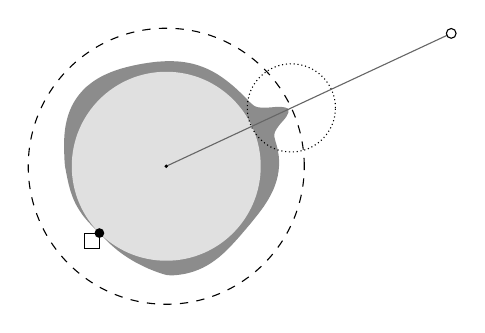
\begin{tikzpicture}[scale=0.8]
\fill[black!45] plot[smooth cycle,tension=0.6] coordinates {(1.790,0.000) (1.792,0.078) (1.787,0.156) (1.775,0.234) (1.759,0.310) (1.737,0.385) (1.718,0.460) (1.725,0.544) (1.795,0.653) (1.909,0.791) (1.941,0.905) (1.811,0.943) (1.612,0.931) (1.466,0.934) (1.383,0.968) (1.327,1.018) (1.276,1.070) (1.225,1.122) (1.173,1.173) (1.120,1.223) (1.066,1.271) (1.011,1.317) (0.954,1.362) (0.895,1.405) (0.835,1.446) (0.772,1.484) (0.708,1.519) (0.642,1.550) (0.574,1.578) (0.505,1.602) (0.435,1.623) (0.363,1.639) (0.291,1.652) (0.219,1.661) (0.146,1.666) (0.073,1.668) (0.000,1.668) (-0.073,1.664) (-0.145,1.659) (-0.217,1.651) (-0.289,1.641) (-0.361,1.630) (-0.433,1.617) (-0.505,1.603) (-0.577,1.586) (-0.650,1.568) (-0.722,1.548) (-0.794,1.525) (-0.865,1.499) (-0.936,1.469) (-1.006,1.437) (-1.074,1.400) (-1.140,1.359) (-1.203,1.313) (-1.264,1.264) (-1.320,1.209) (-1.372,1.151) (-1.419,1.089) (-1.462,1.023) (-1.499,0.955) (-1.530,0.884) (-1.557,0.810) (-1.578,0.736) (-1.595,0.660) (-1.607,0.585) (-1.615,0.509) (-1.620,0.434) (-1.622,0.360) (-1.622,0.286) (-1.620,0.213) (-1.617,0.141) (-1.614,0.070) (-1.607,0.000) (-1.594,-0.070) (-1.581,-0.138) (-1.567,-0.206) (-1.552,-0.274) (-1.535,-0.340) (-1.516,-0.406) (-1.493,-0.471) (-1.468,-0.534) (-1.439,-0.596) (-1.406,-0.656) (-1.370,-0.713) (-1.332,-0.769) (-1.291,-0.822) (-1.247,-0.873) (-1.202,-0.922) (-1.156,-0.970) (-1.108,-1.015) (-1.061,-1.061) (-1.015,-1.108) (-0.970,-1.156) (-0.923,-1.203) (-0.874,-1.249) (-0.824,-1.293) (-0.772,-1.336) (-0.717,-1.378) (-0.661,-1.418) (-0.603,-1.456) (-0.543,-1.493) (-0.482,-1.528) (-0.418,-1.561) (-0.353,-1.593) (-0.286,-1.624) (-0.218,-1.652) (-0.147,-1.679) (-0.074,-1.704) (-0.000,-1.726) (0.076,-1.733) (0.151,-1.729) (0.226,-1.720) (0.301,-1.707) (0.375,-1.689) (0.447,-1.667) (0.517,-1.640) (0.585,-1.609) (0.652,-1.573) (0.715,-1.534) (0.776,-1.491) (0.835,-1.446) (0.891,-1.398) (0.944,-1.349) (0.996,-1.298) (1.045,-1.246) (1.094,-1.193) (1.141,-1.141) (1.187,-1.088) (1.233,-1.034) (1.278,-0.981) (1.324,-0.927) (1.369,-0.872) (1.414,-0.816) (1.459,-0.760) (1.503,-0.701) (1.547,-0.641) (1.588,-0.578) (1.628,-0.513) (1.664,-0.446) (1.698,-0.376) (1.727,-0.304) (1.751,-0.231) (1.770,-0.155) (1.783,-0.078)};
\fill[black!12] (0,0) circle (1.500);
\draw[dashed] (0,0) circle (2.191);
\draw[densely dotted] (1.986,0.926) circle (0.700);
\draw[thin,black!60] (0,0) -- (4.524,2.109);
\filldraw[fill=white,draw=black] (-1.301,-1.301) rectangle (-1.061,-1.061);
\fill (-1.061,-1.061) circle (2.2pt);
\fill (0,0) circle (0.8pt);
\filldraw[fill=white,draw=black] (4.524,2.109) circle (2.2pt);
\end{tikzpicture}
\caption{The light disk is $B(0,b)$, the largest ball about the origin in~$D_n$, the dark region is $E=D_n\setminus B(0,b)$, and the dashed circle, of radius~$b+w$, contains~$D_n$. The square is a cell disjoint from~$D_n$ whose closure contains the point~$y_0$ (black dot) of the circle $\{|v|=b\}$, and every point of~$E$ contributes nonnegatively to~$U_E(y_0)$. The segment joins the origin (small dot) to $y_t=(b+w+4t)u$ (open dot) for a unit vector~$u$, and the points of~$E$ in the dotted ball $B((b+w)u,t)$ contribute negatively to~$U_E(y_t)$.}
\label{fig:contact}
\end{figure}

Fix $p>0$. In this section and the next we take $n$ large and work on the event of Section~\ref{sec:norm-event}; its complement has probability at most $Cn^{-p}$. With $K$ as in Section~\ref{sec:norm-event}, we have $D_n\subset B(0,Kr_n)$, and on this ball~\eqref{eq:approx} and $\max_x\ell_n(x)\leq Cr_n$ give, with~$\delta$ redefined for $d\geq3$,
\begin{equation}\label{eq:global}
|\widetilde\ell_n(y)-U_{D_n}(y)|\leq\delta,\qquad\text{where}\quad
\delta\coloneqq\begin{cases}C\sqrt{r_n}\log n,&d=2,\\C\sqrt{r_n\log n},&d\geq3\end{cases}\, .
\end{equation}

Let $b\coloneqq\Rin(n)$ and $E\coloneqq D_n\setminus B(0,b)$, as in Section~\ref{sec:largest-ball} for the Euclidean norm, and let $y_0$, $z$ and~$H$ be as there, so that
\begin{equation*}
|y_0|=b,\qquad\ell_n(z)=0,\qquad|z-y_0|\leq\sqrt d/2,\qquad|z|\geq b,\qquad H=U_{D_n}(y_0)=U_E(y_0)\, .
\end{equation*}

\subsection{The volume outside the inner ball}

If $s=|v|\geq b=|y_0|$, then
\begin{equation}\label{eq:contact-sign}
\frac{u_v\cdot(v-y_0)}{|v-y_0|^d}
=\frac{s^2-v\cdot y_0}{s|v-y_0|^d}
\geq\frac1{2s}|v-y_0|^{2-d}
\geq2^{1-d}s^{1-d}\, .
\end{equation}
The first inequality uses $2(s^2-v\cdot y_0)=|v-y_0|^2+s^2-b^2$, and the second $|v-y_0|\leq2s$ and $d\geq2$. Since $|v|\leq Cr_n$ on~$E$, integrating~\eqref{eq:contact-sign} over~$E$ gives $H\geq c|E|r_n^{1-d}$, and Lemma~\ref{lem:contact} gives
\begin{equation}\label{eq:mass}
|E|\leq Cr_n^{d-1}H\leq Cr_n^dq_n\, .
\end{equation}

\subsection{Upper bounds on the local times}

For a bounded measurable set~$D\subset\R^d$ and $y\in\R^d$, the potential of~$D$ with its negative contributions discarded is
\begin{equation*}
U_D^+(y)\coloneqq\frac{2\drift}{\omega_d}\int_D\left[u_v\cdot\frac{v-y}{|v-y|^d}\right]_+\dd v\, .
\end{equation*}
Suppose that $d\geq3$, let $\chi$ and~$A$ be as in Step~2 of the proof of Lemma~\ref{lem:contact}, and let $m$ be the function in~\eqref{eq:radial-convolution} for this~$\chi$. Since $0\leq m\leq\|\chi\|_1$, discarding the points~$v$ with $u_v\cdot(v-y)<0$ in~\eqref{eq:newton-convolution} with $D=E$ gives $\chi*U_E\leq\|\chi\|_1U_E^+$; also $|\chi*U_E|\leq\|\chi\|_1\sup|U_E|$. With~\eqref{eq:cone-convolution}, these two bounds give, for every $y\in\R^d$,
\begin{equation}\label{eq:potential-convolution}
(\chi*U_{D_n})(y)\leq\|\chi\|_1\bigl(U_{B(0,b)}(y)+\min\{U_E^+(y),\sup|U_E|\}\bigr)+C\log n\, .
\end{equation}
Since $U_E\leq\min\{U_E^+,\sup|U_E|\}$, the bounds~\eqref{eq:resolvent} with $\gamma=(2A)^{-1}$, \eqref{eq:convolution-bound} and~\eqref{eq:potential-convolution} give the first of the bounds
\begin{equation}\label{eq:envelopehigh}
\widetilde\ell_n(y)\leq C\bigl((b-|y|)_++\sup|U_E|+\log n\bigr)
\qquad\text{and}\qquad
\widetilde\ell_n(y)\leq C\bigl(U_E^+(y)+\log n\bigr)
\end{equation}
for every $y\in\R^d$, and the second for $|y|\geq b$, where $U_{B(0,b)}(y)=0$.

Suppose that $d=2$. By~\eqref{eq:global}, \eqref{eq:ballpotential-euclid}, \eqref{eq:potential-bound} and~\eqref{eq:mass}, every $y\in\R^2$ satisfies
\begin{equation}\label{eq:envelopeplanar}
\widetilde\ell_n(y)\leq2d\drift(b-|y|)_++Cr_n^{\nf34}(\log n)^{\nf14}\, ,
\end{equation}
since $\sqrt{r_n}\log n=o(r_n^{\nf34}(\log n)^{\nf14})$ and $\widetilde\ell_n$ vanishes outside~$B(0,Kr_n)$.

Let $L\coloneqq1+\max\{\ell_n(x):x\in\Z^d,\ |x|\geq b\}$. By~\eqref{eq:envelopehigh}, \eqref{eq:potential-bound} and~\eqref{eq:mass} when $d\geq3$, and by~\eqref{eq:envelopeplanar} when $d=2$,
\begin{equation}\label{eq:shellW}
L\leq Cr_nq_n^{\nf1d}\, .
\end{equation}

\subsection{The inner radius}

\begin{proof}[Proof of Proposition~\ref{prop:inner}]
By~\eqref{eq:radius-volume} and~\eqref{eq:mass},
\begin{equation*}
\left|1-\left(\frac b{r_n}\right)^{d+1}\right|
\leq C\bigl(r_n^{\nf{(1-d)}{2}}(\log n)^{\nf12}+r_n^{-1}+q_n\bigr)
\leq Cq_n\, ,
\end{equation*}
because $r_n^{\nf{(1-d)}{2}}(\log n)^{\nf12}\leq q_n$. This proves~\eqref{eq:inradius}. Since $D_n$ is the disjoint union of~$B(0,b)$ and~$E$, the bounds~\eqref{eq:inradius} and~\eqref{eq:mass} prove~(ii).

On~$B(0,Kr_n)$, the bounds~\eqref{eq:global}, \eqref{eq:ballpotential-euclid}, \eqref{eq:potential-bound} and~\eqref{eq:inradius} give
\begin{equation*}
\bigl|\widetilde\ell_n(y)-2d\drift(r_n-|y|)_+\bigr|
\leq C\bigl(\delta+r_nq_n+|E|^{\nf1d}\bigr)\leq Cr_nq_n^{\nf1d}\, ,
\end{equation*}
and outside~$B(0,Kr_n)$ both $\widetilde\ell_n(y)$ and $2d\drift(r_n-|y|)_+$ vanish, which proves~(iii).
\end{proof}

\section{The outer radius and the local times}\label{sec:outer}

We prove the bound on~$\Rout(n)$ in Theorem~\ref{thm:fluctuations}\,(i) (Proposition~\ref{prop:stronger-outer}) and the bound on the local times in Theorem~\ref{thm:fluctuations}\,(iii). We bound the largest local time outside the ball~$B(0,\Rin(n))$; the crossing estimate~\eqref{eq:euclid-crossing} then bounds $\Rout(n)-\Rin(n)$ by a constant times $\log n$ times one plus this local time. To bound this local time, we bound the volume of~$E=D_n\setminus B(0,\Rin(n))$ near the sphere of radius~$\Rout(n)+2\sqrt d$ about the origin. For a unit vector~$u$ and a number~$t$ with $\Rout(n)-\Rin(n)+2\sqrt d\leq t\leq\nf{r_n}{4}$, Step~1 of the proof of~\eqref{eq:outer-polylog} evaluates the potential at the point $y_t=(\Rout(n)+2\sqrt d+4t)u$ outside this sphere. The cell containing~$y_t$ is disjoint from~$D_n$, and its center is a site outside~$A_n$. Dynkin's formula at this center, with a bound on the bracket of the martingale, bounds~$U_{D_n}$ at this center, and~\eqref{eq:cellmodulus} transfers this bound to~$y_t$; the resulting bound on~$|U_E(y_t)|$ is~\eqref{eq:outer-probe-error}. The points of~$E$ in the ball of radius~$t$ about $(\Rout(n)+2\sqrt d)u$, the point of the sphere closest to~$y_t$, contribute negatively to~$U_E(y_t)$. Since $|U_E(y_t)|$ and the positive contributions to~$U_E(y_t)$ are small, the volume of~$E$ in this ball is small; the resulting bound on this volume is~\eqref{eq:outer-cap-mass}. Step~2 of the proof of~\eqref{eq:outer-planar} uses the same point~$y_t$ when $d=2$.

\begin{proposition}[Outer radius]\label{prop:stronger-outer}
Let $\gauge$ be the Euclidean norm, and let $0<\drift<\nf{1}{d}$. For every $p>0$ there exists $C(d,\drift,p)<\infty$ such that, for every integer~$n\geq2$, with probability at least $1-Cn^{-p}$,
\begin{equation*}
\Rout(n)\leq r_n+C\begin{cases}\sqrt{r_n}(\log n)^{\nf52},&d=2,\\(\log n)^{d+1},&d\geq3\end{cases}\, .
\end{equation*}
\end{proposition}

With $b=\Rin(n)$, $E=D_n\setminus B(0,b)$ and~$L$ as in Section~\ref{sec:contact}, let
\begin{equation*}
w\coloneqq\Rout(n)-b+2\sqrt d\, ,
\end{equation*}
so that $w\geq3\sqrt d/2\geq1$, because $b\leq\Rout(n)+\sqrt d/2$, and $E\subset\{b\leq|v|\leq b+w\}$. Then $b\asymp r_n$ and $b+w\asymp r_n$, by~\eqref{eq:inradius} and Proposition~\ref{prop:coarse}.

On the event of Section~\ref{sec:norm-event}, the bound~\eqref{eq:euclid-crossing} with $a=b=\Rin(n)$ gives $\Rout(n)\leq b+CL\log n$. Because $L\geq1$, this gives
\begin{equation}\label{eq:outer-width-occupation}
w\leq CL\log n\, ,
\end{equation}
and with~\eqref{eq:shellW} the first bound
\begin{equation}\label{eq:width-preliminary}
w\leq Cr_nq_n^{\nf1d}\log n=o\bigl(r_n(\log n)^{-d}\bigr)\, .
\end{equation}

\subsection{The potential beyond the inner radius}\label{sec:outer-potential}

Since $E$ lies in the annulus~$\{b\leq|v|\leq b+w\}$, Lemma~\ref{lem:layer} with $a=w$ gives
\begin{equation}\label{eq:annulus-potential}
\sup_{y\in\R^d}|U_E(y)|\leq2d\drift w\, .
\end{equation}

Both dimensions use the following deterministic bound on the positive contributions to the potential at a point between the two radii, in terms of the volume near the outer sphere.

\begin{lemma}\label{lem:near-far}
There exists $C(d,\drift)<\infty$ with the following property. Let $1\leq w\leq b$ and $\lambda\geq1$, and let $D$ be a measurable subset of $\{v\in\R^d:b\leq|v|\leq b+w\}$ such that $|D\cap B((b+w)u,t)|\leq\lambda t^{d-1}$ for every unit vector~$u$ and every $t\geq w$, and $\int_D|v-y|^{2-d}\dd v\leq\lambda b$ for every $y\in\R^d$. Then every $y\in\R^d$ with $b\leq|y|\leq b+w$ satisfies
\begin{equation*}
U_D^+(y)\leq C\bigl(\lambda w^{d-1}\bigr)^{\nf1d}+C\lambda\, .
\end{equation*}
\end{lemma}

\begin{proof}
Fix $y$ with $b\leq|y|\leq b+w$. If $t\geq w$, then $B(y,t)\subset B((b+w)u_y,2t)$, so $|D\cap B(y,t)|\leq2^{d-1}\lambda t^{d-1}$. In particular, the points of~$D$ within distance~$w$ of~$y$ have total volume at most $2^{d-1}\lambda w^{d-1}$, so, as in the proof of~\eqref{eq:potential-bound}, the integral of $|v-y|^{1-d}$ over them is at most $C(\lambda w^{d-1})^{\nf1d}$. For the other points~$v\in D$, both $|v|$ and~$|y|$ lie in~$[b,b+w]$, so the identity $2(|v|^2-v\cdot y)=|v-y|^2+|v|^2-|y|^2$ and $|v|^2-|y|^2\leq3bw$ give
\begin{equation*}
\left[u_v\cdot\frac{v-y}{|v-y|^d}\right]_+\leq\frac{2w}{|v-y|^d}+\frac1{2b|v-y|^{d-2}}\, .
\end{equation*}
The second term contributes at most $C\lambda$ to~$U_D^+(y)$, by the second hypothesis, and integrating the first by parts against the bound on $|D\cap B(y,t)|$ shows that it contributes at most $Cw\int_w^\infty\lambda t^{d-1}t^{-d-1}\dd t\leq C\lambda$.
\end{proof}

\subsection{The outer radius in higher dimensions}\label{sec:outer-high}

Suppose that $d\geq3$. Because the sphere of radius~$b+w$ is curved, the positive contributions of~$E$ to the potential at a point outside this sphere are at most a constant times
\begin{equation}\label{eq:curvature-size}
\Theta\coloneqq\log n+\frac1{r_n}\sup_{y\in\R^d}\int_E|v-y|^{2-d}\dd v\, .
\end{equation}
We prove that
\begin{equation}\label{eq:outer-polylog}
w\leq C(\log n)^{d+1}\, .
\end{equation}
By~\eqref{eq:outer-width-occupation} and~\eqref{eq:envelopehigh}, it suffices to bound $U_E^+(y)$ for $b\leq|y|\leq b+w$.

\begin{proof}[Proof of~\eqref{eq:outer-polylog}]
\emph{Step 1: The potential at a point of a cell disjoint from~$D_n$.} If $|y|\geq b+w$, then every $v\in E$ satisfies $|v|\leq|y|$, so the identity $2(|v|^2-v\cdot y)=|v-y|^2+|v|^2-|y|^2$ gives $u_v\cdot(v-y)\leq|v-y|^2/(2|v|)$; since $|v|\geq b\geq cr_n$ on~$E$, the definition~\eqref{eq:curvature-size} gives $U_E^+(y)\leq C\Theta$. Let $u$ be a unit vector, let $w\leq t\leq\nf{r_n}{4}$, let $y_t\coloneqq(b+w+4t)u$ (Figure~\ref{fig:contact}), and let $z\in\Z^d$ be the site with $y_t\in C_z$. Then $|z|\geq|y_t|-\sqrt d/2\geq b+w>\Rout(n)$, so $\ell_n(z)=0$, and the first sentence of Step~3 of the proof of Lemma~\ref{lem:contact}, with $x=y=z$, together with~\eqref{eq:convolution-bound}, \eqref{eq:potential-convolution} and $U_{B(0,b)}(z)=0$, gives $W_z\leq C(\chi*\widetilde\ell_n)(z)\leq C\Theta$, where $W_z$ is the sum in~\eqref{eq:bracket}. Hence~\eqref{eq:pointwise} and~\eqref{eq:localmart}, which apply at~$z$ because $|z|\leq Cr_n<3n$, together with~\eqref{eq:cellmodulus}, $U_{B(0,b)}(y_t)=0$ and $\Theta\geq\log n$, give
\begin{equation}\label{eq:outer-probe-error}
|U_E(y_t)|=|U_{D_n}(y_t)|\leq C\bigl(\sqrt{\Theta\log n}+\log n\bigr)\leq C\Theta\, .
\end{equation}

\emph{Step 2: The volume of~$E$ near the sphere of radius~$b+w$.} We show that, for every unit vector~$u$ and every $t\geq w$,
\begin{equation}\label{eq:outer-cap-mass}
|E\cap B((b+w)u,t)|\leq C\Theta t^{d-1}\, .
\end{equation}
For $t>\nf{r_n}{4}$ this follows from $|E|\leq Cr_n^{d-1}\log n$, which is~\eqref{eq:mass} for $d\geq3$, and $\Theta\geq\log n$, so let $w\leq t\leq\nf{r_n}{4}$, with $y_t$ as in Step~1. By Step~1, the positive parts of $u_v\cdot(v-y_t)|v-y_t|^{-d}$ contribute at most $C\Theta$ to~$U_E(y_t)$. If $v\in E\cap B((b+w)u,t)$, then $u_v\cdot u\geq(b+w-t)/(b+w)$, hence
\begin{equation*}
u_v\cdot(v-y_t)=|v|-(b+w+4t)u_v\cdot u
\leq(b+w)-(b+w+4t)\left(1-\frac t{b+w}\right)\leq-t\, ,
\end{equation*}
where the last inequality uses $t\leq\nf{r_n}{4}\leq(b+w)/2$, which holds for large~$n$ by~\eqref{eq:inradius}. Since also $|v-y_t|\leq5t$, we get $u_v\cdot(v-y_t)|v-y_t|^{-d}\leq-ct^{1-d}$ for each such~$v$. Thus $U_E(y_t)\leq C\Theta-ct^{1-d}|E\cap B((b+w)u,t)|$, which with~\eqref{eq:outer-probe-error} proves~\eqref{eq:outer-cap-mass}.

\emph{Step 3: The largest local time beyond the inner radius.} If $t\geq w$ and $b\leq|y|\leq b+w$, then $B(y,t)\subset B((b+w)u_y,2t)$, so~\eqref{eq:outer-cap-mass} gives
\begin{equation}\label{eq:outer-local-mass}
|E\cap B(y,t)|\leq C\Theta t^{d-1}\, .
\end{equation}
By~\eqref{eq:outer-cap-mass} and the definition~\eqref{eq:curvature-size} of~$\Theta$, Lemma~\ref{lem:near-far} applies to $D=E$ with $\lambda=C\Theta$ (here $w\leq b$ by~\eqref{eq:width-preliminary}), and gives $U_E^+(y)\leq C(\Theta w^{d-1})^{\nf1d}+C\Theta$ for $b\leq|y|\leq b+w$. Every site~$x\in A_n$ with $|x|\geq b$ satisfies $|x|\leq b+w$, so~\eqref{eq:envelopehigh} and $\Theta\geq\log n$ give
\begin{equation}\label{eq:outer-max-occupation}
L\leq C\bigl((\Theta w^{d-1})^{\nf1d}+\Theta\bigr)\, .
\end{equation}

\emph{Step 4: A bound on~$\Theta$.} Let $y\in\R^d$. If $t\geq w$ and $B(y,t)$ meets~$E$ at a point~$v_1$, then $B(y,t)\subset B(v_1,2t)$ and $|v_1|\in[b,b+w]$; so~\eqref{eq:outer-local-mass} and the bound $|E|\leq Cr_n^{d-1}\log n$ of~\eqref{eq:mass} give $|E\cap B(y,t)|\leq C\min\{\Theta t^{d-1},r_n^{d-1}\log n\}$ for $t\geq w$, while $|E\cap B(y,t)|\leq\omega_dt^d$ for $t<w$. Fubini's theorem and a split at $t=r_n(\log n/\Theta)^{\nf{1}{(d-1)}}$, where the two terms of the minimum agree, give
\begin{equation*}
\int_E|v-y|^{2-d}\dd v=(d-2)\int_0^\infty|E\cap B(y,t)|t^{1-d}\dd t\leq Cw^2+Cr_n\Theta^{\nf{(d-2)}{(d-1)}}(\log n)^{\nf{1}{(d-1)}}\, .
\end{equation*}
By~\eqref{eq:curvature-size} and Young's inequality, $\Theta\leq\nf\Theta2+C(w^2/r_n+\log n)$, so
\begin{equation}\label{eq:curvature-improved}
\Theta\leq C\bigl(w^2/r_n+\log n\bigr)\, .
\end{equation}

\emph{Step 5: The bound on~$w$.} By~\eqref{eq:outer-width-occupation}, \eqref{eq:outer-max-occupation} and Young's inequality,
\begin{equation*}
w\leq C\log n\bigl((\Theta w^{d-1})^{\nf1d}+\Theta\bigr)\leq\frac w2+C\Theta(\log n)^d\, ,
\end{equation*}
so $w\leq C\Theta(\log n)^d$, and~\eqref{eq:curvature-improved} gives
\begin{equation*}
w\leq C(\log n)^dw^2/r_n+C(\log n)^{d+1}\, .
\end{equation*}
By~\eqref{eq:width-preliminary}, $C(\log n)^dw/r_n\leq\nf12$ for large~$n$, so the first term on the right is at most~$\nf{w}{2}$, which proves~\eqref{eq:outer-polylog}.
\end{proof}

\subsection{The outer radius in the plane}\label{sec:outer-planar}

Suppose that $d=2$. We prove that
\begin{equation}\label{eq:outer-planar}
w\leq C\sqrt{r_n}(\log n)^{\nf52}\, .
\end{equation}
The argument follows Section~\ref{sec:outer-high} with $\sqrt{r_n\log n}$ in place of~$\Theta$, except that Step~1 bounds the sum~$W_x$ of~\eqref{eq:bracket} directly, since~\eqref{eq:envelopehigh} requires $d\geq3$.

\begin{proof}[Proof of~\eqref{eq:outer-planar}]
\emph{Step 1: Local times beyond the inner radius.} By~\eqref{eq:global}, \eqref{eq:ballpotential-euclid} and~\eqref{eq:annulus-potential}, every $x\in\Z^2$ satisfies
\begin{equation*}
\ell_n(x)\leq2d\drift(b-|x|)_++Cw+C\sqrt{r_n}\log n\, .
\end{equation*}
Let $x\in\Z^2$ satisfy $b\leq|x|\leq3n$. Since the local times vanish off~$A_n$, the sum~$W_x$ runs over $y\in A_n\subset B(0,Kr_n)$; bound each local time~$\ell_n(y)$ in it by this inequality: the terms~$2d\drift(b-|y|)_+$ contribute at most $Cr_n$ to~$W_x$, because $(b-|y|)_+\leq|y-x|$, and the other two terms at most $C(w+\sqrt{r_n}\log n)\log n=o(r_n)$, by~\eqref{eq:width-preliminary}. Hence $W_x\leq Cr_n$, so~\eqref{eq:localmart} gives $|\mathcal M_n^x|\leq C\sqrt{r_n\log n}$, and~\eqref{eq:pointwise} and $U_{B(0,b)}(x)=0$ give
\begin{equation}\label{eq:planar-exterior-pointwise}
|\ell_n(x)-U_E(x)|\leq C\sqrt{r_n\log n}\, .
\end{equation}

\emph{Step 2: Volume bounds and a bound on~$U_E^+$.} For $y_t=(b+w+4t)u$, where $u$ is a unit vector and $w\leq t\leq\nf{r_n}{4}$, the inequality $u_v\cdot(v-y_t)\leq|v-y_t|^2/(2|v|)$ of Step~1 of Section~\ref{sec:outer-high} bounds the positive contributions to~$U_E(y_t)$ by $C\int_E(2|v|)^{-1}\dd v\leq C|E|/r_n\leq C\sqrt{r_n\log n}$, by~\eqref{eq:mass}. At the site~$z$ with $y_t\in C_z$, the bound~\eqref{eq:planar-exterior-pointwise}, with $\ell_n(z)=0$ and~\eqref{eq:cellmodulus}, gives $|U_E(y_t)|\leq C\sqrt{r_n\log n}$. For each $v\in E\cap B((b+w)u,t)$, as in Step~2 of Section~\ref{sec:outer-high}, $u_v\cdot(v-y_t)|v-y_t|^{-2}\leq-ct^{-1}$, so, for every $t\geq w$,
\begin{equation*}
|E\cap B((b+w)u,t)|\leq Ct\sqrt{r_n\log n}\, ,
\end{equation*}
where the case $t>\nf{r_n}{4}$ follows from $|E|\leq Cr_n^{\nf32}(\log n)^{\nf12}$. Lemma~\ref{lem:near-far} applies to $D=E$ with $\lambda=C\sqrt{r_n\log n}$, because $|E|\leq Cr_n^{\nf32}(\log n)^{\nf12}\leq\lambda b$, and gives, for every $y$ with $b\leq|y|\leq b+w$,
\begin{equation}\label{eq:planar-positive-bound}
U_E^+(y)\leq C(r_n\log n)^{\nf14}\sqrt w+C\sqrt{r_n\log n}\, .
\end{equation}

\emph{Step 3: The bound on~$w$.} Since $U_E\leq U_E^+$, the bound~\eqref{eq:planar-exterior-pointwise} bounds $L$ by a constant times the right side of~\eqref{eq:planar-positive-bound}, and~\eqref{eq:outer-width-occupation} gives
\begin{equation*}
w\leq C\log n\Bigl((r_n\log n)^{\nf14}\sqrt w+\sqrt{r_n\log n}\Bigr)\leq\frac w2+C\sqrt{r_n}(\log n)^{\nf52}\, ,
\end{equation*}
which proves~\eqref{eq:outer-planar}.
\end{proof}

\begin{proof}[Proof of Proposition~\ref{prop:stronger-outer}]
On the event of Section~\ref{sec:norm-event}, for large~$n$, we have $\Rout(n)\leq b+w$ and, by~\eqref{eq:inradius}, $b-r_n\leq Cr_nq_n$, which is $C\log n$ when $d\geq3$ and $C\sqrt{r_n\log n}$ when $d=2$. So~\eqref{eq:outer-polylog} and~\eqref{eq:outer-planar} prove the proposition.
\end{proof}

\subsection{The uniform bound on the local times}\label{sec:global-profile}

We prove Theorem~\ref{thm:fluctuations}\,(iii) on the event of Section~\ref{sec:norm-event}. Suppose first that $d\geq3$. By~\eqref{eq:annulus-potential} and~\eqref{eq:outer-polylog}, $\sup|U_E|\leq Cw\leq C(\log n)^{d+1}$, which with~\eqref{eq:global}, \eqref{eq:ballpotential-euclid} and~\eqref{eq:inradius} gives
\begin{equation*}
\max_{y\in\Z^d,|y|\leq Kr_n}\bigl|\ell_n(y)-2d\drift(r_n-|y|)_+\bigr|
\leq C\bigl(\sqrt{r_n\log n}+(\log n)^{d+1}+|b-r_n|\bigr)
\leq C\sqrt{r_n\log n}
\end{equation*}
for large~$n$, since $|b-r_n|\leq C\log n$; outside~$B(0,Kr_n)$ both $\ell_n(y)$ and $2d\drift(r_n-|y|)_+$ vanish.

Let $d=2$. The function~$U_E$ is continuous (Section~\ref{sec:potential-bounds}), harmonic in~$B(0,b)$ because $E$ does not meet that ball and each coordinate of $(v-y)|v-y|^{-2}=-\nabla_y\log|v-y|$ is harmonic in $y\neq v$, and nonnegative on the closure of~$B(0,b)$ because $u_v\cdot(v-y)\geq0$ when $|v|\geq b\geq|y|$. The maximum principle, the inequality $U_E\leq U_E^+$, \eqref{eq:planar-positive-bound} and~\eqref{eq:outer-planar} give
\begin{equation*}
\sup_{|y|\leq b+w}U_E(y)\leq C\sqrt{r_n}(\log n)^{\nf32}\, .
\end{equation*}
For $|y|\leq b$, the bounds~\eqref{eq:global} and~\eqref{eq:ballpotential-euclid} give
\begin{equation*}
\bigl|\widetilde\ell_n(y)-2d\drift(r_n-|y|)_+\bigr|\leq C\bigl(\sqrt{r_n}(\log n)^{\nf32}+|b-r_n|\bigr)\, .
\end{equation*}
For $|y|\geq b$, the absolute value of this difference is at most the larger of $\widetilde\ell_n(y)$ and $2d\drift(r_n-|y|)_+$, which are nonnegative. Here $2d\drift(r_n-|y|)_+\leq2d\drift|b-r_n|$, and $\widetilde\ell_n(y)$ is at most $U_E(y)+C\sqrt{r_n}\log n$ by~\eqref{eq:global} if $|y|\leq b+w$ and vanishes otherwise. Since $|b-r_n|\leq C\sqrt{r_n\log n}$, restricting to sites proves Theorem~\ref{thm:fluctuations}\,(iii) for $d=2$.

\begin{proof}[Proof of Theorem~\ref{thm:fluctuations}]
On the event of Section~\ref{sec:norm-event}, for large~$n$, Proposition~\ref{prop:inner} gives the bounds on~$\Rin(n)$ and on the volume, Proposition~\ref{prop:stronger-outer} the bound on~$\Rout(n)$, and Section~\ref{sec:global-profile} the bound on the local times. The Borel--Cantelli lemma with $p>1$ gives the almost-sure statement.
\end{proof}

\section{Limit laws}\label{sec:sharp}

We prove central limit theorems and laws of the iterated logarithm for $\sum_{x\in A_n}|x|$ and for the local times at fixed sites. After centering, these quantities are, up to smaller errors, multiples of the quadratic martingale~$\mathcal Q$ of~\eqref{eq:quadratic} and of the martingales~$\mathcal M^y$ of Section~\ref{sec:dynkin}; we compute the limits of their brackets from Theorem~\ref{thm:shape}\,(ii), and then apply the martingale central limit theorem and the law of the iterated logarithm.

\subsection{The sum of the distances from the origin}

For the Euclidean norm, \eqref{eq:quadratic} reads
\begin{equation}\label{eq:moment-martingale}
\mathcal Q_n=2\drift\sum_{x\in A_n}|x|-n+|X_n|^2\, .
\end{equation}
Let $\Rmom(n)$ be the radius of the ball about the origin on which the integral of~$|v|$ equals $\sum_{x\in A_n}|x|$, that is,
\begin{equation}\label{eq:radial-moment-def}
\Rmom(n)\coloneqq\left(\frac{d+1}{d\omega_d}\sum_{x\in A_n}|x|\right)^{\nf{1}{(d+1)}}\, .
\end{equation}

\begin{theorem}[Sum of the distances from the origin]\label{thm:moment-fluctuations}
Let $\gauge$ be the Euclidean norm, let $0<\drift<\nf1d$, and let $\Rmom(n)$ be as in~\eqref{eq:radial-moment-def}. Then the following hold.
\begin{enumerate}[label=\textup{(\roman*)}]
\item \underline{\emph{Central limit theorem}}: as $n\to\infty$,
\begin{equation*}
\frac{\sum_{x\in A_n}|x|-n/(2\drift)}{r_n^{\nf{(d+3)}{2}}}
\xrightarrow{\mathrm d}\mathcal N\Bigl(0,\frac{2d\omega_d}{\drift(d+2)(d+3)}\Bigr)
\end{equation*}
and
\begin{equation*}
\frac{\Rmom(n)-r_n}{r_n^{\nf{(3-d)}{2}}}
\xrightarrow{\mathrm d}\mathcal N\Bigl(0,\frac{2}{\drift d\omega_d(d+2)(d+3)}\Bigr)\, .
\end{equation*}
\item \underline{\emph{Law of the iterated logarithm}}: for each choice of sign, almost surely,
\begin{align}
\limsup_{n\to\infty}\frac{\pm\bigl(\sum_{x\in A_n}|x|-n/(2\drift)\bigr)}{r_n^{\nf{(d+3)}{2}}\sqrt{2\log\log n}}
&=\Bigl(\frac{2d\omega_d}{\drift(d+2)(d+3)}\Bigr)^{\nf12}\, ,\notag\\
\limsup_{n\to\infty}\frac{\pm(\Rmom(n)-r_n)}{r_n^{\nf{(3-d)}{2}}\sqrt{2\log\log n}}
&=\Bigl(\frac{2}{\drift d\omega_d(d+2)(d+3)}\Bigr)^{\nf12}\, .\label{eq:moment-radius-lil}
\end{align}
\end{enumerate}
\end{theorem}

In the plane, comparing $\Rmom(n)$ with the inner and outer radii gives Theorem~\ref{thm:sharp}\,(ii) and, with a lower bound on the probability that~$\mathcal Q_n$ deviates by about $(\log n)^{\nf12}$ standard deviations (Lemma~\ref{lem:exp-deviation}), Theorem~\ref{thm:sharp}\,(i).

\begin{proof}[Proof of Theorem~\ref{thm:moment-fluctuations}]
\emph{Step 1: The bracket.} Under both~\eqref{eq:kernel} and the simple random walk transition probabilities, the conditional second-moment matrix of~$X_{j+1}-X_j$ given~$\mathcal F_j$ is $\nf1d$ times the identity, so for every $\mathcal F_j$-measurable random vector~$q$ the conditional variance of $q\cdot(X_{j+1}-X_j)$ is $|q|^2/d-\drift^2I_j(q\cdot u_{X_j})^2$. Since $\mathcal Q_{j+1}-\mathcal Q_j=2X_j\cdot(X_{j+1}-X_j+\drift I_ju_{X_j})$, the bracket of~$\mathcal Q$ is
\begin{equation}\label{eq:moment-exact-bracket}
\langle\mathcal Q\rangle_n=\frac4d\sum_{x\in\Z^d}\ell_n(x)|x|^2-4\drift^2\sum_{x\in A_n}|x|^2\, .
\end{equation}
By Theorem~\ref{thm:shape}\,(i), almost surely, for all large~$n$, $A_n\subset B(0,2r_n)$, and hence $\Rout(n)\leq2r_n+1$. With Theorem~\ref{thm:shape}\,(ii), this gives, almost surely,
\begin{equation*}
\frac1{r_n^{d+3}}\sum_{x\in\Z^d}\ell_n(x)|x|^2\longrightarrow
2d\drift\int_{|v|<1}(1-|v|)|v|^2\dd v=\frac{2d^2\drift\omega_d}{(d+2)(d+3)}\, .
\end{equation*}
The second sum in~\eqref{eq:moment-exact-bracket} is $O(r_n^{d+2})$, so
\begin{equation}\label{eq:moment-bracket-limit}
\frac{\langle\mathcal Q\rangle_n}{r_n^{d+3}}\longrightarrow\frac{8d\drift\omega_d}{(d+2)(d+3)}
\qquad\text{almost surely}\, .
\end{equation}

\emph{Step 2: The central limit theorem.} The increment bound $|\mathcal Q_{j+1}-\mathcal Q_j|\leq C|X_j|$ and $\Rout(n)=O(r_n)$ verify the conditional Lindeberg condition at scale~$r_n^{\nf{(d+3)}{2}}$. By~\eqref{eq:moment-bracket-limit} and~\citet[Corollary~3.1]{HallHeyde1980},
\begin{equation*}
\frac{\mathcal Q_n}{r_n^{\nf{(d+3)}{2}}}\xrightarrow{\mathrm d}\mathcal N\Bigl(0,\frac{8d\drift\omega_d}{(d+2)(d+3)}\Bigr)\, .
\end{equation*}

\emph{Step 3: The law of the iterated logarithm.} The predictable increment bound $C|X_{n-1}|$ satisfies Stout's condition: its ratio to $\sqrt{\langle\mathcal Q\rangle_n/\log\log\langle\mathcal Q\rangle_n}$ is $O(\sqrt{\log\log n/n})$. Thus~\citet{Stout1970} applies to both~$\mathcal Q$ and~$-\mathcal Q$, and~\eqref{eq:moment-bracket-limit} gives the required normalization.

\emph{Step 4: The sum and the radius.} In~\eqref{eq:moment-martingale}, $|X_n|^2=O(r_n^2)$ is negligible on both scales, giving the two limit laws for the sum. They imply $\Rmom(n)/r_n\to1$ almost surely. Expanding~\eqref{eq:radial-moment-def} at $n/(2\drift)$ gives
\begin{equation*}
\frac{\Rmom(n)-r_n}{r_n^{\nf{(3-d)}{2}}}
=\left(\frac1{d\omega_d}+o(1)\right)
\frac{\sum_{x\in A_n}|x|-n/(2\drift)}{r_n^{\nf{(d+3)}{2}}}\, .
\end{equation*}
Slutsky's lemma and the positive limiting factor give the assertions for~$\Rmom(n)$.
\end{proof}

\subsection{The potential at a fixed site}

Since $B(0,\Rin(n))\subset D_n\subset B(0,\Rout(n)+\sqrt d)$, Theorem~\ref{thm:fluctuations}\,(i) and~(ii) give, almost surely for all large~$n$, $|D_n\mathbin{\triangle}B(0,r_n)|\leq Cr_n^dq_n$ and, for every $v\in D_n\mathbin{\triangle}B(0,r_n)$,
\begin{equation}\label{eq:centering-shape-input}
\bigl||v|-r_n\bigr|\leq C\begin{cases}\sqrt{r_n}(\log n)^{\nf52},&d=2,\\(\log n)^{d+1},&d\geq3\end{cases}\, .
\end{equation}
The product of~$q_n$ and the right side of~\eqref{eq:centering-shape-input} is $C(\log n)^3$ when $d=2$ and $C(\log n)^{d+2}/r_n$ when $d\geq3$. On the annulus defined by~\eqref{eq:centering-shape-input}, the kernel~$|v|^{1-d}$ of~$U_{D_n}(0)$ is close to $r_n^{-d}|v|$, which relates $U_{D_n}(0)$ to $\sum_{x\in A_n}|x|$.

\begin{lemma}\label{lem:fixed-site-centering}
Let $\gauge$ be the Euclidean norm, let $0<\drift<\nf1d$, and let $y\in\Z^d$. There exists $C(d,\drift,y)<\infty$ such that, almost surely, for all sufficiently large~$n$,
\begin{equation}\label{eq:fixed-site-centering}
\left|U_{D_n}(y)-2d\drift(r_n-|y|)-\frac{\mathcal Q_n}{\omega_dr_n^d}\right|\leq C\begin{cases}(\log n)^3,&d=2,\\1,&d\geq3\end{cases}\, ,
\end{equation}
where $\mathcal Q$ is the martingale of~\eqref{eq:quadratic}.
\end{lemma}

By Theorem~\ref{thm:moment-fluctuations}, $\mathcal Q_n/(\omega_dr_n^d)$ has order~$r_n^{\nf{(3-d)}{2}}$, smaller than the order of~$\mathcal M^y_n$ by a factor~$(\log r_n)^{\nf12}$ in the plane and~$r_n^{\nf{(d-2)}{2}}$ when $d\geq3$.

\begin{proof}
Let $\nu\coloneqq\ind_{D_n}-\ind_{B(0,r_n)}$ and $U_\nu(y)\coloneqq(2\drift/\omega_d)\int\nu(v)u_v\cdot(v-y)|v-y|^{-d}\dd v$, so that $U_{D_n}=U_{B(0,r_n)}+U_\nu$ and $\|\nu\|_1\leq Cr_n^dq_n$. For large~$n$ the right side of~\eqref{eq:centering-shape-input} is at most~$\nf{r_n}{2}$, so $|v|\geq\nf{r_n}{2}$ wherever $\nu(v)\neq0$.

At the origin, the kernel is $u_v\cdot v|v|^{-d}=|v|^{1-d}$. The function $s\mapsto s^{1-d}-r_n^{-d}s$ vanishes at $s=r_n$ and has derivative $O(r_n^{-d})$ for $s\geq\nf{r_n}{2}$, so $\bigl||v|^{1-d}-r_n^{-d}|v|\bigr|\leq Cr_n^{-d}\bigl||v|-r_n\bigr|$ for $|v|\geq\nf{r_n}{2}$. Integrating against~$\nu$, with~\eqref{eq:centering-shape-input} and the bound on~$\|\nu\|_1$, and using $U_{B(0,r_n)}(0)=2d\drift r_n$ and $\int_{B(0,r_n)}|v|\dd v=n/(2\drift)$, gives
\begin{equation*}
\left|U_{D_n}(0)-2d\drift r_n-\frac{2\drift}{\omega_dr_n^d}\left(\int_{D_n}|v|\dd v-\frac{n}{2\drift}\right)\right|\leq C\begin{cases}(\log n)^3,&d=2,\\1,&d\geq3\end{cases}\, .
\end{equation*}
Replacing the integral by $\sum_{x\in A_n}|x|$ changes the expression in parentheses by $O(r_n^d)$, and~\eqref{eq:moment-martingale} proves~\eqref{eq:fixed-site-centering} at~$y=0$, since $|X_n|^2/(\omega_dr_n^d)=O(r_n^{2-d})=O(1)$.

For fixed~$y$, the gradient of $u_v\cdot(v-y)|v-y|^{-d}$ with respect to~$y$ is $O_y(r_n^{-d})$ for $|v|\geq\nf{r_n}{2}$, so $|U_\nu(y)-U_\nu(0)|=O_y(r_n^{-d}\|\nu\|_1)=O_y(1)$. With $U_{B(0,r_n)}(y)-U_{B(0,r_n)}(0)=-2d\drift|y|$, from~\eqref{eq:ballpotential-euclid}, this proves~\eqref{eq:fixed-site-centering}.
\end{proof}

\subsection{Local times at fixed sites}

Up to a smaller correction at first departures, the bracket of~$\mathcal M^y$ is a sum of local times with weights that decay like~$|x-y|^{2-2d}$; in the plane each dyadic annulus contributes the same order, which gives an extra factor~$\log r_n$. For functions $f_1,f_2\colon\Z^d\to\R$ with bounded nearest-neighbor increments, let
\begin{equation}\label{eq:site-gamma}
\Gamma(f_1,f_2)(x)\coloneqq\frac1{2d}\sum_{|e|=1}\bigl(f_1(x+e)-f_1(x)\bigr)\bigl(f_2(x+e)-f_2(x)\bigr)-\Delta f_1(x)\Delta f_2(x)\, ,
\end{equation}
which is the conditional covariance of the increments of~$\mathcal M^{f_1}$ and~$\mathcal M^{f_2}$ at a departure from~$x$ other than the first. As in Section~\ref{sec:dynkin}, $g_y=g(\cdot-y)$ and $G$ is the Green function.

\begin{theorem}[Local times at fixed sites]\label{thm:site-fluctuations}
Let $\gauge$ be the Euclidean norm, and let $0<\drift<\nf1d$. Then the following hold.
\begin{enumerate}[label=\textup{(\roman*)}]
\item \underline{\emph{Central limit theorem}}: for every $y\in\Z^d$, as $n\to\infty$,
\begin{equation}\label{eq:site-clt}
\begin{aligned}
\frac{\ell_n(y)-2d\drift(r_n-|y|)}{\sqrt{r_n\log r_n}}&\xrightarrow{\mathrm d}\mathcal N\Bigl(0,\frac{16\drift}{\pi}\Bigr)&&\text{if } d=2\, ,\\
\frac{\ell_n(y)-2d\drift(r_n-|y|)}{\sqrt{r_n}}&\xrightarrow{\mathrm d}\mathcal N\bigl(0,2d\drift(2G(0)-1)\bigr)&&\text{if } d\geq3\, .
\end{aligned}
\end{equation}
\item \underline{\emph{Law of the iterated logarithm}}: for every $y\in\Z^d$ and each choice of sign, almost surely,
\begin{equation*}
\begin{aligned}
\limsup_{n\to\infty}\frac{\pm(\ell_n(y)-2d\drift(r_n-|y|))}{\sqrt{2r_n\log r_n\log\log n}}&=\Bigl(\frac{16\drift}{\pi}\Bigr)^{\nf12}&&\text{if } d=2\, ,\\
\limsup_{n\to\infty}\frac{\pm(\ell_n(y)-2d\drift(r_n-|y|))}{\sqrt{2r_n\log\log n}}&=\bigl(2d\drift(2G(0)-1)\bigr)^{\nf12}&&\text{if } d\geq3\, .
\end{aligned}
\end{equation*}
\item \underline{\emph{Joint limits}}: for all $y_1,\ldots,y_k\in\Z^d$, the convergence in~\eqref{eq:site-clt} holds jointly for $y=y_1,\ldots,y_k$, and the limit is a centered Gaussian vector whose covariance matrix has $(i,j)$ entry
\begin{equation}\label{eq:site-covariance}
\begin{cases}
16\drift/\pi,&d=2,\\
2d\drift\bigl(2G(y_i-y_j)-\ind_{\{y_i=y_j\}}\bigr),&d\geq3
\end{cases}\, .
\end{equation}
\end{enumerate}
\end{theorem}

In the plane the limits at different sites are equal; this statement concerns finitely many fixed sites, whereas the maximum in Theorem~\ref{thm:sharp}\,(iii) is over the sites~$x$ with $|x|\leq r_n^{\nf12}$, a set that grows with~$n$.

\begin{proof}[Proof of Theorem~\ref{thm:site-fluctuations}]
\emph{Step 1: The bracket.} By~\eqref{eq:gradient}, at the first departure from~$x$ the conditional covariance of the increments of~$\mathcal M^y$ and~$\mathcal M^z$ differs from $\Gamma(g_y,g_z)(x)$ by $O_{y,z}((1+|x|)^{2-2d})$. By Theorem~\ref{thm:shape}\,(i), almost surely $A_n\subset B(0,Cr_n)$ for large~$n$, and summing over~$A_n$ gives, almost surely for large~$n$,
\begin{equation}\label{eq:site-bracket}
\langle\mathcal M^y,\mathcal M^z\rangle_n
=\sum_{x\in\Z^d}\ell_n(x)\Gamma(g_y,g_z)(x)
+\begin{cases}O_{y,z}(\log r_n),&d=2,\\O_{y,z}(1),&d\geq3\end{cases}\, .
\end{equation}

\emph{Step 2: The bracket in higher dimensions.} For $d\geq3$, the weights $\Gamma(g_y,g_z)$ are absolutely summable. Theorem~\ref{thm:shape}\,(ii), dominated convergence and summation by parts give, almost surely,
\begin{equation*}
\frac{\langle\mathcal M^y,\mathcal M^z\rangle_n}{r_n}
\longrightarrow2d\drift\sum_{x\in\Z^d}\Gamma(g_y,g_z)(x)
=2d\drift\bigl(2G(y-z)-\ind_{\{y=z\}}\bigr)\, .
\end{equation*}
The boundary term in the summation by parts is $O(r^{2-d})$ by~\eqref{eq:kernel-asymptotics} and~\eqref{eq:gradient}.

\emph{Step 3: The bracket in the plane.} Let $d=2$. By~\eqref{eq:kernel-asymptotics} and~\eqref{eq:gradient}, the increments of~$g_y$ at~$x$ are $(\nf{2}{\pi})e\cdot x/|x|^2+O_y(|x|^{-2})$, and $\sum_{|e|=1}(e\cdot x)^2=2|x|^2$. So, for fixed $y,z$ and as $|x|\to\infty$,
\begin{equation*}
\Gamma(g_y,g_z)(x)=\frac{2}{\pi^2|x|^2}+O_{y,z}(|x|^{-3})\, ,
\qquad\text{and hence}\qquad
\sum_{|x|\leq r}\Gamma(g_y,g_z)(x)=\frac4\pi\log r+O_{y,z}(1)\, .
\end{equation*}
In~\eqref{eq:site-bracket}, replacing $\ell_n(x)$ by $2d\drift(r_n-|x|)_+$ changes the sum by $o(r_n\log r_n)$, since the uniform error in Theorem~\ref{thm:shape}\,(ii) is $o(r_n)$ and $\sum_{|x|\leq Cr_n}|\Gamma(g_y,g_z)(x)|=O(\log r_n)$. For $|x|<r_n$ write $2d\drift(r_n-|x|)_+=2d\drift r_n-2d\drift|x|$: the constant term~$2d\drift r_n=4\drift r_n$ contributes $(16\drift/\pi)r_n\log r_n+O(r_n)$, and the term $-2d\drift|x|$ contributes $O(r_n)$, since $\sum_{|x|\leq Cr_n}|x|(1+|x|)^{-2}=O(r_n)$. Therefore
\begin{equation*}
\frac{\langle\mathcal M^y,\mathcal M^z\rangle_n}{r_n\log r_n}\longrightarrow\frac{16\drift}{\pi}
\qquad\text{almost surely}\, .
\end{equation*}

\emph{Step 4: Limit laws for the martingales.} The bounded increments and the bracket limits verify the hypotheses of the martingale central limit theorem~\citep[Corollary~3.1]{HallHeyde1980} and Stout's law~\citep{Stout1970}. The Cram\'er--Wold device gives the joint Gaussian limits for $(-\mathcal M_n^{y_i})_i$, including directions with zero limiting variance; Stout's law gives both signs of the almost-sure limits at each fixed site.

\emph{Step 5: The potential term.} By~\eqref{eq:pointwise},
\begin{equation*}
\ell_n(y)-2d\drift(r_n-|y|)=\bigl(U_{D_n}(y)-2d\drift(r_n-|y|)\bigr)-\mathcal M_n^y+O(\log n)\, .
\end{equation*}
Lemma~\ref{lem:fixed-site-centering} and Theorem~\ref{thm:moment-fluctuations} make the potential term and the error negligible on the normalizations for the central limit theorem and the law of the iterated logarithm. Step~4 therefore proves the theorem.
\end{proof}

\section{Lower bounds on the fluctuations}\label{sec:lower}

We prove the lower bounds of Theorem~\ref{thm:sharp}, an upper bound on the deviations of the local times away from the boundary (Proposition~\ref{prop:bulk-profile}), and logarithmic lower bounds on the radii (Proposition~\ref{prop:log-lower}). The lower bounds in Theorem~\ref{thm:sharp}\,(i), (iii) and~(iv)(a) need martingale deviations of about $(\log n)^{\nf12}$ standard deviations, which we obtain from exponential martingales (Lemma~\ref{lem:exp-deviation}): for parts~(i) and~(iv)(a) by the Paley--Zygmund inequality, and for part~(iii), where the deviation at a fixed site is typically smaller than the bound in part~(iii) by a factor of order~$(\log n)^{\nf12}$ (Theorem~\ref{thm:site-fluctuations}), by a second-moment bound for the average of the exponential martingales at many well-separated sites.

Throughout this section $0<\drift<\nf1d$, and $\Omega_n$ is the event of Section~\ref{sec:norm-event} with $p=10$, so $\P(\Omega_n^c)=O(n^{-10})$ and the estimates of Sections~\ref{sec:local}--\ref{sec:outer} used below hold on~$\Omega_n$ for large~$n$. In particular, by Section~\ref{sec:global-profile}, on~$\Omega_n$ for large~$n$,
\begin{equation}\label{eq:lower-local-error}
\max_{x\in\Z^d}\bigl|\ell_n(x)-2d\drift(r_n-|x|)_+\bigr|\leq Cr_n\lambda_n\, ,\qquad\text{where}\quad\lambda_n\coloneqq r_n^{-\nf12}(\log n)^{\nf32}\, .
\end{equation}

\begin{lemma}\label{lem:exp-deviation}
Let $0<c_0\leq C_0$. There exist $c(c_0,C_0)>0$ and $C(c_0,C_0)<\infty$ with the following property. Let $m$ and~$n$ be positive integers, let $b>0$, $\delta\geq0$ and $0\leq\alpha\leq1$, and let $S^1,\ldots,S^m$ be real martingales with respect to a common filtration, with $S^i_0=0$ and $|S^i_{t+1}-S^i_t|\leq b$ for $0\leq t<n$. Let $\Omega$ be an event with $\P(\Omega)\geq1-\alpha$ on which $c_0\leq\langle S^i\rangle_n\leq C_0$ for $1\leq i\leq m$. Then, for every real $\beta\geq C$ with $\beta b\leq c$, the following hold.
\begin{enumerate}[label=\textup{(\roman*)}]
\item For $1\leq i\leq m$,
\begin{equation*}
\P(S^i_n\geq c\beta)\geq\frac14e^{-C\beta^2}-\alpha
\qquad\text{and}\qquad
\P(S^i_n\leq-c\beta)\geq\frac14e^{-C\beta^2}-\alpha\, .
\end{equation*}
\item If $|\langle S^i,S^j\rangle_n|\leq\delta$ on~$\Omega$ for all $i\neq j$, and $\beta^2\delta+\beta^3b\leq1$, then
\begin{equation*}
\P\Bigl(\max_{1\leq i\leq m}S^i_n<c\beta\Bigr)\leq C\bigl(m^{-1}e^{C\beta^2}+\beta^2\delta+\beta^3b+e^{C\beta^2}\sqrt\alpha\bigr)\, .
\end{equation*}
\end{enumerate}
\end{lemma}

\begin{proof}
Let $(\mathcal G_t)_{0\leq t\leq n}$ be the filtration, let $\tau$ be the least integer $0\leq t<n$ such that $\langle S^i\rangle_{t+1}>2C_0$ for some~$i$, and let $\tau\coloneqq n$ if there is none. Since brackets are predictable, $\tau$ is a stopping time. The martingales~$S^i$ stopped at~$\tau$ have increments at most~$b$ and brackets at most~$2C_0$ at time~$n$, and on~$\Omega$ they agree with~$S^i$ up to time~$n$, because $\tau=n$ there. From now on $S^i$ denotes the stopped martingale; this changes neither the hypotheses nor~$S^i_n$ on~$\Omega$. Let $V_{ij}\coloneqq\langle S^i,S^j\rangle_n$, so that $|V_{ij}|\leq2C_0$ by the Cauchy--Schwarz inequality. We take $c\leq\min\{\nf14,\nf{c_0}8\}$ small and $C$ large, both depending only on $c_0$ and~$C_0$.

Let $Y$ be a random variable and $\mathcal H$ a $\sigma$-field with $\E(Y\mid\mathcal H)=0$ and $|Y|\leq b_1$, and let $s\in\R$ satisfy $|s|b_1\leq1$. Taylor's formula for the exponential and the logarithm gives, with an absolute implicit constant,
\begin{equation}\label{eq:exp-taylor}
\log\E\bigl(e^{sY}\bigm|\mathcal H\bigr)=\frac{s^2}2\E(Y^2\mid\mathcal H)+O\bigl(|s|^3b_1\E(Y^2\mid\mathcal H)\bigr)\, .
\end{equation}
Now let $S$ be a martingale with respect to~$(\mathcal G_t)$, with $S_0=0$, increments at most~$b_1$ and $\langle S\rangle_n\leq8C_0$, let $|s|b_1\leq\nf12$, and let
\begin{equation*}
K(s)\coloneqq\sum_{t<n}\log\E\bigl(e^{s(S_{t+1}-S_t)}\bigm|\mathcal G_t\bigr)
\qquad\text{and}\qquad
Z(s)\coloneqq\exp\{sS_n-K(s)\}\, .
\end{equation*}
By successive conditioning $\E Z(s)=1$, and~\eqref{eq:exp-taylor} gives $K(s)=s^2\langle S\rangle_n/2+O(|s|^3b_1)$. Hence $K(2s)-2K(s)\leq Cs^2$, and since $Z(s)^2=Z(2s)\exp\{K(2s)-2K(s)\}$, we get $\E Z(s)^2\leq e^{Cs^2}$. We apply the definitions and bounds of this paragraph with $s=\beta$ to~$S^i$, with $b_1=b$, and to $S^i+S^j$ for $i\neq j$, whose bracket at time~$n$ is $V_{ii}+V_{jj}+2V_{ij}\leq8C_0$, with $b_1=2b$; this is possible because $\beta b\leq\nf14$. Let $K_i$, $Z_i$ and $K_{ij}$, $Z_{ij}$ be the corresponding values of $K(\beta)$ and~$Z(\beta)$. Then
\begin{equation}\label{eq:exp-moments}
K_i=\frac{\beta^2}2V_{ii}+O(\beta^3b)
\qquad\text{and}\qquad
K_{ij}-K_i-K_j=\beta^2V_{ij}+O(\beta^3b)\, ,
\end{equation}
and $\E Z_i=\E Z_{ij}=1$, $\E Z_i^2\leq e^{C\beta^2}$ and $\E Z_{ij}^2\leq e^{C\beta^2}$.

We prove~(i). If $c$ is small enough, then on~$\Omega$ the bound $V_{ii}\geq c_0$ and~\eqref{eq:exp-moments} give $K_i\geq c_0\beta^2/4$. If also $C$ is large enough, then on~$\Omega$ the inequality $Z_i\geq\nf12$ implies $\beta S^i_n\geq c_0\beta^2/4-\log2$, hence $S^i_n\geq c_0\beta/8\geq c\beta$. By the Paley--Zygmund inequality, $\P(Z_i\geq\nf12)\geq(\E Z_i)^2/(4\E Z_i^2)\geq e^{-C\beta^2}/4$, so $\P(S^i_n\geq c\beta)\geq\P(\Omega\cap\{Z_i\geq\nf12\})\geq e^{-C\beta^2}/4-\alpha$. The same argument applied to~$-S^i$ gives the second bound in~(i).

We prove~(ii). Let $i\neq j$. By~\eqref{eq:exp-moments}, the exponent in $Z_iZ_j=Z_{ij}\exp\{K_{ij}-K_i-K_j\}$ is at most $\beta^2\delta+C\beta^3b$ on~$\Omega$, and at most $C\beta^2$ everywhere, because $|V_{ij}|\leq2C_0$ and $\beta b\leq1$. So the Cauchy--Schwarz inequality on~$\Omega^c$ and $\beta^2\delta+\beta^3b\leq1$ give
\begin{equation*}
\E(Z_iZ_j)\leq e^{\beta^2\delta+C\beta^3b}+e^{C\beta^2}\bigl(\E Z_{ij}^2\bigr)^{\nf12}\alpha^{\nf12}\leq1+C(\beta^2\delta+\beta^3b)+e^{C\beta^2}\sqrt\alpha\, .
\end{equation*}
Let $Z\coloneqq m^{-1}\sum_{i=1}^mZ_i$. Then $\E Z=1$, and the bounds on $\E Z_i^2$ and on $\E(Z_iZ_j)$ give
\begin{equation*}
\Var(Z)=\frac1{m^2}\sum_{i,j=1}^m\bigl(\E(Z_iZ_j)-1\bigr)\leq C\bigl(m^{-1}e^{C\beta^2}+\beta^2\delta+\beta^3b+e^{C\beta^2}\sqrt\alpha\bigr)\, .
\end{equation*}
On~$\Omega$, if $Z\geq\nf12$, then $Z_i\geq\nf12$ for some~$i$, and hence $\max_iS^i_n\geq c\beta$, as in the proof of~(i). So Chebyshev's inequality gives $\P(\max_iS^i_n<c\beta)\leq4\Var(Z)+\alpha$, which proves~(ii), because $\alpha\leq\sqrt\alpha$.
\end{proof}

\subsection{Lower bounds on the radii and their difference in the plane}

Up to additive constants, $\Rin(n)\leq\Rmom(n)\leq\Rout(n)$, and by~\eqref{eq:moment-martingale} the difference $\Rmom(n)-r_n$ is, to first order, proportional to~$\mathcal Q_n$. So Theorem~\ref{thm:sharp}\,(i) needs deviations of~$\mathcal Q_n$ of about $(\log n)^{\nf12}$ standard deviations with probability at least~$n^{-p}$. Lemma~\ref{lem:exp-deviation}\,(i) gives them, because on~$\Omega_n$ the bracket of~$\mathcal Q$ is close to the deterministic value $(4\pi\drift/5)r_n^5$. For part~(iv)(a) we apply Lemma~\ref{lem:exp-deviation}\,(i) to the first coordinate of the martingale~\eqref{eq:vector-def}, whose bracket lies between two constant multiples of~$n$ on the whole probability space, for part~(iv)(b) the martingale law of the iterated logarithm to the same coordinate, and for part~(iv)(c) the martingale central limit theorem to the martingale~\eqref{eq:vector-def} itself.

\begin{proof}[Proof of Theorem~\ref{thm:sharp}\,\textup{(i)} and~\textup{(ii)}]
\emph{Step 1: Comparison of the radii.} Comparison with unit cells gives, for every $r\geq1$,
\begin{equation*}
\sum_{x\in\Z^d,|x|<r}|x|=\frac{d\omega_d}{d+1}r^{d+1}+O(r^d)\, .
\end{equation*}
Every lattice site~$x$ with $|x|<\Rin(n)$ lies in~$D_n$, hence in~$A_n$, since the cells are disjoint and $x\in C_x$; also $A_n\subset B(0,\Rout(n)+1)$. So $\sum_{x\in A_n}|x|$ lies between the sums of~$|x|$ over the lattice sites in these two balls, and $s^{d+1}-t^{d+1}\geq(s-t)s^d$ for $s\geq t\geq0$ gives, for every path,
\begin{equation}\label{eq:moment-radius-comparison}
\Rin(n)\leq\Rmom(n)+C
\qquad\text{and}\qquad
\Rout(n)\geq\Rmom(n)-C\, .
\end{equation}

\emph{Step 2: The laws of the iterated logarithm.} By~\eqref{eq:moment-radius-comparison}, $r_n-\Rin(n)\geq r_n-\Rmom(n)-C$ and $\Rout(n)-r_n\geq\Rmom(n)-r_n-C$. For $d=2$ the right side of~\eqref{eq:moment-radius-lil} is $(20\pi\drift)^{-\nf12}$, so~\eqref{eq:moment-radius-lil} gives
\begin{equation*}
\limsup_{n\to\infty}\frac{r_n-\Rin(n)}{\sqrt{r_n\log\log n}}\geq\frac{\sqrt2}{\sqrt{20\pi\drift}}=\frac1{\sqrt{10\pi\drift}}\, ,
\end{equation*}
and the same bound for $\Rout(n)-r_n$, which proves~\eqref{eq:planar-lil-lower}.

\emph{Step 3: The polynomial lower bounds.} With $K$ as in Section~\ref{sec:norm-event}, $\Rout(n)<Kr_n$ on~$\Omega_n$. Let $\widehat{\mathcal Q}$ be~$\mathcal Q$ stopped when the walk first leaves~$B(0,Kr_n)$. Its increments are at most~$4Kr_n$, and on~$\Omega_n$ it agrees with~$\mathcal Q$ up to time~$n$, so $\langle\widehat{\mathcal Q}\rangle_n=\langle\mathcal Q\rangle_n$ on~$\Omega_n$, and~\eqref{eq:moment-exact-bracket} gives~$\langle\mathcal Q\rangle_n$. In the first sum of~\eqref{eq:moment-exact-bracket}, replacing $\ell_n(x)$ by $2d\drift(r_n-|x|)_+$ changes the sum by at most $Cr_n^5\lambda_n$, by~\eqref{eq:lower-local-error}, because $\ell_n$ and $2d\drift(r_n-|\cdot|)_+$ both vanish outside~$B(0,Kr_n)$; replacing the resulting lattice sum by the integral in Step~1 of the proof of Theorem~\ref{thm:moment-fluctuations} changes it by $O(r_n^4)$; and the second sum in~\eqref{eq:moment-exact-bracket} is $O(r_n^4)$. Since the limit in~\eqref{eq:moment-bracket-limit} is $4\pi\drift/5$ for $d=2$, this gives, on~$\Omega_n$ for large~$n$,
\begin{equation*}
\Bigl|\langle\widehat{\mathcal Q}\rangle_n-\frac{4\pi\drift}5r_n^5\Bigr|\leq Cr_n^5\lambda_n\leq\frac{2\pi\drift}5r_n^5\, .
\end{equation*}
Let $c_1>0$ and~$C_1$ be the constants of Lemma~\ref{lem:exp-deviation} for $c_0=2\pi\drift/5$ and $C_0=6\pi\drift/5$. Fix $p>0$, choose $a_p>0$ with $C_1a_p^2\leq\min\{p,10\}/2$, and let $\beta\coloneqq a_p(\log n)^{\nf12}$. For large~$n$, $\beta\geq C_1$ and $4K\beta r_n^{-\nf32}\leq c_1$. So Lemma~\ref{lem:exp-deviation}\,(i), with $m=1$, $S^1=\widehat{\mathcal Q}/r_n^{\nf52}$, $b=4Kr_n^{-\nf32}$, $\Omega=\Omega_n$ and $\alpha=\P(\Omega_n^c)=O(n^{-10})$, shows that each of the events $\{\mathcal Q_n\geq c_1\beta r_n^{\nf52}\}$ and $\{\mathcal Q_n\leq-c_1\beta r_n^{\nf52}\}$ has probability at least $n^{-\min\{p,10\}/2}/4-O(n^{-10})$ after intersection with~$\Omega_n$, since $\widehat{\mathcal Q}_n=\mathcal Q_n$ on~$\Omega_n$. On these intersections, by~\eqref{eq:moment-martingale} and $|X_n|^2\leq Cr_n^2$,
\begin{equation*}
\sum_{x\in A_n}|x|-\frac n{2\drift}\geq cr_n^{\nf52}(\log n)^{\nf12}
\qquad\text{and}\qquad
\frac n{2\drift}-\sum_{x\in A_n}|x|\geq cr_n^{\nf52}(\log n)^{\nf12}\, ,
\end{equation*}
respectively. Since $\Rmom(n)^3-r_n^3=(3/(2\pi))(\sum_{x\in A_n}|x|-n/(2\drift))$ and $\Rmom(n)\leq Cr_n$ on~$\Omega_n$, factoring the difference of cubes gives $\Rmom(n)-r_n\geq c\sqrt{r_n\log n}$ on the first intersection and $r_n-\Rmom(n)\geq c\sqrt{r_n\log n}$ on the second, so by~\eqref{eq:moment-radius-comparison} each event in~\eqref{eq:planar-polynomial-lower} has probability at least $n^{-\min\{p,10\}/2}/4-O(n^{-10})\geq n^{-p}$ for large~$n$.
\end{proof}

\begin{proof}[Proof of Theorem~\ref{thm:sharp}\,\textup{(iv)}]
Let $d=2$, let $V_n\coloneqq\sum_{x\in A_n}u_x$, and let $Z$ be the martingale~\eqref{eq:vector-def}, so that $Z_n=X_n+\drift V_n$, $Z_0=0$ and the increments of~$Z$ are at most~$2$. As in Step~1 of the proof of Theorem~\ref{thm:moment-fluctuations}, for every $q\in\R^2$ the increment of~$q\cdot Z$ at time~$j$ has conditional variance $|q|^2/2-\drift^2I_j(q\cdot u_{X_j})^2$, so
\begin{equation}\label{eq:width-bracket}
\langle q\cdot Z\rangle_n=\frac{|q|^2n}2-\drift^2\sum_{x\in A_n}(q\cdot u_x)^2\, .
\end{equation}
Let $Y_n\coloneqq e_1\cdot Z_n$, so that $Y_n=(X_n)_1+\drift(V_n)_1$ and $\nf{n}{2}-\drift^2|A_n|\leq\langle Y\rangle_n\leq\nf{n}{2}$.

\emph{Step 1: The sum over the range.} Every lattice site~$x$ with $|x|<\Rin(n)$ lies in~$A_n$, and the sum of~$u_x$ over these sites vanishes, by the symmetry $x\mapsto-x$. So $V_n$ is a sum of unit vectors over the sites~$x\in A_n$ with $\Rin(n)\leq|x|\leq\Rout(n)$, whose cells lie in the annulus $\{\Rin(n)-1\leq|v|\leq\Rout(n)+1\}$. Hence, for every path,
\begin{equation*}
|V_n|\leq C\bigl(\Rout(n)+1\bigr)\bigl(\Rout(n)-\Rin(n)+2\bigr)\, .
\end{equation*}
Suppose moreover that $\Rin(n)\geq\nf{r_n}{2}$ and $\Rout(n)\leq2r_n$, and let $e$ be a unit vector. Then $|u_x-u_v|\leq C/r_n$ for these sites~$x$ and $v\in C_x$, so comparison with the integral of $(e\cdot u_v)_+$ over the annulus, whose angular factor is $\int_0^{2\pi}(\cos\theta)_+\dd\theta=2$, gives $e\cdot V_n\leq\Rout(n)^2-\Rin(n)^2+Cr_n$; taking for~$e$ the direction of~$V_n$ gives
\begin{equation}\label{eq:width-annulus}
|V_n|\leq\Rout(n)^2-\Rin(n)^2+Cr_n\, .
\end{equation}

\emph{Step 2: The polynomial lower bound.} With $K$ as in Section~\ref{sec:norm-event}, $|(X_n)_1|\leq\Rout(n)<Kr_n$ on~$\Omega_n$. Since $\drift<\nf12$ and $|A_n|\leq n$, the martingale $S\coloneqq Y/\sqrt n$ has bracket at time~$n$ between $c_0\coloneqq\nf12-\drift^2>0$ and $C_0\coloneqq\nf12$ on the whole probability space, and increments at most $b\coloneqq2n^{-\nf12}$. Let $c_1>0$ and~$C_1$ be the constants of Lemma~\ref{lem:exp-deviation} for these $c_0$ and~$C_0$, fix $p>0$, choose $a_p>0$ with $C_1a_p^2\leq\min\{p,10\}/2$, and let $\beta\coloneqq a_p(\log n)^{\nf12}$. For large~$n$, $\beta\geq C_1$ and $\beta b\leq c_1$, so Lemma~\ref{lem:exp-deviation}\,(i), with $m=1$, the whole probability space in place of~$\Omega$ and $\alpha=0$, gives $\P(Y_n\geq c_1\beta\sqrt n)\geq n^{-\min\{p,10\}/2}/4$. On the intersection of this event with~$\Omega_n$, for large~$n$,
\begin{equation*}
\drift|V_n|\geq Y_n-|(X_n)_1|\geq c_1a_p\sqrt{n\log n}-Kr_n\geq\frac{c_1a_p}2\sqrt{n\log n}\, ,
\end{equation*}
and Step~1 gives $\Rout(n)-\Rin(n)\geq c\sqrt{n\log n}/r_n-2\geq c\sqrt{r_n\log n}$, because $n=(4\pi\drift/3)r_n^3$ by~\eqref{eq:radius}. Since $\P(\Omega_n^c)=O(n^{-10})$, this intersection has probability at least $n^{-\min\{p,10\}/2}/4-O(n^{-10})\geq n^{-p}$ for large~$n$, which proves~\eqref{eq:planar-width-polynomial}.

\emph{Step 3: The iterated logarithm.} By Theorem~\ref{thm:shape}, almost surely $|A_n|=O(r_n^2)=o(n)$ and $\Rin(n)+\Rout(n)\sim2r_n$. Hence $\langle Y\rangle_n/n\to\nf12$, and Stout's law for the martingale with bounded increments~$Y$ gives $\limsup Y_n/\sqrt{n\log\log n}=1$. Since $(X_n)_1=o(\sqrt n)$, the identity $Y_n=(X_n)_1+\drift(V_n)_1$ and~\eqref{eq:width-annulus} give
\begin{equation*}
\limsup_{n\to\infty}\frac{\Rout(n)-\Rin(n)}{\sqrt{r_n\log\log n}}
\geq\frac1{2\drift}\sqrt{\frac{4\pi\drift}{3}}
=\sqrt{\frac{\pi}{3\drift}}\, .
\end{equation*}

\emph{Step 4: Small differences of the radii.} Theorem~\ref{thm:shape} and~\eqref{eq:width-bracket} give $\langle q\cdot Z\rangle_n/n\to|q|^2/2$ for every~$q$. The bounded increments, the martingale central limit theorem and the Cram\'er--Wold device give $Z_n/\sqrt n\xrightarrow{\mathrm d}N$, where $N$ is a centered Gaussian vector with covariance matrix~$\nf12$ times the identity. Thus $\P(|N|\leq t)=1-e^{-t^2}$ for $t\geq0$.

By~\eqref{eq:width-annulus},
\begin{equation*}
|Z_n|\leq\drift\bigl(\Rout(n)-\Rin(n)\bigr)\bigl(\Rout(n)+\Rin(n)\bigr)+Cr_n\, .
\end{equation*}
Since $\Rout(n)+\Rin(n)\sim2r_n$ and $\sqrt n=(4\pi\drift/3)^{\nf12}r_n^{\nf32}$, the event $\{\Rout(n)-\Rin(n)\leq a\sqrt{r_n}\}$ forces $|Z_n|/\sqrt n\leq(3\drift/\pi)^{\nf12}a+o(1)$ almost surely. The portmanteau theorem and continuity of the radial Gaussian distribution give
\begin{equation*}
\limsup_{n\to\infty}\P\bigl(\Rout(n)-\Rin(n)\leq a\sqrt{r_n}\bigr)
\leq\P\bigl(|N|\leq(3\drift/\pi)^{\nf12}a\bigr)
=1-e^{-3\drift a^2/\pi}\, .
\end{equation*}
\end{proof}

\subsection{Upper bounds on the local times away from the boundary}

At sites~$y$ with $|y|\leq\theta r_n$, where $0<\theta<1$, the set $D_n\setminus B(0,\Rin(n))$ has small potential, because it has small volume and lies at distance of order~$r_n$ from~$y$; only the error~$\delta$ of~\eqref{eq:global} remains. In the plane the resulting bound improves Theorem~\ref{thm:fluctuations}\,(iii).

\begin{proposition}\label{prop:bulk-profile}
Let $\gauge$ be the Euclidean norm, let $0<\drift<\nf1d$, and let $0<\theta<1$ and $p>0$. There exists $C(d,\drift,\theta,p)<\infty$ such that, for every integer~$n\geq2$, with probability at least $1-Cn^{-p}$,
\begin{equation}\label{eq:bulk-profile}
\max_{\substack{y\in\Z^d\\|y|\leq\theta r_n}}\bigl|\ell_n(y)-2d\drift(r_n-|y|)\bigr|
\leq C\begin{cases}\sqrt{r_n}\log n,&d=2,\\\sqrt{r_n\log n},&d\geq3\end{cases}\, .
\end{equation}
The same bound holds for all sufficiently large~$n$ almost surely.
\end{proposition}

\begin{proof}
Intersect the events of Theorem~\ref{thm:fluctuations} and of Section~\ref{sec:norm-event}, with exponent $\max\{p,2\}$ in both, and let $E=D_n\setminus B(0,\Rin(n))$ as in Section~\ref{sec:contact}. For large~$n$, every~$y$ with $|y|\leq\theta r_n$ lies at distance at least $c_\theta r_n$ from~$E$, and Theorem~\ref{thm:fluctuations}\,(i) and~(ii) give $|E|\leq Cr_n^dq_n$; hence
\begin{equation*}
|U_E(y)|\leq C_\theta|E|r_n^{1-d}\leq C_\theta r_nq_n\, .
\end{equation*}
By Theorem~\ref{thm:fluctuations}\,(i), $|\Rin(n)-r_n|\leq Cr_nq_n$, so~\eqref{eq:ballpotential-euclid} gives, uniformly over $|y|\leq\theta r_n$,
\begin{equation}\label{eq:bulk-potential-only}
\bigl|U_{D_n}(y)-2d\drift(r_n-|y|)\bigr|\leq C_\theta r_nq_n\, .
\end{equation}
Since $r_nq_n\leq\delta$, with $\delta$ as in~\eqref{eq:global}, the bounds~\eqref{eq:global} and~\eqref{eq:bulk-potential-only} prove~\eqref{eq:bulk-profile} for large~$n$, and the Borel--Cantelli lemma gives the almost-sure statement.
\end{proof}

\subsection{Lower bounds on the local times near the origin}\label{sec:sharp-bulk}

By~\eqref{eq:pointwise} and~\eqref{eq:bulk-potential-only}, on~$\Omega_n$ the deviation $\ell_n(y)-2d\drift(r_n-|y|)$ at a site~$y$ with $|y|\leq\nf{r_n}{2}$ equals $-\mathcal M_n^y$ up to $O(r_nq_n+\log n)$. So it suffices to find, among about~$r_n^{\nf18}$ sites at mutual distances at least~$r_n^{\nf14}$, one at which $-\mathcal M_n^y$ exceeds a multiple of $(\log r_n)^{\nf12}$ standard deviations. In the plane the martingales at nearby sites are strongly correlated (see Step~3 of the proof of Theorem~\ref{thm:site-fluctuations}), so we use differences of martingales at two sites at distance about~$r_n^{\nf18}$. The normalized martingales then have brackets bounded above and below and cross brackets of order at most~$r_n^{-\nf14}$ (Lemma~\ref{lem:separated-brackets}), and Lemma~\ref{lem:exp-deviation}\,(ii) applies.

Recall the martingales~$\mathcal M^f$ of Section~\ref{sec:dynkin} and the function~$\Gamma(f_1,f_2)$ of~\eqref{eq:site-gamma}. Let $\sigma_n\coloneqq(r_n\log r_n)^{\nf12}$ and $k\coloneqq\lfloor r_n^{\nf18}\rfloor$ when $d=2$, and $\sigma_n\coloneqq r_n^{\nf12}$ when $d\geq3$. Let $m\coloneqq\lfloor r_n^{\nf18}\rfloor$, and for $1\leq i\leq m$ let
\begin{equation*}
y_i\coloneqq i\lceil r_n^{\nf14}\rceil e_1\, ,\qquad
f_i\coloneqq\begin{cases}g_{y_i+ke_1}-g_{y_i},&d=2,\\g_{y_i},&d\geq3\end{cases}
\qquad\text{and}\qquad
S^i\coloneqq-\frac{\mathcal M^{f_i}}{\sigma_n}\, .
\end{equation*}
Then $|y_i|\leq m\lceil r_n^{\nf14}\rceil\leq r_n^{\nf12}/2$ for large~$n$.

\begin{lemma}\label{lem:separated-brackets}
Let $\gauge$ be the Euclidean norm, and let $0<\drift<\nf1d$. There exist $0<c_0(d,\drift)\leq C_0(d,\drift)$ and $C(d,\drift)<\infty$ such that, for all sufficiently large~$n$, on~$\Omega_n$, for $1\leq i\leq m$ and $1\leq j\leq m$ with $j\neq i$,
\begin{equation*}
c_0\leq\langle S^i\rangle_n\leq C_0
\qquad\text{and}\qquad
|\langle S^i,S^j\rangle_n|\leq Cr_n^{-\nf14}\, .
\end{equation*}
\end{lemma}

\begin{proof}
\emph{Step 1: Sums of~$\Gamma(f_i,f_j)$.} For $d\geq3$, the second bound in~\eqref{eq:gradient} gives
\begin{equation*}
\sum_{x\in\Z^d}|\Gamma(f_i,f_j)(x)|\leq C
\quad\text{and}\quad
\sum_{x\in\Z^d}\min\{|x|,r_n\}|\Gamma(f_i,f_j)(x)|\leq C\bigl(r_n^{\nf12}+\log r_n\bigr)\, .
\end{equation*}
Bound the product of two increments by half the sum of their squares, and use $|x|\leq|x-y_i|+r_n^{\nf12}$. By~\eqref{eq:gradient}, $\max_{|e|=1}|f_i(x+e)-f_i(x)|^2\leq C(1+|x-y_i|)^{2-2d}$. The right side has bounded sum over all~$x$; its sum weighted by~$|x-y_i|$ over $|x-y_i|\leq r_n$ is $O(\log r_n)$ when $d=3$ and $O(1)$ when $d\geq4$; and its sum over $|x-y_i|>r_n$ is $O(r_n^{2-d})$.

For $d=2$, \eqref{eq:kernel-asymptotics} and~\eqref{eq:gradient} give
\begin{equation*}
\max_{|e|=1}|f_i(x+e)-f_i(x)|\leq\begin{cases}
C\bigl((1+|x-y_i|)^{-1}+(1+|x-y_i-ke_1|)^{-1}\bigr),&|x-y_i|\leq3k,\\
Ck(1+|x-y_i|)^{-2},&|x-y_i|>3k
\end{cases}\, .
\end{equation*}
The sum over~$x$ of the square of the right side is $O(\log r_n)$, and the same sum weighted by~$|x-y_i|$ is at most $Ck\log r_n$, so
\begin{equation*}
\sum_{x\in\Z^2}|\Gamma(f_i,f_j)(x)|\leq C\log r_n
\quad\text{and}\quad
\sum_{x\in\Z^2}\min\{|x|,r_n\}|\Gamma(f_i,f_j)(x)|\leq Cr_n^{\nf12}\log r_n\, .
\end{equation*}
The finitely supported products $\Delta f_i\cdot\Delta f_j$ satisfy the same bounds.

\emph{Step 2: The brackets.} Let
\begin{equation*}
\Sigma_{ij}\coloneqq\frac{2d\drift r_n}{\sigma_n^2}\sum_{x\in\Z^d}\Gamma(f_i,f_j)(x)\, .
\end{equation*}
We show that $|\langle S^i,S^j\rangle_n-\Sigma_{ij}|\leq C\lambda_n$ on~$\Omega_n$ for $1\leq i,j\leq m$; note that $\lambda_n\leq r_n^{-\nf14}$ for large~$n$. The bracket $\langle S^i,S^j\rangle_n$ equals $\langle\mathcal M^{f_i},\mathcal M^{f_j}\rangle_n/\sigma_n^2$. At a first departure from~$x$, the conditional covariance of the increments of~$\mathcal M^{f_i}$ and~$\mathcal M^{f_j}$ differs from $\Gamma(f_i,f_j)(x)$ by at most a constant times the product of the largest increments of $f_i$ and~$f_j$ at~$x$; on~$\Omega_n$ these differences sum over $x\in A_n$ to $O(1)$ when $d\geq3$ and $O(\log r_n)$ when $d=2$. In $\sum_x\ell_n(x)\Gamma(f_i,f_j)(x)$, replace $\ell_n(x)$ first by $2d\drift(r_n-|x|)_+$, which by~\eqref{eq:lower-local-error} changes the sum by at most $Cr_n\lambda_n\sum_x|\Gamma(f_i,f_j)(x)|$, and then by the constant~$2d\drift r_n$, which changes it by at most $2d\drift\sum_x\min\{|x|,r_n\}|\Gamma(f_i,f_j)(x)|$. With Step~1, this proves the bound $|\langle S^i,S^j\rangle_n-\Sigma_{ij}|\leq C\lambda_n$.

\emph{Step 3: The covariances.} For $d\geq3$, Step~2 of the proof of Theorem~\ref{thm:site-fluctuations} gives $\Sigma_{ij}=2d\drift(2G(y_i-y_j)-\ind_{\{i=j\}})$. So $\Sigma_{ii}=2d\drift(2G(0)-1)>0$, and for $i\neq j$ the absolute value of~$\Sigma_{ij}$ is $4d\drift G(y_i-y_j)=O(r_n^{\nf{(2-d)}{4}})$, by~\eqref{eq:kernel-asymptotics} and $|y_i-y_j|\geq r_n^{\nf14}$. For $d=2$, summation by parts on a ball of radius~$R$, followed by $R\to\infty$, gives
\begin{equation*}
\sum_{x\in\Z^2}\Gamma(f_i,f_j)(x)=2\bigl(g(y_i-y_j+ke_1)+g(y_i-y_j-ke_1)-2g(y_i-y_j)\bigr)-\sum_{x\in\Z^2}\Delta f_i(x)\Delta f_j(x)\, ,
\end{equation*}
where the last sum is $2$ if $i=j$ and $0$ otherwise, because the supports of $\Delta f_i$ and~$\Delta f_j$ are disjoint for $i\neq j$. So $\Sigma_{ii}=4\drift(4g(ke_1)-2)/\log r_n\to4\drift/\pi$ by~\eqref{eq:kernel-asymptotics}, and for $i\neq j$ the right side is $O(k^2/|y_i-y_j|^2)$ by~\eqref{eq:kernel-asymptotics}. Thus, in every dimension, the numbers~$\Sigma_{ii}$ lie between two positive constants for large~$n$, and for all $i\neq j$,
\begin{equation}\label{eq:bulk-correlation}
|\Sigma_{ij}|\leq Cr_n^{-\nf14}\, .
\end{equation}
With Step~2, this proves the lemma.
\end{proof}

\begin{proof}[Proof of Theorem~\ref{thm:sharp}\,\textup{(iii)}]
\emph{Step 1: The largest of the martingales.} By~\eqref{eq:gradient}, the increments of~$\mathcal M^{f_i}$ are bounded by a constant, so those of~$S^i$ are at most $b\coloneqq Cr_n^{-\nf12}$. Let $c_0$, $C_0$ and $\delta_n\coloneqq Cr_n^{-\nf14}$ be the bounds of Lemma~\ref{lem:separated-brackets}, and let $c_1>0$ and~$C_1$ be the constants of Lemma~\ref{lem:exp-deviation} for these $c_0$ and~$C_0$. Fix $a>0$ with $C_1a^2\leq\nf1{16}$, and let $\beta\coloneqq a(\log r_n)^{\nf12}$. For large~$n$, we have $\beta\geq C_1$, $\beta b\leq c_1$ and $\beta^2\delta_n+\beta^3b\leq1$. So Lemma~\ref{lem:exp-deviation}\,(ii), with $\delta=\delta_n$, $\Omega=\Omega_n$ and $\alpha=\P(\Omega_n^c)=O(n^{-10})$, and the bounds $m^{-1}\leq2r_n^{-\nf18}$, $e^{C_1\beta^2}\leq r_n^{\nf1{16}}$ and $r_n\leq n$ give
\begin{equation*}
\P\Bigl(\max_{1\leq i\leq m}S^i_n<c_1a(\log r_n)^{\nf12}\Bigr)
\leq C\bigl(r_n^{-\nf1{16}}+r_n^{-\nf14}\log r_n+r_n^{-\nf12}(\log r_n)^{\nf32}+r_n^{\nf1{16}-5}\bigr)
\leq Cr_n^{-\nf1{16}}\, .
\end{equation*}

\emph{Step 2: From the martingales to the local times.} On~$\Omega_n$ the bound~\eqref{eq:bulk-potential-only} with $\theta=\nf12$ holds for large~$n$. If $S^i_n\geq c_1a(\log r_n)^{\nf12}$ for some~$i$, then $-\mathcal M^{f_i}_n=\sigma_nS^i_n\geq c\sigma_n(\log r_n)^{\nf12}$, and $r_nq_n+\log n$ is of smaller order than $\sigma_n(\log r_n)^{\nf12}$. When $d\geq3$, the representation~\eqref{eq:pointwise} and~\eqref{eq:bulk-potential-only} give $\ell_n(y_i)-2d\drift(r_n-|y_i|)\geq-\mathcal M^{f_i}_n-C(r_nq_n+\log n)\geq c\sqrt{r_n\log n}$. When $d=2$, Dynkin's formula for~$f_i$ is the difference of~\eqref{eq:pointwise} at $y_i+ke_1$ and at~$y_i$, so~\eqref{eq:bulk-potential-only} gives
\begin{equation*}
\bigl|\bigl(\ell_n(y_i+ke_1)-2d\drift(r_n-|y_i+ke_1|)\bigr)-\bigl(\ell_n(y_i)-2d\drift(r_n-|y_i|)\bigr)\bigr|
\geq-\mathcal M^{f_i}_n-C(r_nq_n+\log n)\geq c\sqrt{r_n}\log n\, ,
\end{equation*}
and hence $|\ell_n(y)-2d\drift(r_n-|y|)|\geq\nf c2\sqrt{r_n}\log n$ at $y=y_i$ or at $y=y_i+ke_1$. All these sites satisfy $|y|\leq r_n^{\nf12}$. By Step~1, the probability that no index~$i$ has $S^i_n\geq c_1a(\log r_n)^{\nf12}$, plus $\P(\Omega_n^c)$, is at most $Cr_n^{-\nf1{16}}+Cn^{-10}$; since $r_n\asymp n^{\nf{1}{(d+1)}}$, this proves~\eqref{eq:sharp-bulk}.
\end{proof}

\subsection{Logarithmic lower bounds for the radii}

If $D_n$ contains~$B(0,r_n-h)$, or if $\Rout(n)\leq r_n+h$ and $d\geq3$, then the walk has visited many sites of an annulus of width of order~$h$ near the sphere of radius~$r_n$; in the second case this holds with high probability, by the martingale~$\mathcal Q$ of~\eqref{eq:moment-martingale}. From each such site the walk leaves $B(0,r_n+h)$ along a straight path with conditional probability at least~$e^{-Ch}$, so it follows none of these paths from $cr_n^{d-1}$ first arrivals on disjoint time intervals with probability at most $\exp\{-cr_n^{d-1}e^{-Ch}\}$.

\begin{proposition}[Lower bounds for the radii]\label{prop:log-lower}
Let $\gauge$ be the Euclidean norm, and let $0<\drift<\nf1d$. There exist $c(d,\drift)>0$, $C(d,\drift)<\infty$ and $h_0(d,\drift)>0$ such that the following hold.
\begin{enumerate}[label=\textup{(\roman*)}]
\item \underline{\emph{Tail bounds}}: for all sufficiently large~$n$ and every real~$h$ with $h_0\leq h\leq\nf{r_n}{8}$,
\begin{align}
\P\bigl(\Rin(n)\geq r_n-h\text{ and }\Rout(n)\leq r_n+h\bigr)&\leq\exp\bigl\{-cr_n^{d-1}e^{-Ch}\bigr\}\, ,\label{eq:log-lower-tail}\\
\P\bigl(\Rout(n)\leq r_n+h\bigr)&\leq\exp\bigl\{-cr_n^{d-1}e^{-Ch}\bigr\}+\exp\bigl\{-cr_n^{d-3}h^2\bigr\}\, .\label{eq:outer-lower-tail}
\end{align}
\item \underline{\emph{Almost-sure bounds}}: almost surely, for all sufficiently large~$n$,
\begin{equation}\label{eq:log-lower-as}
\max\{r_n-\Rin(n),\Rout(n)-r_n\}>c\log n\, ,
\end{equation}
and, if $d\geq3$, also $\Rout(n)-r_n>c\log n$.
\end{enumerate}
\end{proposition}

In the plane the last term in~\eqref{eq:outer-lower-tail} is not small when $h$ has order~$\log n$.

\begin{proof}
\emph{Step 1: Trials.} By~\eqref{eq:kernel}, every conditional nearest-neighbor transition probability is at least $p_0\coloneqq1/(2d)-\nf\drift2>0$. Let $T\coloneqq\lceil4h\sqrt d\rceil$. We show that, for every deterministic set $\Lambda\subset\{x\in\Z^d:|x|>r_n-2h\}$ and every integer $k>T$,
\begin{equation}\label{eq:lower-trials}
\P\bigl(\Rout(n)\leq r_n+h\text{ and }|A_n\cap\Lambda|\geq k\bigr)\leq(1-p_0^T)^j\, ,\qquad\text{where}\quad j\coloneqq\Bigl\lfloor\frac{k-T}{T+1}\Bigr\rfloor\, .
\end{equation}
From each $x\in\Lambda$, the path of $T$~steps in the direction $\operatorname{sgn}(x_i)e_i$, where $i$ is the smallest index with $|x_i|=\max_\ell|x_\ell|$, ends outside $B(0,r_n+h)$, because the derivative of $s\mapsto|x+s\operatorname{sgn}(x_i)e_i|$ on~$[0,\infty)$ is at least $|x_i|/|x|\geq d^{-\nf12}$. A trial starts at each first arrival at a site of~$\Lambda$ that occurs by time~$n-T$ and at or after the end of the preceding trial, and succeeds if the walk then follows this path from that site. If $|A_n\cap\Lambda|\geq k$, then at most $T$ of the first arrivals at sites of $A_n\cap\Lambda$ occur after time~$n-T$, and each trial interval contains at most $T+1$ of them, so at least $j$~trials start. Each trial starts at a stopping time, succeeds with conditional probability at least~$p_0^T$ given the history at that time, and ends no later than the next trial starts; so, by induction, the probability that at least $j$~trials start and the first $j$ fail is at most $(1-p_0^T)^j$. A successful trial ends outside $B(0,r_n+h)$ by time~$n$, which proves~\eqref{eq:lower-trials}.

\emph{Step 2: Two annuli.} Let $\mathcal S\coloneqq\{x\in\Z^d:r_n-2h<|x|<r_n-h-1\}$. After increasing~$h_0$, comparison with unit cells gives $|\mathcal S|\geq cr_n^{d-1}h$ for large~$n$. On $\{\Rin(n)\geq r_n-h\}$ every site of~$\mathcal S$ lies in~$D_n$, hence in~$A_n$. So~\eqref{eq:lower-trials} with $\Lambda=\mathcal S$ and $k=|\mathcal S|$, for which $k>T$ and $j\geq cr_n^{d-1}$ for large~$n$ because $T\leq Ch$, bounds the left side of~\eqref{eq:log-lower-tail} by $(1-p_0^T)^j\leq\exp\{-jp_0^T\}\leq\exp\{-cr_n^{d-1}e^{-Ch}\}$. In the same way, for $\Lambda\coloneqq\{x\in\Z^d:r_n-2h<|x|\leq r_n+h\}$ and every $c_1>0$,
\begin{equation}\label{eq:outer-lower-trials}
\P\bigl(\Rout(n)\leq r_n+h\text{ and }|A_n\cap\Lambda|\geq c_1r_n^{d-1}h\bigr)\leq\exp\{-cr_n^{d-1}e^{-Ch}\}\, ,
\end{equation}
where $c$ also depends on~$c_1$.

\emph{Step 3: Many sites of~$A_n$ in~$\Lambda$.} Let $I(s)\coloneqq\int_{B(0,s)}|v|\dd v$, so that $I(r_n)=n/(2\drift)$. By Jensen's inequality, $|x|\leq\int_{C_x}|v|\dd v$ for every site~$x$, so, after increasing $h_0$ so that $h_0\geq\sqrt d$, the sites with $|x|\leq r_n-2h$ contribute at most $I(r_n-2h+\sqrt d)\leq I(r_n-h)\leq I(r_n)-c_2r_n^dh$ to $\sum_{x\in A_n}|x|$, for a constant $c_2>0$. On $\{\Rout(n)\leq r_n+h\}$ every site of~$A_n$ satisfies $|x|\leq r_n+h\leq2r_n$, so $\sum_{x\in A_n}|x|\leq n/(2\drift)-c_2r_n^dh+2r_n|A_n\cap\Lambda|$. Let $c_1\coloneqq\nf{c_2}{4}$. If moreover $|A_n\cap\Lambda|<c_1r_n^{d-1}h$, then~\eqref{eq:moment-martingale} gives $\mathcal Q_n\leq-\drift c_2r_n^dh+(r_n+h)^2\leq-\drift c_2r_n^dh/2$ for large~$n$, after increasing~$h_0$ when $d=2$. The martingale~$\mathcal Q$ stopped at the first time~$\tau$ with $|X_\tau|>r_n+h$ starts at~$0$, has increments at most $4(r_n+h)\leq5r_n$, and equals~$\mathcal Q_n$ at time~$n$ on $\{\Rout(n)\leq r_n+h\}$, so Azuma's inequality and $n\leq Cr_n^{d+1}$ give
\begin{equation*}
\P\bigl(\Rout(n)\leq r_n+h\text{ and }|A_n\cap\Lambda|<c_1r_n^{d-1}h\bigr)
\leq\exp\Bigl\{-\frac{(\drift c_2r_n^dh)^2}{200nr_n^2}\Bigr\}\leq\exp\bigl\{-cr_n^{d-3}h^2\bigr\}\, .
\end{equation*}
With~\eqref{eq:outer-lower-trials}, this proves~\eqref{eq:outer-lower-tail}.

\emph{Step 4: The almost-sure bounds.} Take $h=c\log n$ with $c(d,\drift)>0$ small enough. The right side of~\eqref{eq:log-lower-tail} is summable, as is that of~\eqref{eq:outer-lower-tail} when $d\geq3$. The Borel--Cantelli lemma gives~(ii).
\end{proof}

\bibliographystyle{plainnat}
\bibliography{references}
\end{document}
